%/**
% * LaTeX thesis template (main file)
% * @author : Alexander willner <alex@willner.ws>
% * @url    : http://github.com/thesis
% */

% include config ---------------------------------------------------------------
\RequirePackage{pdf14}                 % PDF/A2-b compatibility
%\PassOptionsToPackage{demo}{graphicx} % for faster drafts
% document configuration -------------------------------------------------------
\documentclass[
        %pagesize,              % put paper size information into document
        a4paper,                % use a5paper for ISO A5; use a4paper for ISO A4
        pdftex,                 % PDF output
        %fontsize=12pt,         % font size
        headsepline,            % use headinclude also! (see M. Kohm)
        footsepline,            % use footinclude also! (see M. Kohm)
        %headinclude,            % count head to text body (not to margin)
        %footinclude,            % count foot to text body (not to margin)
        %BCOR8mm,               % set extra margin for book fixation
        headsepline,            % line on the top
        titlepage,              % show a title page
        %draft,                 % show under-/overfull boxes, hide images
        %demo=true,             % faster compile time
        %DIV=calc,              % calculate a nice type area
        %listof=totoc,          % List of Listings to ToC
        %oneside,               % e.g. same headings for odd and even pages
        %oneside=true,          % e.g. same headings for odd and even pages
        %twoside=false,         % e.g. same headings for odd and even pages
        %open=any,              % allows chapters to occur on left hand pages
        %openany,               % allows chapters to occur on left hand pages
        %ngerman,               % German language support
        %numbers=noendperiod    % no number at the end (German DUDEN)
%]{scrbook}
]{book}
% ------------------------------------------------------------------------------


% lang config ------------------------------------------------------------------
\usepackage[english]{babel}                  % English language support
%\usepackage[ngerman,english]{babel}         % German language support
%\usepackage{bibgerm}                        % German bibliography support
%\usepackage[babel,german=quotes]{csquotes}  % German language support
% ------------------------------------------------------------------------------


% basic packages ---------------------------------------------------------------
%\usepackage{tocloft}                         % Tweaks for large ToCs
%\cftsetpnumwidth{2em}                        % Tweaks for large ToCs
%\usepackage[demo]{graphicx}                  % faster compile time
\input{lib/resources/config/default}          % Default config
\usepackage[babel]{csquotes}                  % Biber wants it for babel
\usepackage[export]{adjustbox}                % For boxes around images
\usepackage{needspace}                        % used for embedding listings
%\usepackage{idxlayout}                       % fix index bugs and allow config
% ------------------------------------------------------------------------------

% basic config -----------------------------------------------------------------
\definecolor{LinkColor}{rgb}{0.0,0.2,0.5}     % Link color
\definecolor{MarginColor}{rgb}{0.0,0.2,0.5}   % Margin color
\definecolor{CaptionColor}{rgb}{0.0,0.2,0.5}  % Caption color
\definecolor{disabled}{gray}{0.5}             % Disabled text color
%\addtokomafont{sectioning}{\rmfamily}         % Serifs in headings
%\addtokomafont{sectioning}{\normalfont\scshape\rmfamily\color{CaptionColor}} % Serifs in headings
%\addtokomafont{sectioning}{\normalfont\rmfamily\color{CaptionColor}}        % Serifs in headings
\renewcommand{\lstlistlistingname}{List of Listings}
\renewcommand{\lstlistingname}{Listing}
\renewcommand{\contentsname}{Table of Contents}
\setcounter{secnumdepth}{4}
\setcounter{tocdepth}{2}
% basic config -----------------------------------------------------------------


% local config -----------------------------------------------------------------
\usepackage{pdflscape}
%\usepackage{subfig}
\usepackage{xmpincl}
%\includexmp{an-xmp-file-if-you-like}
\usepackage{enumitem}                   % More compact listings
\usepackage{float}                      % Provides the H float modifier option
% ------------------------------------------------------------------------------


% bibliography -----------------------------------------------------------------
\usepackage[
            style=numeric,%ieee,
            sorting=none,
            backref,
            backend=biber,
            defernumbers=true,
            useprefix=true,
            giveninits=true,
            %maxcitenames=2,
            maxbibnames=99, minbibnames=99,
            %doi=false,isbn=false,url=false,
            ]{biblatex}
\addbibresource{thesis_template.bib}
\defbibheading{empty}{}
\DeclareBibliographyCategory{cited}
\AtEveryCitekey{\addtocategory{cited}{\thefield{entrykey}}}
% ------------------------------------------------------------------------------


% acronyms ---------------------------------------------------------------------
\usepackage{acro}
\acsetup{
            single=false,
            list/sort=true,
            list/template=longtable,
            index/use, %  migh result in 'pdfTeX warning (dest): name... has been referenced but does not exist, replaced by a fixed one'
            pages/display=first,
}
\robustify\footnote%
\robustify\url%

\makeatletter\newif\ifnewacro%
\@ifpackagelater{acro}{2015/08/15}{% version 2.0 or later
\setboolean{newacro}{true}
}{% else hide footnotes and citations
\setboolean{newacro}{false}
\typeout{warning: your acro package is too old (<2.0)}
}%
\makeatother
% ------------------------------------------------------------------------------


% more config ------------------------------------------------------------------
% todo: move to 'basic config'
\usepackage{lmodern}                          % Nicer fonts (for all) - times
\usepackage{mathptmx}                         % Nicer fonts (for all) - times
%\usepackage{scrhack}                         % Fix some scrbook issues
\usepackage{scrlayer-scrpage}                 % before titlesec 
\usepackage{chapterthumb}                     % Fancy thumb index
\usepackage[chapter]{algorithm}               % Nice pseudo code
\usepackage{lettrine}                         % Drop characters, if you like
\renewcommand{\LettrineFontHook}{\color{CaptionColor}}
\usepackage[nohints]{minitoc}                 % ToC for chapters
\dominitoc[n]                                 % ToC: no caption
\renewcommand{\mtcSfont}{\small}              % ToC: small
\usepackage{makeidx}                          % Make an index
\makeindex                                    % Make an index
% ------------------------------------------------------------------------------

% chapter layout ---------------------------------------------------------------
%\usepackage[Sonny]{fncychap}                  % Nice chapter header
%\ChNameVar{\vspace*{-1in}\Large\rmfamily\vspace*{-2in}}   % Fancy chapter with serifs
%\ChTitleVar{\color{CaptionColor}\Large\rmfamily\scshape}  % Fancy chapter with serifs
\usepackage[clearempty]{titlesec}            % Suppress header and footer for empty pages
\setlength{\headheight}{1.1\baselineskip}
\titleformat{\chapter}[display]
  {\scshape\huge\color{CaptionColor}}
  {\filleft\Large\chaptertitlename~\thechapter}
  {2.5ex}
  {\titlerule\vspace{1ex}\filleft}
  [\vspace{1ex}\titlerule]
% ------------------------------------------------------------------------------

% spqueezing -------------------------------------------------------------------
%\usepackage{etoolbox}
%\makeatletter
%\patchcmd{\AC@@acro}
%  {\dotfill\pageref{acro:#1}}
%  {\nobreak\leaders\hbox{$\mkern -7mu \mkern \@dotsep mu\hbox{.}\mkern \@dotsep mu \mkern 7mu$}%
%   \hfill\nobreak\makebox[1.3em][r]{\pageref{acro:#1}}}
%  {}
%  {}
%\makeatother
% ------------------------------------------------------------------------------


% wall papger / logo on first page ---------------------------------------------
 \usepackage{wallpaper}
 \newlength\cornerXoffset%
 \newlength\cornerYoffset%
 \setlength\cornerXoffset{2cm}        % X
 \setlength\cornerYoffset{2cm}        % Y
 \newcommand\ThisLROffsetCornerWallPaper[2]{%
  \AddToShipoutPicture*{%
    \AtPageLowerLeft{%
      \parbox[b]{\paperwidth-\cornerXoffset}{%
        \hfill \includegraphics[width=#1\paperwidth,height=#1\paperheight,%
        keepaspectratio]{#2}%
        \vspace{\cornerYoffset}\null%
      }
    }
  }
 }
% ------------------------------------------------------------------------------


% page layout ------------------------------------------------------------------
%  \usepackage[ % Optional page bleed
%    cross, # some printing services might not like it others may require it...
%    center,
%    width=216mm, % A4 + 6mm
%    height=303mm % A4 + 6mm
%  ]{crop}
\usepackage[pass,a4paper]{geometry}
%\usepackage[marginparwidth=.7in, marginparsep=0.2in]{geometry}
%\geometry{a4paper, bottom=4cm}
% \renewcommand{\topfraction}{0.9}
% \renewcommand{\bottomfraction}{0.9}
% \renewcommand{\textfraction}{0.07}         % allow minimal text w. figs
% \renewcommand{\floatpagefraction}{0.7}     % require fuller float pages
% \renewcommand{\dblfloatpagefraction}{0.7}  % require fuller float pages
% \renewcommand{\dbltopfraction}{0.9}        % fit big float above 2-col. text
% \renewcommand{\textfloatsep}{5mm}
% \setcounter{topnumber}{2}
% \setcounter{bottomnumber}{2}
% \setcounter{totalnumber}{4}                % 2 may work better
% \setcounter{dbltopnumber}{2}               % for 2-column pages
% ------------------------------------------------------------------------------


% hyperlinks (almost last package) ---------------------------------------------
\usepackage{hyperxmp}                 % Semantic meta data (RDF/XMP)
%\pdfminorversion=4                   % PDF/A compatbility
%\pdfobjcompresslevel=0               % PDF/A compatbility
%\pdfcompresslevel=0                  % PDF/A compatbility
\usepackage[pdftex,                   % Hyperlinks in PDFs
pdfa=true,                            % PDF/A compatbility (fix hyperlink with ghostscript)
pdfapart=1,                           % PDF/A compatbility
unicode=true,                         % PDF/A compatbility
raiselinks=true,			                % calculate real height of the link
breaklinks,                           % break links
%backref=page,                        % backlinks in bibliography (section, slide, page, none)
%pagebackref=true,                    % backlinks in bibliography
hyperindex=true,                      % backlinkex index
linktocpage=true,                     % ToC links pages
bookmarks=true,                       % Bookmarks for PDF viewers
bookmarksopen=true,                   % Open bookmarks
bookmarksopenlevel=2,                 % How many levels to open
bookmarksnumbered=true,               % Numbers in the bookmarks
bookmarkstype=toc,                    % Type of bookmark
plainpages=false,                     % Anchors even on plain pages?
pageanchor=true,                      % Pages are linkable
pdfstartview=FitH,                    % Open document with Fit Width
pdfpagelabels=true,                   % set PDF page labels
pdfpagemode=UseOutlines,              % Show bookmarks in viewer
colorlinks,                           % Show colored links
linkcolor=LinkColor,                  % Link color
urlcolor=LinkColor,                   % URL color
anchorcolor=LinkColor,                % Anchor color
citecolor=LinkColor,                  % Cite color
menucolor=LinkColor,                  % Menu color
hypertexnames=true                    % Whatever ;)
]{hyperref}                           % Use hyperlinks
%\renewcommand*{\backref}[1]{[cited at page #1]} % Show formatted backlinks
\usepackage{bookmark}                 % Manually add PDF bookmarks
\hypersetup{keeppdfinfo}              % fix for hyperxmp, however, breaks PDF/A compliance
% ------------------------------------------------------------------------------


% cleveref with fixes ----------------------------------------------------------
\usepackage{cleveref}                 % To ref footnotes twice (use after hyperref)
\crefformat{footnote}{#2\footnotemark[#1]#3}
% ------------------------------------------------------------------------------


% glossary (last package) ----------------------------------------------------
\usepackage[xindy,nonumberlist,toc]{glossaries}
\input{thesis_template.glos.tex}
\setglossarystyle{altlist}
\renewcommand*{\glsgroupskip}{}
\makeglossaries%
% ------------------------------------------------------------------------------


% meta data --------------------------------------------------------------------
% meta data --------------------------------------------------------------------
\newcommand{\metaType}{PhD of templates}
\newcommand{\metaTypeShort}{Dr.-Tmpl.}
\newcommand{\metaWhy}{To get the degree in}
\newcommand{\metaHowFinal}{Submitted}
\newcommand{\metaHowNonFinal}{Draft}
\newcommand{\metaBoard}{Board}
\newcommand{\metaSubmitted}{Presented by}
\newcommand{\metaDate}{30.09.2021}
\newcommand{\metaDateEn}{16.~June~2020}
\newcommand{\metaDateExam}{\metaDate}
\newcommand{\metaNumber}{2020--06}
\newcommand{\metaTitleLayouted}{Sophisticated Template\\for a Thesis}
\newcommand{\metaTitle}{Exploration of methods for in-hand slip detection with an event-based camera during pick-and-place motions}
\newcommand{\metaTitleShort}{Thesis Template}
\newcommand{\metaDegree}{MTA}
\newcommand{\metaBirthplace}{Born in Foo Bar}
\newcommand{\metaAuthor}{First Last}
\newcommand{\metaAuthorMail}{first.last@example.org}
\newcommand{\metaKeywords}{Foo, Bar, First, Last}
\newcommand{\metaSubject}{Template Subject}
\newcommand{\metaUniversity}{Template University}
\newcommand{\metaFaculty}{Template Faculty}
\newcommand{\metaDepartment}{Template Department}
\newcommand{\metaCitycode}{12345}
\newcommand{\metaCity}{Berlin}
\newcommand{\metaCountry}{Country}
\newcommand{\metaURL}{http://example.org}
\newcommand{\metaChair}{Chair}
\newcommand{\metaChairName}{Prof.\ Dr.-Ing.\ Goo Gl}
\newcommand{\metaChairUniversity}{Industry}
\newcommand{\metaReviewer}{Reviewer}
\newcommand{\metaFirstReviewerName}{Prof.\ Dr.-Ing.\ Foo Bar}
\newcommand{\metaFirstReviewerUniversity}{Example University}
\newcommand{\metaSecondReviewerName}{Prof.\ Dr.\ Bar Foo}
\newcommand{\metaSecondReviewerUniversity}{Another University}
\newcommand{\metaThirdReviewerName}{Dr.\ John Smith}
\newcommand{\metaThirdReviewerUniversity}{My University}
\newcommand{\metaFourthReviewerName}{{\color{gray}Dr.\ Jon Doe}}
\newcommand{\metaFourthReviewerUniversity}{{\color{gray}BAR}}


\newcommand{\metaAuthorShort}{\metaAuthor}
\newcommand{\metaConference}{Conference}
\newcommand{\metaConferenceArea}{Area}
\newcommand{\metaDedication}{\scriptsize{Dedicated to my beloved family.}}
% ------------------------------------------------------------------------------

\input{lib/resources/config/pdfmetadata}
% ------------------------------------------------------------------------------


% final fixes ------------------------------------------------------------------
\righthyphenmin=2
\tolerance=2000
\emergencystretch=10pt
% ------------------------------------------------------------------------------

% PDF/A color profile ----------------------------------------------------------
\immediate\pdfobj stream attr{/N 3}  file{lib/resources/pdfa/srgb.icc}% chktex 1
\pdfcatalog{%
/OutputIntents [ <<
/Type /OutputIntent
/S/GTS_PDFA1
/DestOutputProfile \the\pdflastobj\space 0 R
/OutputConditionIdentifier (sRGB IEC61966-2.1)% chktex 8
/Info(sRGB IEC61966-2.1)% chktex 8 chktex 36
>> ]
}
% ------------------------------------------------------------------------------
     % inlcude general configuration
\DeclareAcronym{ABAC}{short={ABAC}, long={Attributed Based Access Control}, cite={li2002design,Yuan2005}}
\DeclareAcronym{DBpedia}{short={DBpedia}, long={DBpedia}, cite={Auer2007}, long-post={\acroiffirstT{\footnote{\url{http://dbpedia.org}}}}, first-style = long, tag=exclude}
%\DeclareAcronym{PLC}{short={PLC}, long={Programmable Logic Controller}}
%\DeclareAcronym{}{short={}, long={}}
%\DeclareAcronym{}{short={}, long={}, short-indefinite={an},  long-indefinite={an}, cite={}, long-post={\acroiffirstT{\footnote{\url{https://}}}}, first-style = long, tag=exclude}
%\DeclareAcronym{Swoogle}{short={Swoogle}, long={}, cite={ding2004swoogle}, long-post={\acroiffirstT{\footnote{\url{http://swoogle.umbc.edu}}}}}
       % inlcude acronyms
\DeclareUnicodeCharacter{0301}{}       % fixing an UTF-8 encoding issue
%\usepackage[norefs,nocites]{refcheck} % useful, but not working with cref
%\usepackage[doublespacing]{setspace}  % useful for reviewing a printout
%\PassOptionsToPackage{cmyk}{xcolor}   % PDF/A compatibility, skipped
%\usepackage[a-2b]{pdfx}               % PDF/A compatibility, skipped
\newcommand{\isFinal}{true}            % Modify e.g. the title page
\AddLayersToPageStyle{@everystyle@}{chapterthumb}
\addtokomafont{chapterthumb}{\bfseries}
% ------------------------------------------------------------------------------


% include only required files for faster building ------------------------------
%\includeonly{src/03_requirements,src/06_implementation}
% ------------------------------------------------------------------------------


% begin thesis -----------------------------------------------------------------
\begin{document}
    \frontmatter
    \pagestyle{empty}
    \pagenumbering{alph}
    \pdfbookmark{Title}{title}
\begin{titlepage}
\newgeometry{left=35mm, right=35mm, top=35mm, bottom=35mm}


\begin{center}
\vspace*{1cm}
\large{Master Thesis}
\\
\vspace*{1cm}
\textbf{\LARGE{\metaTitle}}\\
\normalsize

\vspace*{1cm}
\Large{Albert Bhagwan Bahrunani}
\\
\vspace*{1cm}
\large{Matriculation Number: 046319}
\\
\large{Email: albert.bhagwan@gmail.com}
\vspace*{1cm}

\begin{figure}[h]
	\centering
	
\includegraphics[width=0.4\textwidth]{resources/images/TU-Berlin-Logo.png}
\end{figure}

\vspace*{1cm}
\large{Robotic Interactive Perception}
\\
\large{Institut für Technische Informatik und Mikroelektronik}
\\
\large{Fakultät Elektrotechnik und Informatik}
\\
\large{Technische Universität Berlin}
\\


\end{center}

\ifthenelse{\equal{\isFinal}{true}}{

\vspace*{2cm}
\large{Supervised by: Prof. Dr. Guillermo Gallego}

\vspace*{1,9cm}
\large{\metaDate}
\vspace*{0,9cm}

}{
\vspace*{6cm}
}

\restoregeometry%
\end{titlepage}

    \cleardoublepage\input{src/00_deposition}
    \cleardoublepage

    \pagestyle{scrheadings}
    %\lohead[]{}
    \pagenumbering{roman}
    \setcounter{page}{1}
    \pdfbookmark{Acknowledgments}{acknowledgments}
\chapter*{Acknowledgments}

First, I would like to thank my supervisor, Prof. Dr. Guillermo Gallego, for giving me the opportunity to work on a cutting edge robotics topic and providing me always with his best advice and the necessary knowledge and tools.\\

Additionally, I really appreciate the advice and support of Prof. Dr. Marc Toussaint, making us available their laboratory and their code.\\

Moreover, special thanks to Dr. Jeremy L Wyatt for the regular feedback on the progress of the project.\\

Then, I would also like to thank my colleague, Suman Ghosh, for working on the project side-by-side and providing help whenever I needed it.\\

Finally, I want to thank my family and friends for their unconditional support at all times.

\vspace{0.5in}
\begin{flushright}
  \metaCity, \metaDate
\end{flushright}
\cleardoublepage{}
    \pdfbookmark{Abstract}{abstract}
\chapter*{Abstract}

Pick-and-place motions executed by robotic arms are widely used in the industry and they need to be performed effectively and without errors, such as slips and grasp failures. Concretely, rotational slip may occur when the object is grasped away from its center of mass and may cause issues when placing it due to its change of orientation. In this thesis, this problem is tackled using an event-based camera, which is designed to trigger an input event only the change in illumination at a specific image location crosses a predefined threshold. This enables us to exclude redundant information from static parts of the scene and build systems with low latency, high dynamic range, high temporal resolution and low power consumption.\\

The topic of slip detection in manipulation tasks using event-based cameras is novel. Only a handful of papers in the literature tackle this problem and most of them do not perform as large motions as this thesis considers, typical of pick-and-place scenarios.\\

The main contributions of this work are the design of the data acquisition system and some exploration on data processing methods to infer properties of the scene (motion, slip, etc.) from the data acquired by the platform. In terms of the experiment setup, the event-based camera (DAVIS 346) is mounted to the robotic arm (Panda) with the designed reconfigurable camera mount, offering an external view of the contact between the object and the two-finger parallel gripper used as end-effector. With this setup some small sets of data were recorded, containing slip and non-slip cases during pick-and-place motions with different objects and backgrounds. Since this is an exploratory topic and data is therefore scarce, the approach to data processing consists of feature engineering. To this end, events are processed to investigate the usefulness of alternative representations, such as event histograms and optical flow, to detect slip. Concretely, the ratio between the events coming from the object and the whole image and the vertical absolute mean velocity of the object are considered as one-dimensional signals, which can be thresholded to determine whether a slip is happening or not. In order to discriminate the events related to the object from the background, several solutions are proposed and compared.\\

The results show that indeed, both signals are informative for slip detection, presenting some limitations to generalize for different objects and backgrounds. In the end, some possible solutions to the detailed limitations are proposed.\\

\textbf{Keywords:} Event-based cameras, slip detection, manipulation, pick-and-place motions, event processing

\cleardoublepage
\begin{otherlanguage}{ngerman}
\pdfbookmark{Zusammenfassung}{Zusammenfassung}
\chapter*{Zusammenfassung}%

Pick-and-Place-Bewegungen, die von Roboterarmen ausgeführt werden, sind in der Industrie weit verbreitet und müssen effektiv und ohne Fehler, wie z. B. Schlupf und Greiffehler, durchgeführt werden. Konkret kann es zu einem Drehschlupf kommen, wenn das Objekt außerhalb seines Schwerpunkts gegriffen wird, was zu Problemen bei der Platzierung führen kann, da sich die Ausrichtung des Objekts ändert. In dieser Arbeit wird dieses Problem mit einer ereignisbasierten Kamera angegangen, die so konzipiert ist, dass sie nur dann ein Eingabeereignis auslöst, wenn die Beleuchtungsänderung an einer bestimmten Bildposition einen vordefinierten Schwellenwert überschreitet. Dies ermöglicht es uns, redundante Informationen aus statischen Teilen der Szene auszuschließen und Systeme mit geringer Latenz, hohem Dynamikbereich, hoher zeitlicher Auflösung und geringem Stromverbrauch zu entwickeln.\\

Das Thema der Schlupfdetektion bei Manipulationsaufgaben mit ereignisbasierten Kameras ist neu. In der Literatur gibt es nur eine Handvoll Arbeiten, die sich mit diesem Problem befassen, und die meisten von ihnen behandeln keine so großen Bewegungen wie die in dieser Arbeit betrachteten, die für Pick-and-Place-Szenarien typisch sind.\\

Die wichtigsten Beiträge dieser Arbeit sind der Entwurf des Datenerfassungssystems und einige Untersuchungen zu Datenverarbeitungsmethoden, um aus den von der Plattform erfassten Daten Eigenschaften der Szene (Bewegung, Schlupf usw.) abzuleiten. Die ereignisbasierte Kamera (DAVIS 346) ist mit der neu konfigurierbaren Kamerahalterung am Roboterarm (Panda) angebracht und bietet eine externe Sicht auf den Kontakt zwischen dem Objekt und dem als Endeffektor verwendeten Zweifingergreifer. Mit diesem Aufbau wurden einige kleine Datensätze aufgezeichnet, die Fälle von Schlupf und Nicht-Schlupf bei Pick-and-Place-Bewegungen mit verschiedenen Objekten und Hintergründen enthalten. Da es sich um ein exploratives Thema handelt und die Daten daher spärlich sind, besteht der Ansatz zur Datenverarbeitung im Feature Engineering. Zu diesem Zweck werden Ereignisse verarbeitet, um die Nützlichkeit alternativer Darstellungen, wie Ereignis-Histogramme und optischer Fluss, zur Erkennung von Schlupf zu untersuchen. Konkret werden das Verhältnis zwischen den Ereignissen, die vom Objekt und dem gesamten Bild stammen, und die vertikale absolute Durchschnittsgeschwindigkeit des Objekts als eindimensionale Signale betrachtet, für die ein Schwellenwert festgelegt werden kann, um festzustellen, ob ein Schlupf vorliegt oder nicht. Um die Ereignisse, die mit dem Objekt zusammenhängen, vom Hintergrund zu unterscheiden, werden einige Lösungen vorgeschlagen und verglichen.\\

Die Ergebnisse zeigen, dass beide Signale in der Tat informativ für die Erkennung von Rutschen sind, wobei die Verallgemeinerbarkeit für verschiedene Objekte und Hintergründe eingeschränkt ist. Am Ende werden einige mögliche Lösungen für die detaillierten Einschränkungen vorgeschlagen.\\

\textbf{Schlüsselwörter:} Ereignisbasierte Kameras, Schlupferkennung, Manipulation, Pick-and-Place-Bewegungen, Ereignisverarbeitung

\end{otherlanguage}


\cleardoublepage
\cleardoublepage

    \phantomsection
    % Change the depth for review
\pdfbookmark{Table of Contents}{toc}
\renewcommand{\contentsname}{Table of Contents}
\tableofcontents

\cleardoublepage
\phantomsection\addstarredchapter{\listfigurename}
\listoffigures

\cleardoublepage
\cleardoublepage

    \mainmatter
    %\lohead[\putchapterthumb]{\putchapterthumb}
    \pagenumbering{arabic}
    \setcounter{page}{1}
    %\linenumbers
    \acresetall%
    \cleardoublepage\chapter{Introduction}\label{sec:introduction}

\section{Background and Motivation}

As a student of a double MsC in Industrial Engineering and Automatic Control and Robotics with experience in research in robotics field, my aim was to work on a thesis in a cutting edge topic about robotics which is applicable to the industry. After contacting my supervisor, I got the opportunity to work on part of a project called "Online in-hand object tracking and grasp failure detection with an event-based camera", which is a Amazon Research Awards Proposal.\\

The two main expected outcomes of this project are the creation of a dataset using event-based cameras for manipulation and the design of an algorithm capable to detect grasp failure and object slipping and recover from it in real-time. This project is really relevant for Amazon, as the automation of the package preparation requires to effectively perform pick and place motions by robotic arms. Actually, every year Amazon organizes the Amazon Robotics Challenge, where several teams try to solve a proposed problem. Concretely, they have asked the teams to develop an algorithm to grasp, recognize and place objects in clutter.\\

The problem of object tracking during manipulation to detect grasp failure and object slipping requires of in-hand object perception, which typically is approached with tactile sensing. However, tactile sensors may have disadvantages in industrial settings due to wear and a lack of long-term robustness. Additionally, they are expensive and provide only limited local information to infer the motion of objects that extend far beyond the contact region. This is why in this project event-based cameras, that provide an external view of the grasping operation, are explored as a novel alternative technology for high-speed in-hand object tracking, as for real-time grasping failure mitigation a fast detection is required.

\section{Objectives}

The project "Online in-hand object tracking and grasp failure detection with an event-based camera" is planned to be completed in at least 1 year, and it has started at the same time as this thesis, i.e. in April 2021. Therefore, this thesis is meant to describe the initial results of this project, being the concrete objectives:

\begin{itemize}
	\item Setup the experimental environment: robot, gripper, event-based camera and objects to be manipulated.
	\item Setup the software to execute pick and place motions and collect data.
	\item Generate an initial dataset containing slip and non-slip cases in pick and place motions.
	\item Explore of different methods to detect slip cases and compare them.
	\item Build an initial algorithm capable of detecting slip cases in pick and place motions.
\end{itemize}

\section{Assumptions and Scope}

As the thesis is an initial part of the aforementioned Amazon project, for the purpose of this thesis it has been assumed that the pick and place motions happen in a non-cluttered environment, having only one pickable object in the scene. Moreover, the complete trajectory is given, including not only the shape of it, but also the initial and and final positions. Therefore, it is assumed that some external object recognition algorithm will recognize the object to be picked and provide its position. Finally, the there are no obstacles present in the environment, so that the trajectory is collision-free at all moments.\\

In terms of the scope, this study is focused on exploring different kinds of slips and grasping failures during manipulations, but only providing a solution for a particular kind of slip, namely rotational slip, which mainly occurs due to off-centered grasping of the object. In addition, the goal is only to detect such kind of slippage without trying to modify the trajectory with any kind of closed-loop control, which would use the information provided by the detection algorithm.

\section{Outline}

\todo{Cite like this: \Cref{sec:introduction}}

    \cleardoublepage\chapter{Fundamentals and Related Work}\label{sec:sota}

\section{Event-based cameras}

Event cameras ~\cite{gallego2020} are bio-inspired sensors that differ from conventional frame cameras, as instead of capturing images at a fixed rate specified by an external clock (e.g. 30 fps), they asynchronously measure per-pixel brightness changes, and output a stream of events that encode the time, location and sign of the brightness changes.\\

These novel cameras offer attractive properties compared to traditional cameras:

\begin{itemize}
	\item High temporal resolution: events are detected and timestamped with microsecond resolution. Therefore, event cameras can capture very fast motions, without suffering from motion blur, typical of frame-based cameras.
	\item Low latency: each pixel works independently, thus as soon as the change is detected, it is transmitted. This working principle enables event cameras to have minimal latency, e.g. about 10 $\mu$s on the lab bench, and sub-millisecond in the real world.
	\item High Dynamic Range (HDR): the range for event cameras exceeds 120 dB, in comparison to the 60 dB of high-quality, frame-based cameras, making them able to acquire information in challenging illumination conditions.
	\item Low power consumption: as event cameras transmit only brightness changes, removing redundant data, power is only used to process changing pixels, e.g., at the die level, most cameras use about 10 mW.
\end{itemize}

Hence, event cameras have a large potential for robotics and computer vision in challenging scenarios for traditional cameras. Concretely, it is really suitable for highly responsive systems, like manipulation tasks, where a fast perception is required. Actually, the speed advantage of event-based cameras to enable fast closed-loop control has been demonstrated in ~\cite{CL1}, ~\cite{CL2}, ~\cite{CL3}, ~\cite{CL4}. Such low perception latencies provide enough time to respond effectively, for example, to balance a pencil on its tip.\\

This is why, event-based cameras can be an appropriate choice of visual sensor to perform a corrective actions in robot manipulation. However, novel methods are required to process the unconventional output of these sensors in order to unlock their potential. In ~\cite{gallego2020}, a comprehensive overview of the emerging field of event-based vision is provided.

\section{Robotic arms}

A robotic arm is a type of mechanical arm that is programmed to execute a specific task or job quickly, efficiently and extremely accurately. The links of such manipulator are connected generally by motor-driven joints, which allow either rotational motion or translational displacement. These links form a kinematic chain, trying to resemble the functionality of a human arm, where the main joints imitate the shoulder, elbow and wrist. Moreover, end-effectors are devices that are attached to end of a robotic arm and are in charge to interact with the environment, similarly as a human hand would do.\\

These kind of robots are widely used in industrial applications as they are ideal for operations which are repetitive, consistent and require a very high degree of accuracy, as well as for applications in which a human worker might struggle to perform safely. Concretely, articulated robots are the most common types of industrial robots and they consist of at least three rotary joints. In addition, collaborative robots, or cobots, are designed to work in collaboration with humans, presenting lightweight materials, rounded edges, limited speed and force, and sensors combined with software that ensure safe behavior.\\

A robotic arm is characterized mainly by the:

\begin{itemize}
	\item Degrees of Freedom (DoF): number of independent motions in which the end-effector can move, defined by the number of axes of motion of the manipulator. For example, a human arm has seven DoF.
	\item Work envelope: a three-dimensional shape that defines the boundaries that the robot manipulator can reach.
	\item Payload: the maximum payload is the amount of weight carried by the robot manipulator at reduced speed while maintaining rated precision. Nominal payload is measured at maximum speed while maintaining rated precision. These ratings are highly dependent on the size and shape of the payload. 
\end{itemize}

As mentioned, the links in a robotic arm form a kinematic chain, where each joint is controlled by servomotors. For articulated robots, according to the angular position of each joint, the end-effector ends up being in a certain pose, which can be computed using the forward kinematics. However, usually the end-effector's pose is imposed and the controller needs to set the angular positions of the joints, which are obtained using the inverse kinematics of the mechanism.

\section{Related Work}

Prior work on event-based cameras has demonstrated the outstanding capabilities of these sensors for object tracking ~\cite{OT1}, ~\cite{OT2}, ~\cite{gallego2020} and ego-motion estimation ~\cite{EM1}, ~\cite{EM2}, ~\cite{gallego2020}. However, little work has been done on event-based perception for in-hand object tracking and robot manipulation. The scarce literature in the topic is due to the fact that event-based cameras are an emerging technology, still in prototype phase (commercially available only since 2008), and they are costly (thousand USDs) compared to traditional frame-based cameras. Additionally, there is an entry barrier for people to get familiarized with the remarkably different sensing modality and the type of output produced by event-based cameras.\\

In ~\cite{barranco2018} an event-based camera was used as end-effector of a robot arm to acquire data for visual tracking, but not for manipulation. Instead \cite{muthusamy2020} presents a visual servoing method using an event camera and a switching control strategy to explore, reach and grasp an object, in order to complete a manipulation task. However, they only use simple, high-contrast objects (a white cardboard triangle or rectangle). Moreover, ~\cite{huang2021} proposes an event-based robotic grasping framework for multiple known and unknown objects in a cluttered scene, but only providing a fix plan to be executed and not detecting slip or failure during the grasping operation.\\

In terms of slip detection, ~\cite{rigi2018} proposes a novel approach to detect incipient slip according to the contact area between a transparent silicone medium and different objects, using an event-based camera. The experimental setup consists of the robot arm, event-based camera, LED, silicone medium and adjustable camera frame, as depicted in ~\Cref{fig:rigi2018}. Moreover, the high-speed camera is used for validation purposes. In the experiments, the robot arm applies a force to an object perpendicularly to the surface of the silicon medium and afterwards the force from the robot arm was gradually reduced to release the object, in order to induce slip. This approach is not suitable for pick-and-place operations, where the slip occurs during the moving phase and not pushing the object against a deformable medium. Also, the sensor consists of the event-based camera, LED, silicone medium and adjustable camera frame, which are used in a static way, and in our pick-and-place scenario they would have to move attached to the robot, being prone to vibrations.\\

\begin{figure}[h]
    \centering
    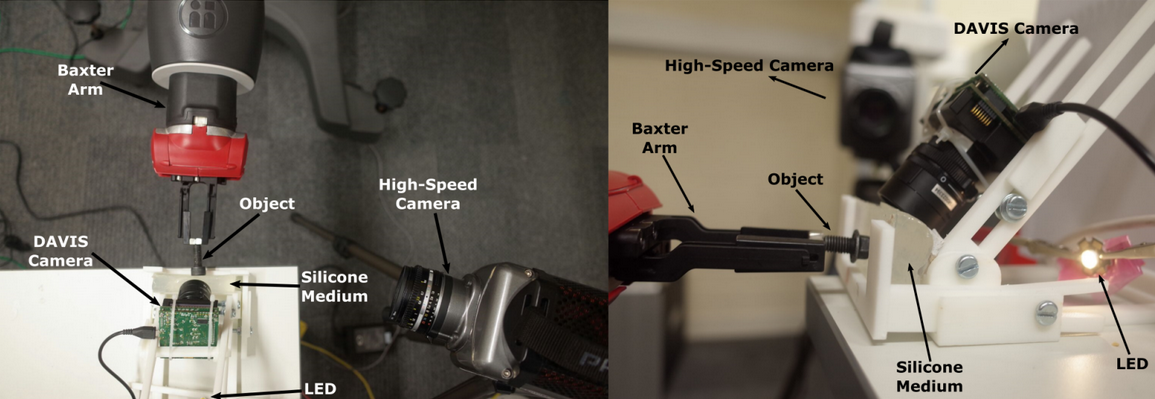
\includegraphics[width=\textwidth]{resources/images/rigi2018}
    \caption{Top-down (left) and sideways (right) views of the experiment setup ~\cite{rigi2018}.}\label{fig:rigi2018}
\end{figure}

Muthusamy et al. \cite{muthusamy2020slip} presents a first study on using an event-based camera with narrow field of view to detect slip during manipulation, but it analyzes only tiny motions. Moreover, it provides a slip suppression strategy regulating the grip force. The experimental setup is formed by the Baxter robot, electric parallel gripper, F/T sensor and a finger with an integrated event-based camera, as shown in ~\Cref{fig:muthusamy2020slip}. The F/T sensor measures six components of force and torque and is used only for validation purposes. In terms of the event-based camera, it observes the object through one of the transparent fingers of the gripper, which limits the information available from the object. The sensor itself moves attached to the gripper in this case, being suitable for pick-and-place operations.

\begin{figure}[h]
    \centering
    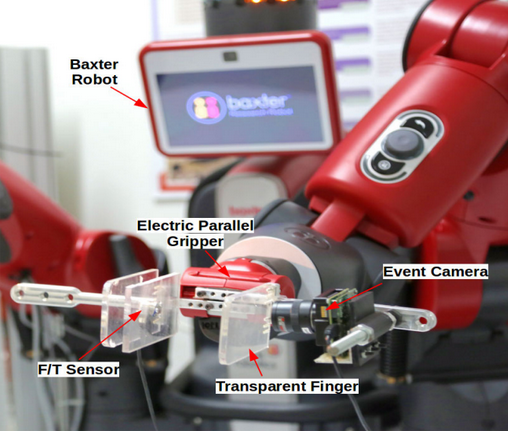
\includegraphics[width=0.7\textwidth]{resources/images/muthusamy2020slip}
    \caption{Experiment setup: Baxter Gripper with event-based finger prototype ~\cite{muthusamy2020slip}.}\label{fig:muthusamy2020slip}
\end{figure}

Another family of sensors widely used in the literature for slip detection are the tactile sensors, which may provide physical signals like the ratio of shear force to normal force, vibration or acceleration. In ~\cite{gelsight2017}, a tactile sensor, called GelSight sensor, is used for measuring geometry and detecting slip. Concretely, both translational and rotational slips are considered during grasp tasks, not complete pick-and-place operations. The GelSight sensor detects slip based on 3 major clues: the relative displacement between the objects and the sensor surface, the shear displacement distribution of the markers on the sensor surface and the change in the contact
area. They perform grasp experiments on 37 daily-use objects, lifting these slowly for 3 cm and then stopping. Each object is lifted 7 to 10 times, with different gripper forces, and the data is manually labeled indicating whether a slip occurred or not during the grasping and lifting process. Moreover, they implement a grasp closed-loop control with the feedback of the GelSight slip detection, using 33 objects and grasping each of them 3 times. If slip is detected the object is released and it is re-grasped with a higher gripping force.\\

In ~\cite{gelsight2018} the tactile information obtained from the GelSight sensor is combined with visual information coming from an external camera (standard webcam). The new setup including this camera is depicted in ~\Cref{fig:gelsight}. In this case a dataset is created including more than 1200 grasp experiments with 94 objects in total (for the train and test sets) and a deep neural network is trained to classify whether in a certain lifting sequence a slip has occured or not. These lifting sequences consider only small vertical motions with a non-textured (uniform) background and, in each grasp, the gripper width is modified in order to provoke slip or even complete failure in the grasp, which is manually annotated. They conclude that the best results are achieved combining tactile and vision information and, when using only vision information, much better results are achieved when the difference of images are taken into account, instead of the raw images. Note that using difference of images coming from a standard camera is a similar paradigm compared to event-based cameras, but these present a lower latency and therefore the feedback is faster.

\begin{figure}[h]
    \centering
    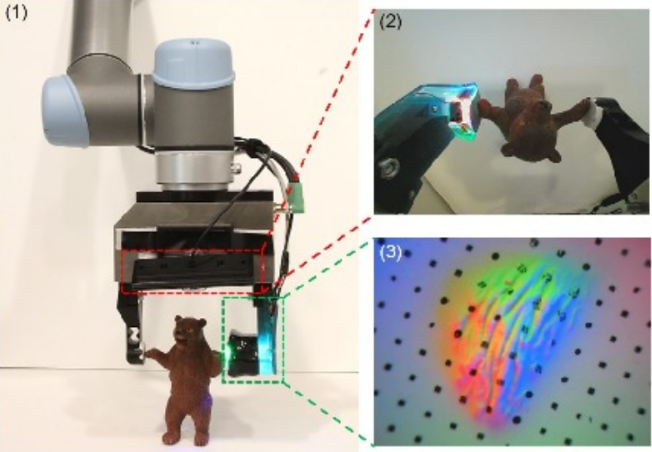
\includegraphics[width=0.7\textwidth]{resources/images/gelsight}
    \caption{(1) Experiment setup: UR5 robot arm with gripper, GelSight sensor and external camera. (2) Image captured by the external camera. (3) Image from GelSight sensor ~\cite{gelsight2018}.}\label{fig:gelsight}
\end{figure}

More work has been done in the combination of tactile and visual information, as in ~\cite{rss2020}, where they designed a Visual-Tactile Spiking Neural Network for rotational slip detection using their NeuTouch tactile sensor and the Prophesee event camera. In the experimental setup, see ~\Cref{fig:rss2020}, they also include 2 RGB cameras (for visualization and validation purposes), one mounted on the end-effector pointing towards the griper and the second one was placed to provide a view of the scene, and 11 OptiTrack cameras were used to collect ground-truth data. OptiTrack is a motion capture system that tracks the motion of some reflective markers attached to, in this case, the end-effector and the object. With this information the relative trajectory of the object with respect to the end-effector can be analyzed to determine whether the slip occurred or not. During the experiments they used a object built with Lego Duplo blocks with hidden masses. One variant was designed to be balanced at the grasp point and the second one, modifying the hidden masses, is unstable to induce rotational slip. Both variants are lifted by 10 cm off the table (in 0.75 s) and then holded, repeating this 50 times for each variant. However, the model was trained only during the first 0.15 s of the lifting phase, as they focus on early slip detection. Additionally, the background scene recorded by the cameras corresponds to a controlled black background.

\begin{figure}[h]
    \centering
    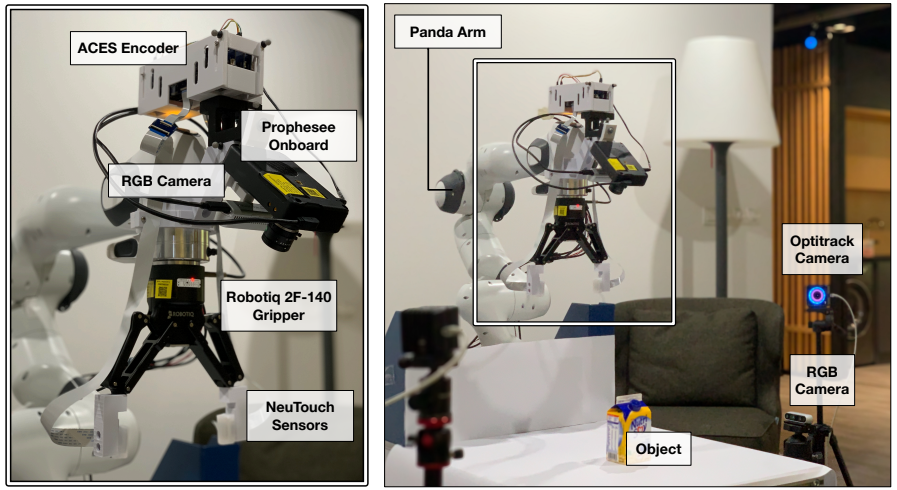
\includegraphics[width=0.95\textwidth]{resources/images/rss2020}
    \caption{Experiment setup: Robot arm, Prophesee event camera, Robotiq gripper, NeuTouch sensors, RGB and OptiTrack cameras ~\cite{rss2020}.}\label{fig:rss2020}
\end{figure}

\section{Conclusion}

Robot arms are widely used for pick-and-place motions and, combined with event-based cameras, which present several advantages compared to conventional frame cameras, they have the potential to form a robust manipulation and slip detection framework.\\

Even though there is some literature tackling this issue, none of them are considering the whole pick-and-place motion to detect slip and instead they are just analyzing tiny motions. Moreover, to make sure the solution generalizes the dataset should also include daily use objects and non-controlled background. When it comes to label the samples, some of the works determine if there is a slip or not by human inspection, however, ideally, having ground-truth data would be more suitable.\\

Most recent works are focusing on combining tactile and vision information, however, in industrial applications tactile sensors may have disadvantages like wear and a lack of long-term robustness. So, considering only visual information, concretely coming from an event-based camera, the placement of the camera in the end-effector should ensure a wide field of view, like in ~\cite{gelsight2018} and ~\cite{rss2020}.\\

In short, the topic of event-based vision for robot manipulation remains largely unexplored and thus offers great opportunities.\\

After having analyzed several experimental setups regarding robot manipulation with slip detection, in the next chapter our particular experimental setup is described.

    \cleardoublepage
\chapter{Experiment Setup}\label{sec:setup}

\section{Introduction}

The experiment setup consists of several existing components, like a robot system with its gripper, an event-based camera and a computer. However, to fix the event-based camera to the robot and gripper, a mount is needed, which has been designed according to our needs. Moreover, all these components are put together in a certain environment and using a certain software. Finally, due to the changes in the robot system (the addition of the mount and the camera) some adjustments have been made.

\section{Components}
\subsection{Robot system}

The robot system is composed by the robotic arm and controller, named Panda system, or simply Panda, which is a cobot developed and produced by the company Franka Emika GmbH.\\

The robotic arm has 7 DoF, where each axis is actuated through brushless DC motors, which are well-known for their high efficiency, high speed and no maintenance. In ~\Cref{fig:pandarobot} the axes of the arm are depicted as well as the work envelop of it.\\

\begin{figure}[h]
    \centering
    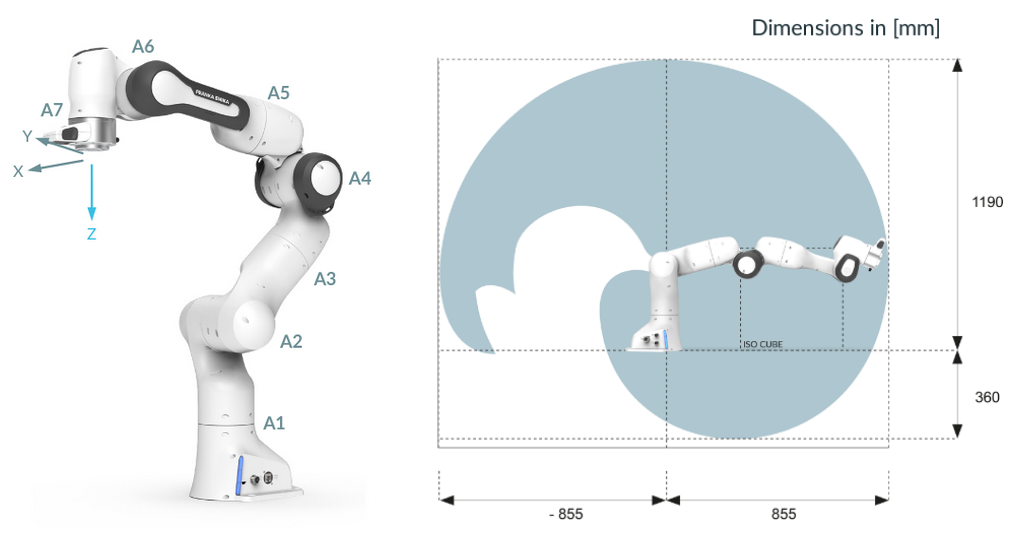
\includegraphics[width=\textwidth]{resources/images/pandarobot}
    \caption{Axes of the Panda robotic arm (left) and its work envelope (right) ~\cite{panda}.}\label{fig:pandarobot}
\end{figure}

The controller refers to the main control computer which is connected to the robotic arm and offers an Ethernet connection for a PC workstation. Additionally, the Panda system includes an emergency stop device integrated between the electricity connection and the controller. This device also enables the guiding mode, which consists of moving the robotic arm manually.

\subsection{Gripper}

The end-effector used for the pick-and-place operation is an electrical two-finger parallel gripper, shown in ~\Cref{fig:pandagripper}. This gripper is specifically designed for Panda, as it communicates directly via the connection in the robotic arm and is also supplied with power from it.

\begin{figure}[h]
    \centering
    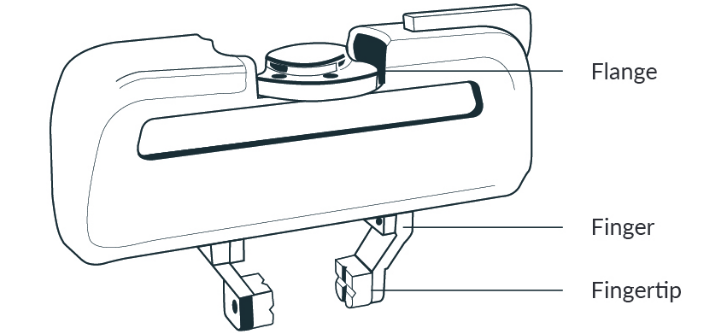
\includegraphics[width=0.6\textwidth]{resources/images/pandagripper}
    \caption{Two-finger parallel gripper ~\cite{panda}.}\label{fig:pandagripper}
\end{figure}

\subsection{Event-based camera}

The used event-based camera is the DAVIS 346, from iniVation, which provides as output not only the events, but also the grayscale frames. We use this camera with its lens, as shown in ~\Cref{fig:davis}.

\begin{figure}[H]
    \centering
    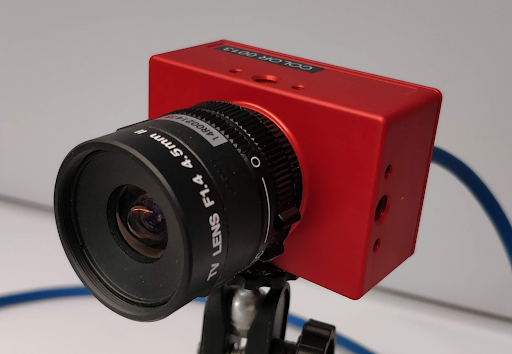
\includegraphics[width=0.4\textwidth]{resources/images/davis}
    \caption{DAVIS 346 event-based camera from iniVation.}\label{fig:davis}
\end{figure}

The DAVIS 346 ~\cite{davis} has a resolution of 346 x 260 pixels, for both events and frames. In terms of the event output, the dynamic range is 120 dB and the latency is 20 $\mu$s. On the contrary, the grayscale dynamic range is 56.7 dB and the maximum frame rate is 40 fps.

\subsection{Computer}

Finally, a computer is needed to connect to the control of the Panda via Ethernet and send commands to the robotic arm and also to connect the event-based camera and process its output.

\section{Design of the camera mount}

In order to assemble the event-based camera to the robotic arm and the gripper we need a camera mount, which has to be designed to make sure the camera has a wide view of the contact between the gripper and the object, such as in the works ~\cite{gelsight2018} and ~\cite{rss2020}. Moreover, this mount should be robust enough to hold the camera firmly, but at the same time being as lightweight as possible. Also, it should provide flexibility in order to be able to adjust the camera's position during the research phase, without having to build a new mount each time.\\

The mount consists of two parts: part A and part B, as shown in ~\Cref{fig:mount}. To design part A, firstly, the connection to the robotic arm and gripper should be considered. Actually, the mount can be fixed with a screw directly to the robotic arm, in the same way as the gripper is fixed. Moreover, in order to reduce vibrations during the movement of the robot, the mount follows the shape of the gripper, thus, providing more stability. Then, an extension is designed with an inclination, such that, once mounted, the camera points towards the gripper. Finally, note that some holes have been introduced to part A with the only aim of reducing the weight of it. In terms of part B, it attaches to DAVIS 346 and to the part A with some screws, providing flexibility when it comes to choose the distance at which the camera is placed. Concretely, the connections of the camera and part B to part A, can be regulated, such that the distance from the gripper's center to the lens (distance \textit{d} indicated in ~\Cref{fig:assembly}) ranges from 10.5 to 19.5 cm, having in total 7 positions separated by 1.5 cm.

\begin{figure}[H]
    \centering
    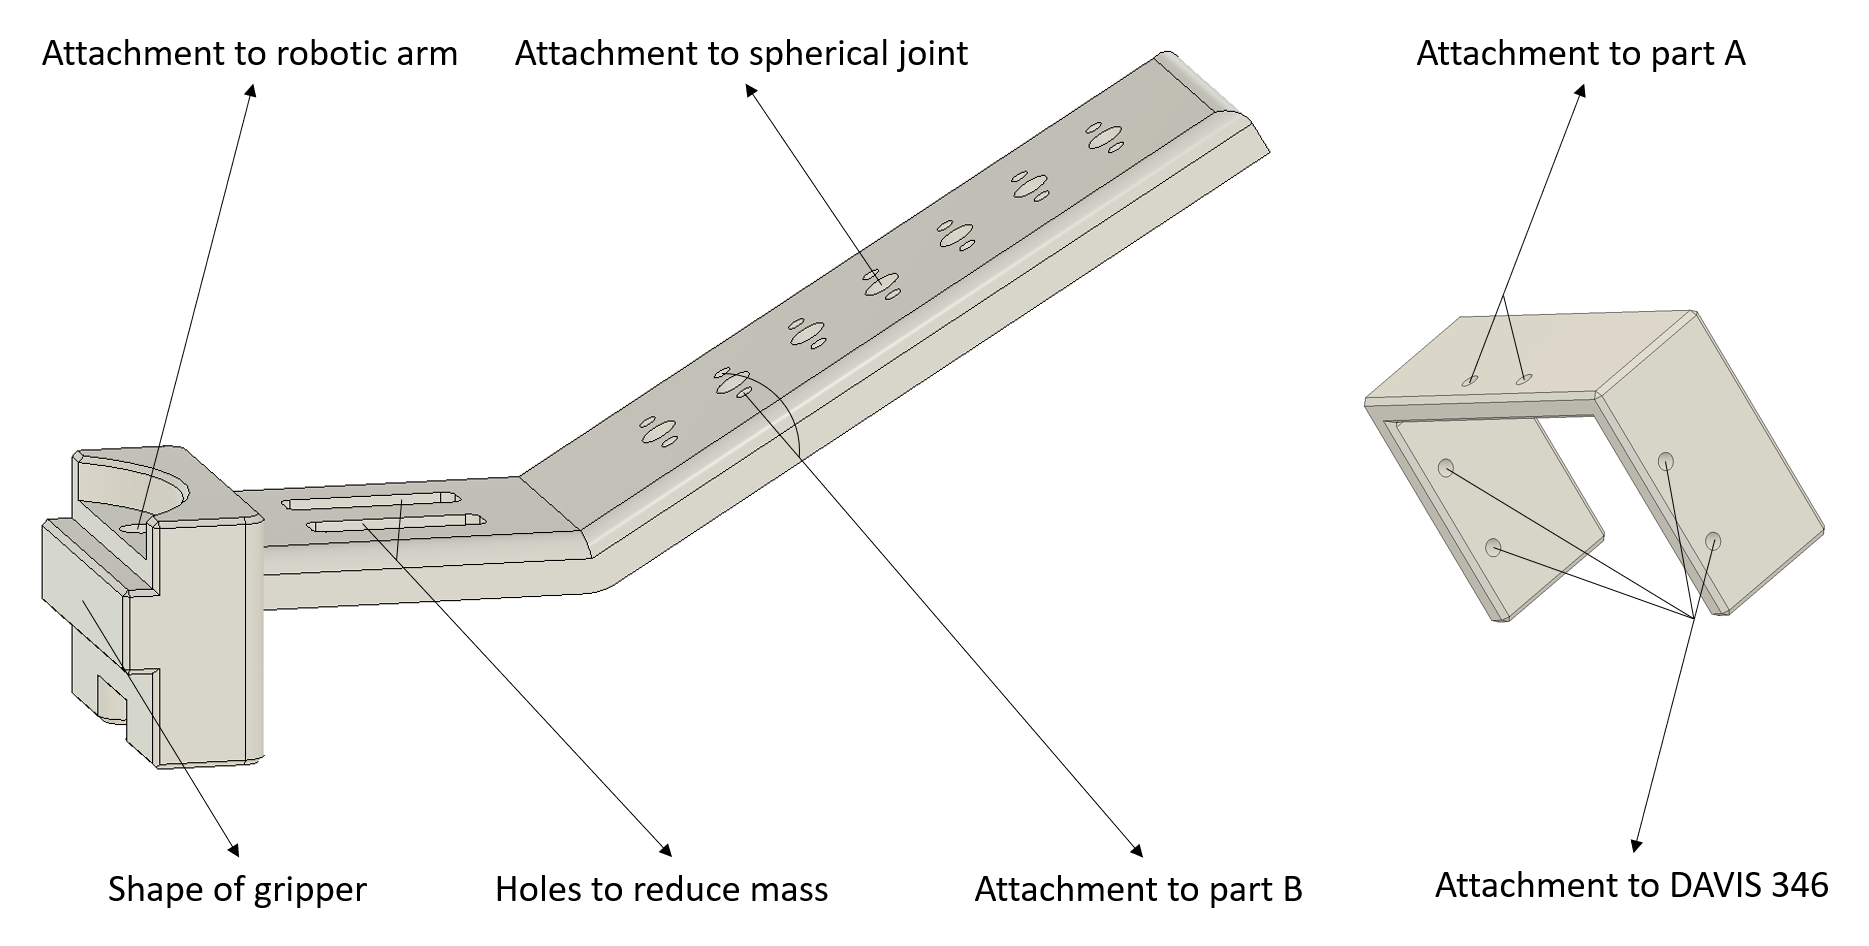
\includegraphics[width=\textwidth]{resources/images/mount_description}
    \caption{Description of the mount: part A (left) and part B (right).}\label{fig:mount}
\end{figure}

\begin{figure}[H]
    \centering
    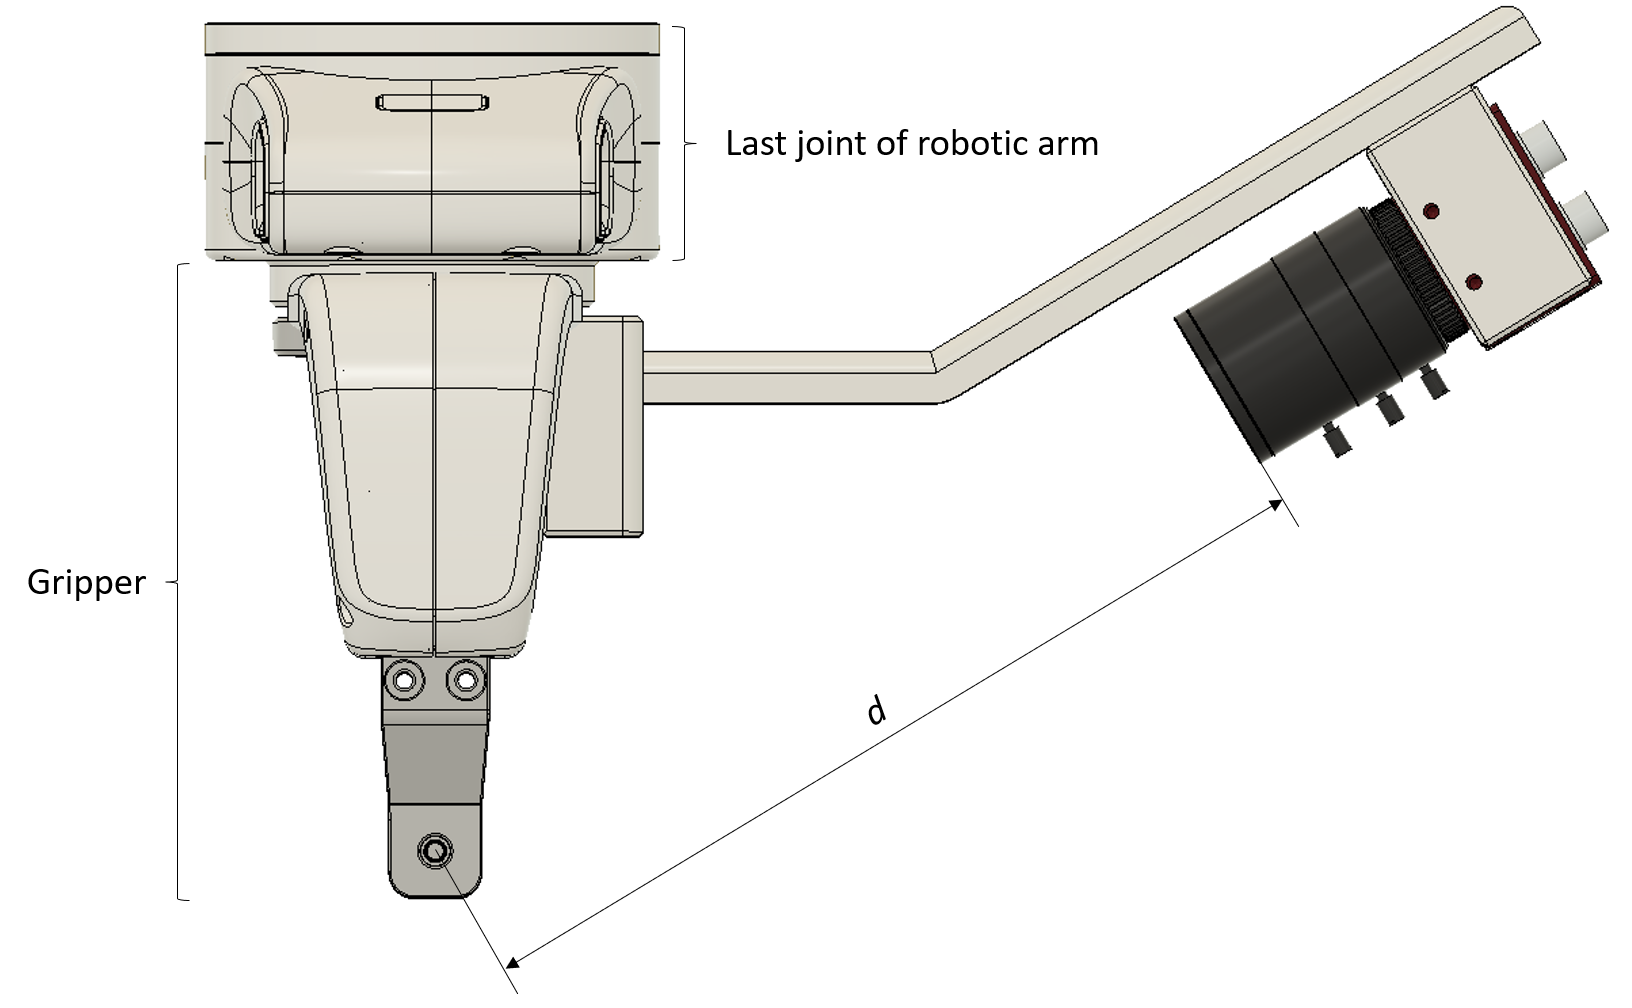
\includegraphics[width=\textwidth]{resources/images/assembly_description}
    \caption{Description of the assembly of the mount with the robotic arm, gripper and event-based camera.}\label{fig:assembly}
\end{figure}

In ~\Cref{fig:assembly} we can observe how all the components are assembled in CAD, and in ~\Cref{fig:assembly_real} the 3D printed mount, assembled with the robotic arm and the event-based camera, is shown.

\begin{figure}[H]
    \centering
    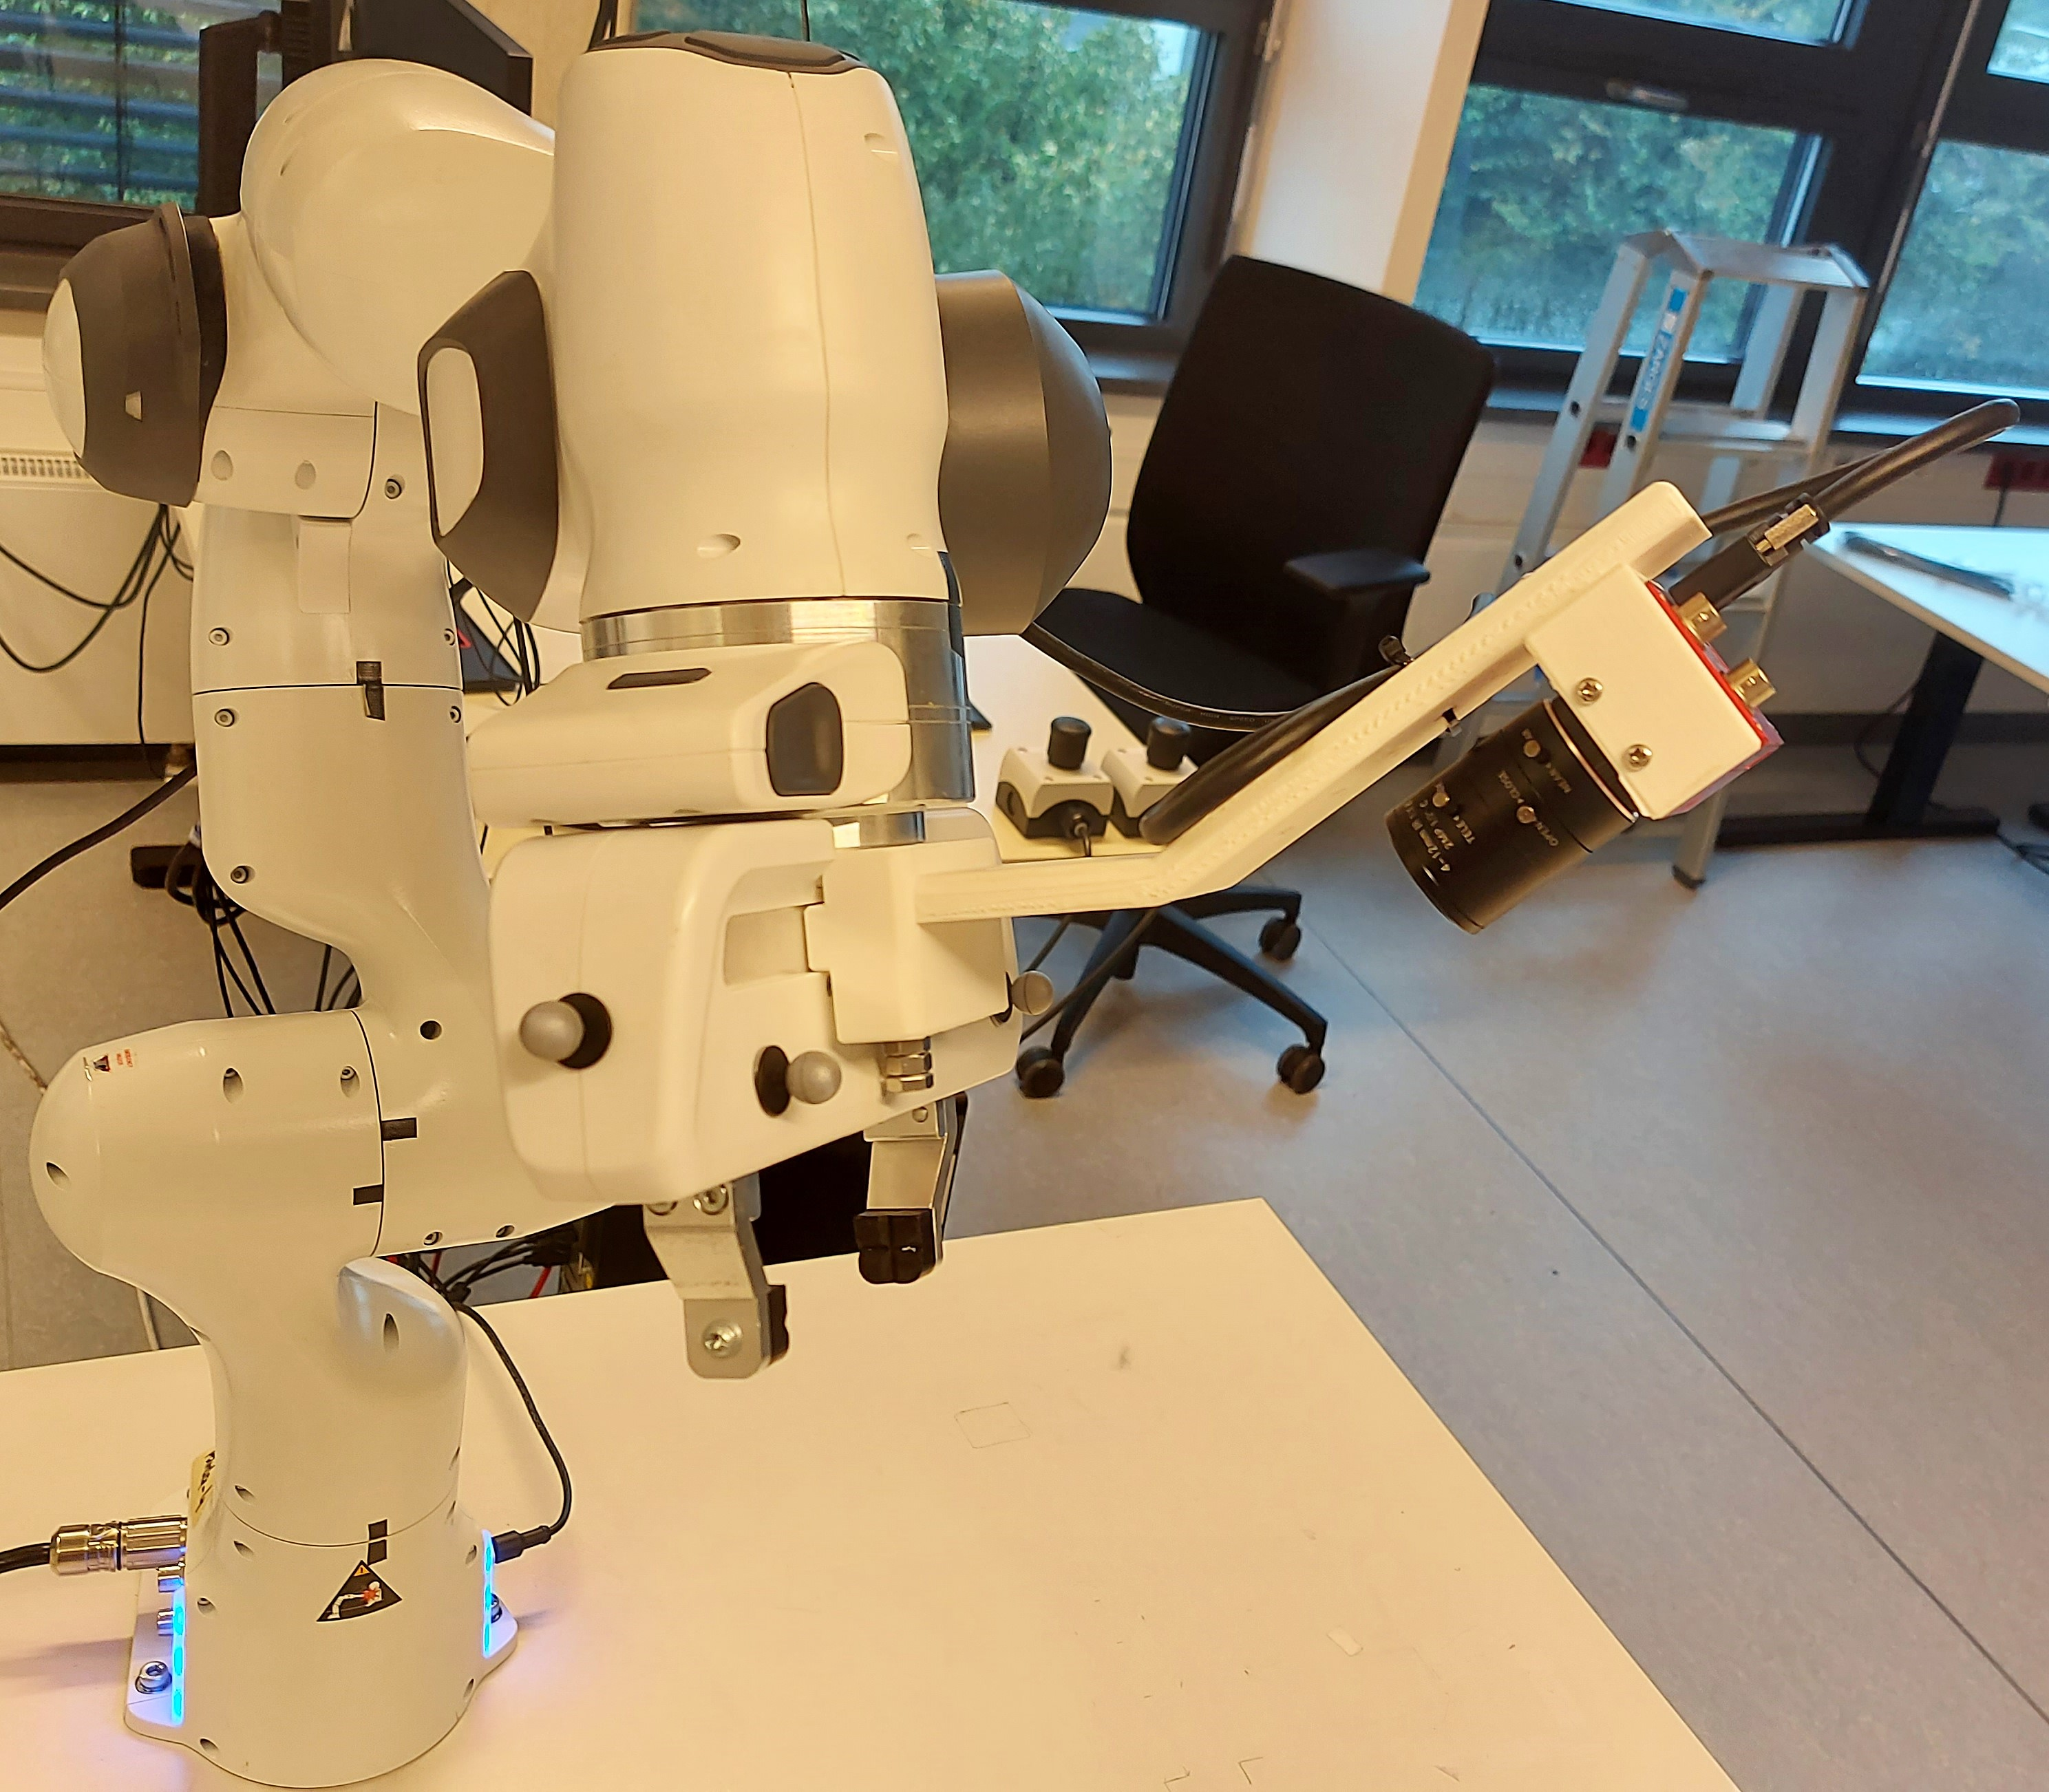
\includegraphics[width=0.85\textwidth]{resources/images/assembly_real}
    \caption{3D printed mount assembled with the robotic arm and event-based camera.}\label{fig:assembly_real}
\end{figure}

In addition, the camera can be connected to the mount using the spherical joint depicted in ~\Cref{fig:spherical}, using the holes provided in part A of the mount (see ~\Cref{fig:mount}). This joint enables the adjustment of not only the distance to the gripper, but also the orientation of the camera.

\begin{figure}[H]
    \centering
    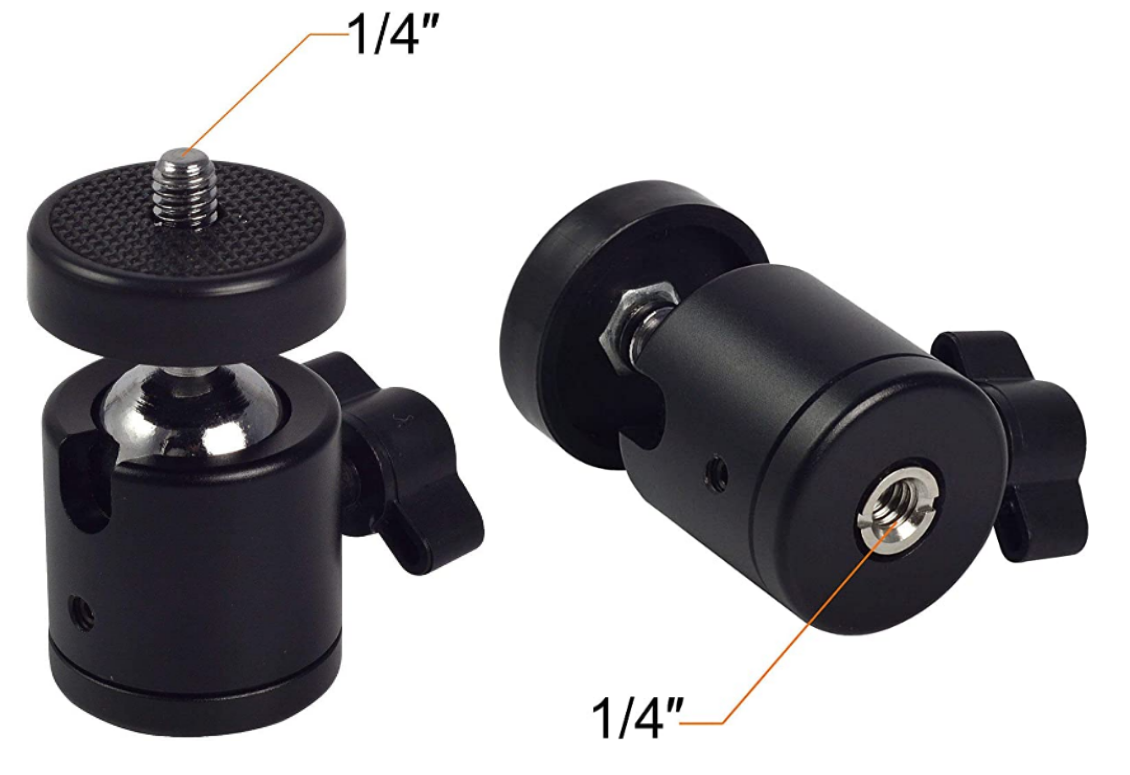
\includegraphics[width=0.6\textwidth]{resources/images/sphericaljoint}
    \caption{Spherical joint for cameras.}\label{fig:spherical}
\end{figure}

\section{Software}

\subsection{Required packages}

In order to control the robot arm and the gripper we use the \textit{botop}\footnote{\url{https://github.com/MarcToussaint/botop}} repository, which is used by the Learning \& Intelligent Systems (LIS) Lab at the TU Berlin.\\

To read and view the output provided by the camera DAVIS 346, we need the \textit{rpg\textunderscore dvs\textunderscore ros}\footnote{\url{https://github.com/uzh-rpg/rpg\textunderscore dvs\textunderscore ros}} package, which includes the C++ drivers and operates through Robot Operating System (ROS), a widely used framework for writing robot software.

\subsection{Developed code}

As the used setup and our needs differ from the ones of the LIS Lab, we needed to introduce some changes to the code and add some features to the existing \textit{botop} repository, creating a new repository\footnote{\url{https://github.com/MarcToussaint/co-ara/tree/ros_wrapper}} built on top of the aforementioned. Concretely, the trajectory was tuned, so that it was abrupt in the beginning to induce slip and ROS functionalities were added in order to be able to publish, and afterwards record, the information available inside the code.

\section{Calibration}

First, it is really important to configure the end-effector characteristics, as we are no longer using only the known two-finger gripper, but also the camera mount and the DAVIS 346. When configured incorrectly, gravitational forces are not entirely compensated and the robotic arm may pull towards certain directions in guiding mode, the regulation in operating mode may be affected so that the expected sensitivity of the arm for collision detection is reduced and the tracking behavior may be affected.\\

The new mass of the end-effector can be easily determined as the weight of all the elements (gripper, event-based camera and its mount with the screws) is known. However, the cable connected to the DAVIS 346 may introduce some slight changes. In terms of the center of mass and the inertia tensor, they were estimated using the CAD model of the elements (without considering the screws nor the cable) as a first estimation. Afterwards, using the command line tool \texttt{bot -float}, provided by the \textit{botop} repository, we could set the robot in a floating mode, where initially, if not configured properly, the robot tends to compensate the gravitational forces and move. So, by trial and error, the mass and center of mass were fine-tuned until the robot stayed still in the floating mode.\\

Also, to compute the trajectory, a collision checking is performed, however, the existing models in \textit{botop} repository are no longer valid, as the camera and its mount may collide with the table when grasping the object. Thus, the configuration file should be modified accordingly, resulting in the model shown in ~\Cref{fig:collision}. Finally, a frame is added to the camera lens, so that its pose and velocities are available.

\begin{figure}[H]
    \centering
    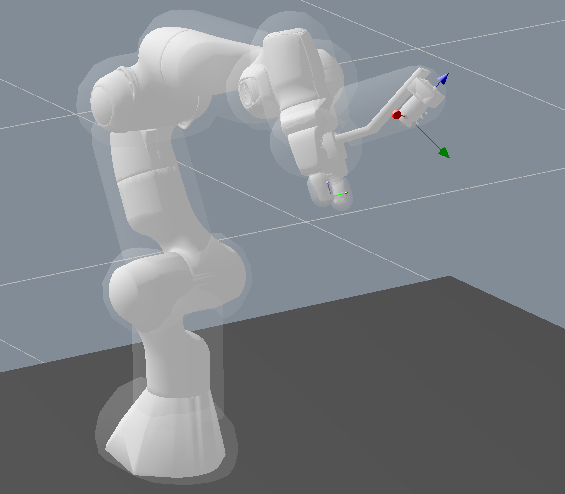
\includegraphics[width=0.7\textwidth]{resources/images/collision}
    \caption{Robot model including gripper with the camera and its mount.}\label{fig:collision}
\end{figure}

\section{Conclusion}

All in all, the described elements form the experiment setup, shown in ~\Cref{fig:setup}. As one may notice, the robot arm is placed above a white table, where the pick-and-place of the object is executed.

\begin{figure}[H]
    \centering
    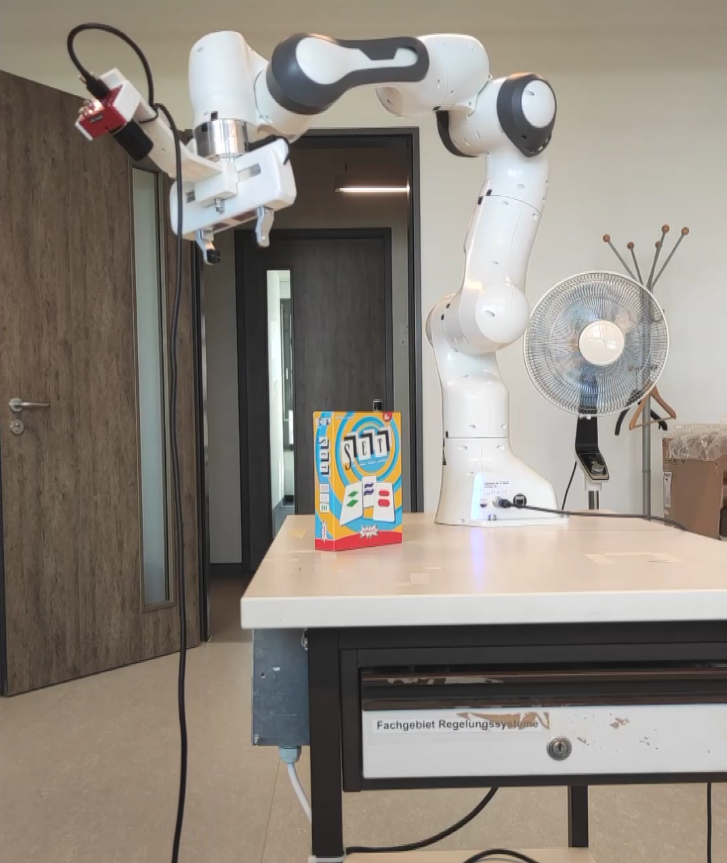
\includegraphics[width=0.8\textwidth]{resources/images/setup}
    \caption{Experiment setup: robotic arm, gripper, event-based camera and its mount.}\label{fig:setup}
\end{figure}

Using this setup, we were able to record data of slip and non-slip scenarios in different phases. After each recording phase, the data was analyzed, new requirements were noticed and new data was collected taking these into consideration. The results of the data collection are presented in the following chapter.

    \cleardoublepage
\chapter{Data Collection}\label{sec:data}

\section{Introduction}

The output of the DAVIS camera is the main source of information. On the one hand, we have the grayscale frames @40 Hz. On the other hand, the events are generated asynchronously and are saved with their pixel location, polarity and timestamp. Therefore, some kind of representation is needed to visually inspect the data. For this purpose the events are represented using event images, where the events are accumulated for a certain time window (30 ms in our case) and a pixelwise histogram of events is built, generating a 2D image. Usually, pixels with gray color mean that no events occurred in the current time window, whereas different shades of white indicate positive polarity and shades of black indicate negative polarity. Event images have an intuitive and informative interpretation, as events are caused by moving edges, these frames are like edge maps and edges convey a lot of information of a scene. Moreover, if the object does not slip, it will not move, as its relative pose with respect to the camera does not change, thus no events will be generated due to the motion (only some events may be generated due to illumination changes) and no edges will be visible in the event images. On the contrary, if the object slips we will be able to see edges in the event images.\\

Using the experiment setup described in the previous chapter, we can start to record data of pick-and-place motions. Concretely, in ~\Cref{fig:rob_traj} we can observe a sequence of images of a complete pick-and-place motion executed by Panda with the assembled DAVIS 346. The images \textit{a-c}, show the reaching phase, where no slip needs to be detected. Specifically, in \textit{c} the gripper closes and the movement with the object starts, ending at image \textit{e}, and it is between these two instances where slip has to be detected, if it occurs. Finally, the object is released and the arm returns to the home position (\textit{f}). It is worth noticing that the relative position of the object with respect to the gripper changes significantly between image \textit{c} and images \textit{d} and \textit{e}, meaning that a slip occurred during the lifting phase.\\

\begin{figure}[h]
    \centering
    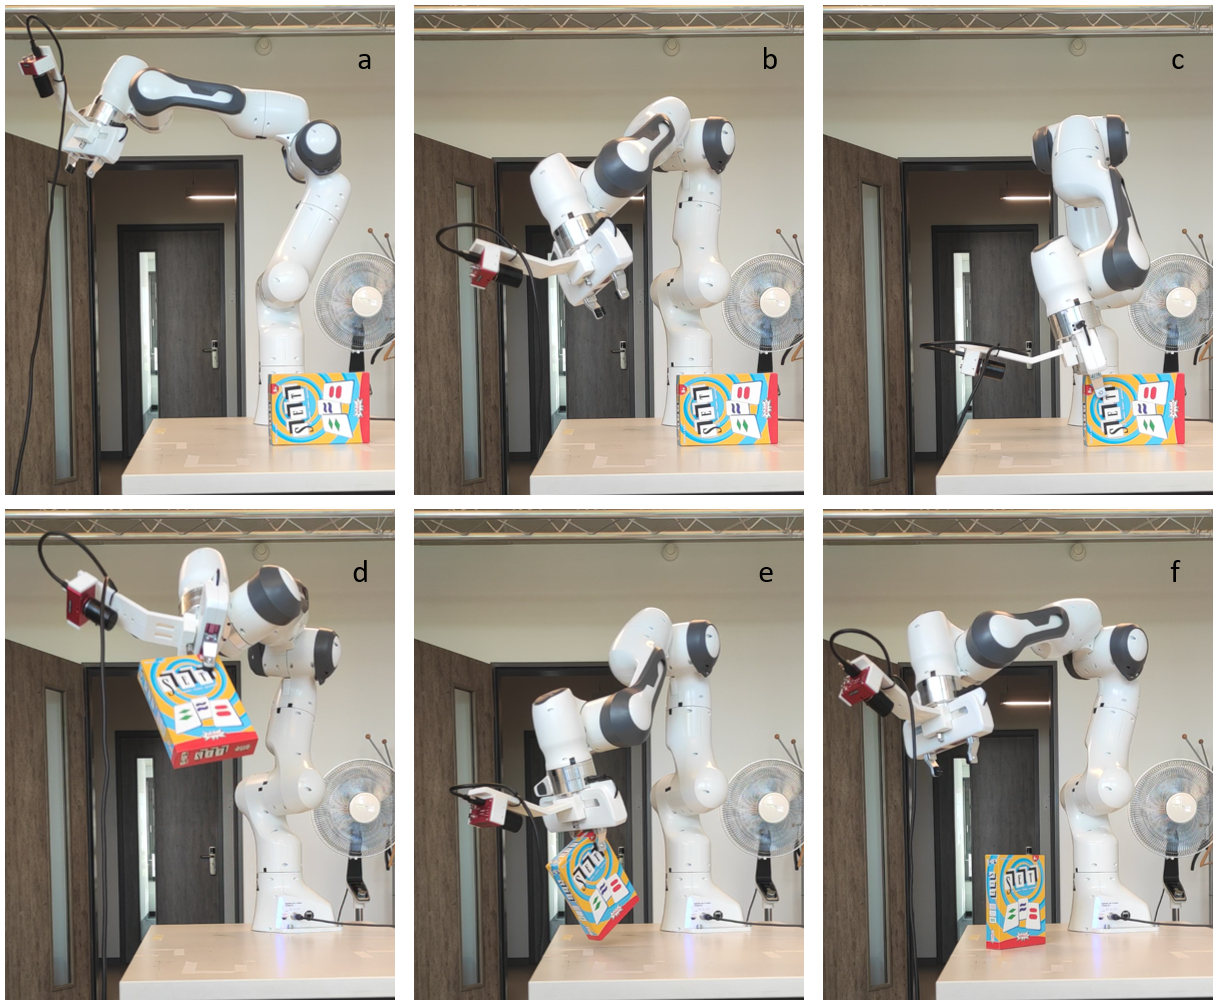
\includegraphics[width=\textwidth]{resources/images/rob_traj}
    \caption{Sequence of images (\textit{a-f}) showing an example pick-and-place motion.}\label{fig:rob_traj}
\end{figure}

During the experiments, a non-controlled background was present and textured objects were used in order to make sure events are generated if a slip occurs. This condition is not so strict, as most of the daily use objects have enough texture.\\

The first experiments were conducted with the goal of exploring different kinds of slip and grasp failures, with diverse objects. Then, we focused our efforts on a concrete type of slip and recorded more data. Furthermore, we recorded additional data in different scenarios including more sources of information into the dataset, which were required to explore other methods for slip detection.

\section{Initial data}

First, we had to think about how to generate slip or grasping failures during a pick-and-place motion. For that, in the literature, either the gripper's force is modified ~\cite{gelsight2017}, so that if it is not enough it will induce slip or grasp failure, or the gripper's width is modified ~\cite{gelsight2018}, so that if it is too wide the object will not be picked properly. However, we realized that the two-fingered gripper designed for Panda, that we are using, has a minimum force of 20 N, which is already enough to grasp and move lightweight objects and even heavy objects grasped from the center. Moreover, the gripper width has a binary behavior, either it closes until the indicated gripping force is reached, or it does not even close. Therefore, the only option to generate slip experiments by changing the gripper's force and/or width is by changing the gripper itself, for example, the Robotiq 2F-85 or 2F-140 would be suitable. Nevertheless, the acquisition of such gripper and redesign of the camera mount would require a significant amount of time, which is out of the time frame of this thesis.\\

So, some other options to induce slip or grasping failures have been found, as described in the following subsections.

\subsection{Off-centered grasping}

In ~\cite{rss2020} slip is generated by grasping the object away from its center of mass, which will induce some rotation in the object during the lifting phase, as happened in the sequence shown in ~\Cref{fig:rob_traj}.\\

A first slip sequence is shown in ~\Cref{fig:init_exp1}, where a heavy book is grasped from the corner, away from its center of mass. In the first event image, we can observe the edges of the two fingers of the grippers, as it is closing. Also some edges of the object are visible due to some movement provoked by the gripper. In the following two frames, events appear in the background, as the arm with the attached camera are moving, and from the object, due to rotational slip. It is worth noticing that there are no events coming from the end-effector and part of the camera mount, as they move rigidly with the camera, hence there is no difference in the pixels during the whole motion. Finally, once the slip stops, there are no more events coming from the book, which starts also moving rigidly with respect to the camera, as happens in the last frame.

\begin{figure}[h]
    \centering
    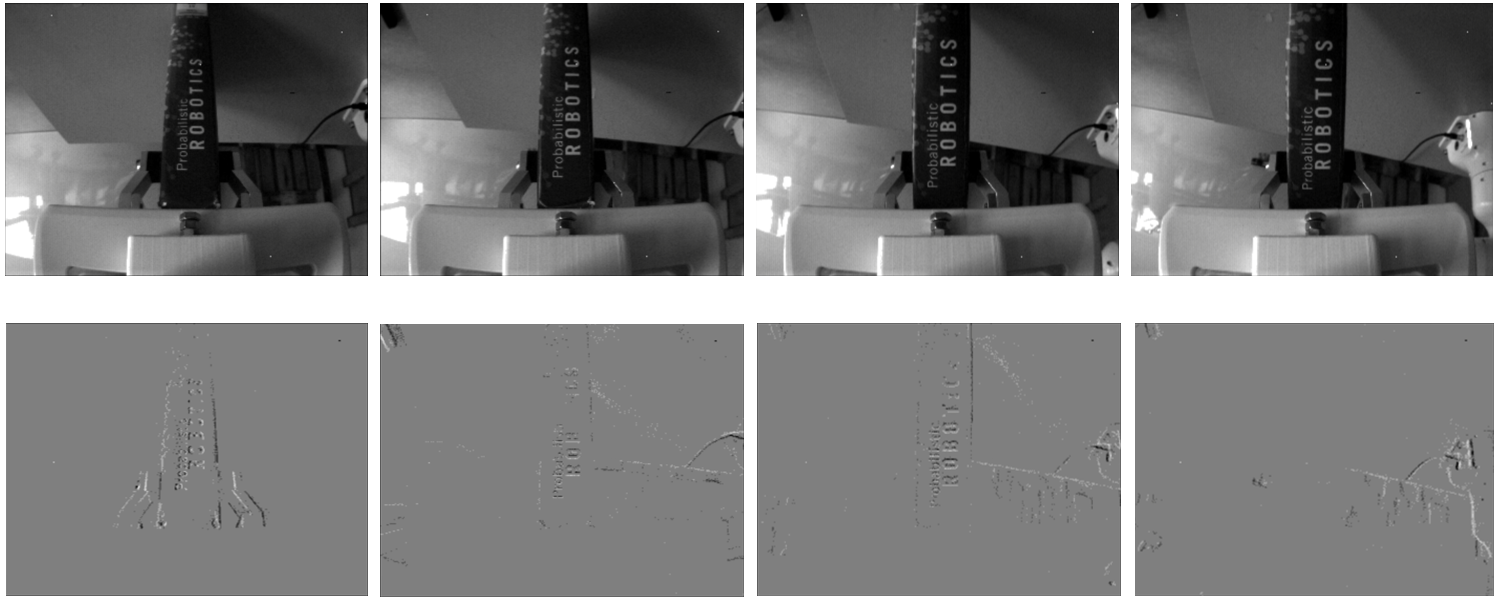
\includegraphics[width=\textwidth]{resources/images/init_exp1}
    \caption{Sequence of grayscale frames (first row) and event images (second row) during a slip, while executing a pick-and-place motion with a book.}\label{fig:init_exp1}
\end{figure}

Another sequence of off-centered grasping is depicted in ~\Cref{fig:init_exp2}, where a hammer is grasped from the bottom of its handle, having the center of mass quite far from the gripper, because of the weight of its head. Due to the high momentum generated while lifting the hammer, the object starts to swing fastly and it slips away from the gripper, provoking a grasping failure, as observed in the last frame. Again the event images are really informative of this failure, as events come and form a map of moving edges indicating the relative movement of the hammer with respect to the camera. As expected, there are also events coming from the background and, in the last frame, events come also from the two fingers of the gripper, because they close when the object slips through the fingers.

\begin{figure}[H]
    \centering
    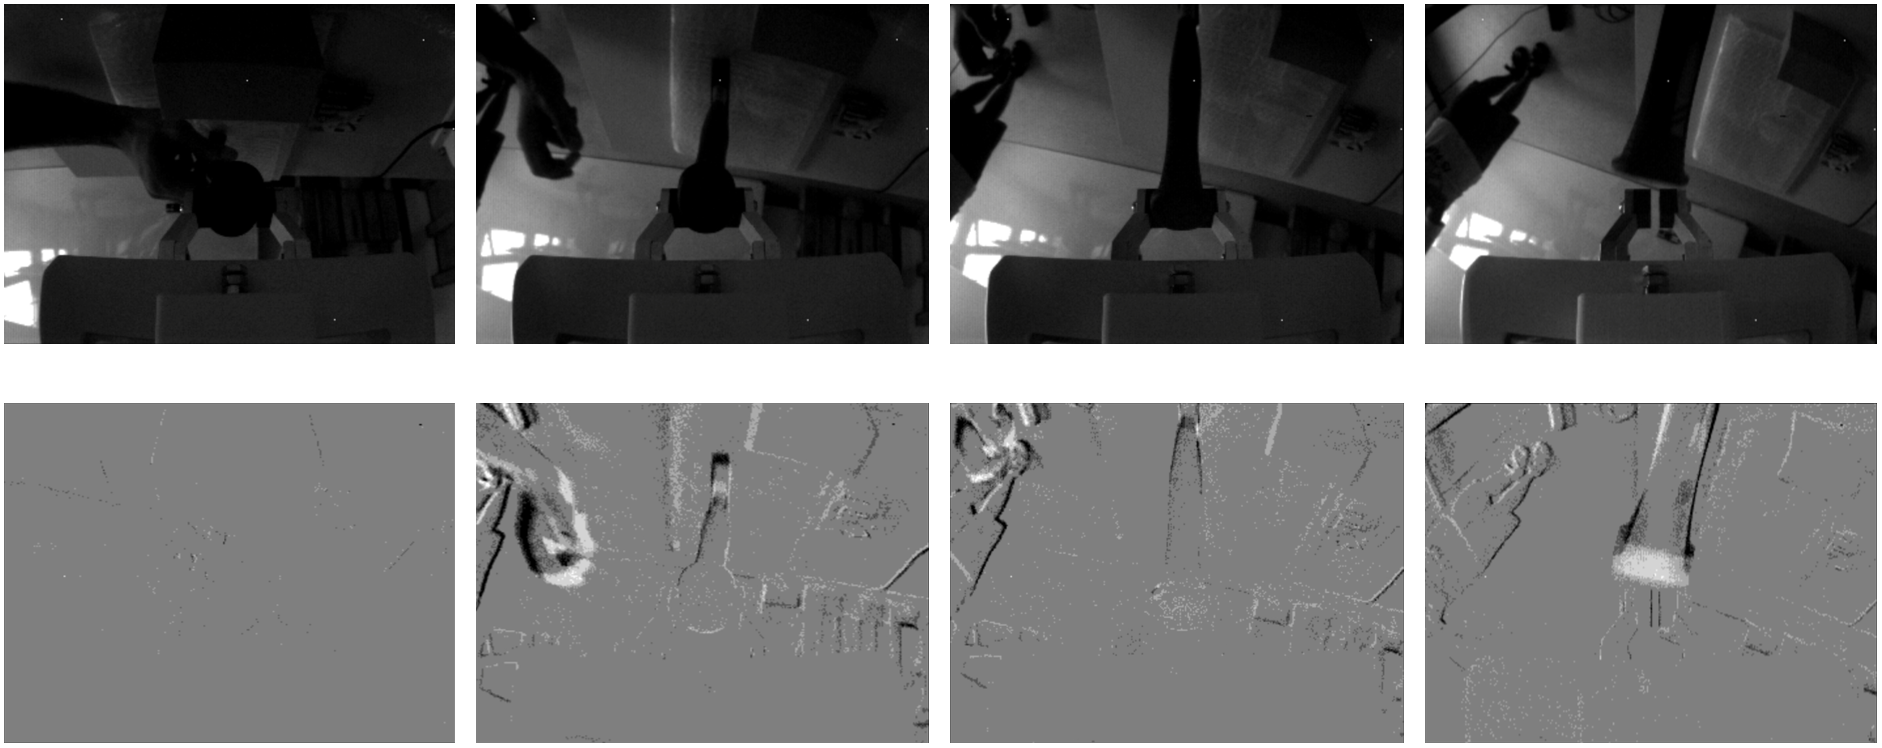
\includegraphics[width=\textwidth]{resources/images/init_exp2}
    \caption{Sequence of grayscale frames (first row) and event images (second row) during a grasp failure, while executing a pick-and-place motion with a hammer.}\label{fig:init_exp2}
\end{figure}

\subsection{Pulling with string}

An alternative way of forcing rotational slip, is by attaching a string to the object and pulling it, applying force to the object and forcing it to rotate. This might seem a synthetic scenario, but actually it resembles a real case where an object is picked in a cluttered environment and maybe the grasped object is attached to another object and gets pulled by it.\\

An example sequence is represented in ~\Cref{fig:init_exp3}, where first the object is pulled upwards (downwards in the images as they are inverted), generating the moving edges in the second event image. Then the object is pulled downwards (upwards in the images), with a clearly visible movement in the third event image. Finally, there are no more slips and no more events appear from the object in the fourth event image.

\begin{figure}[H]
    \centering
    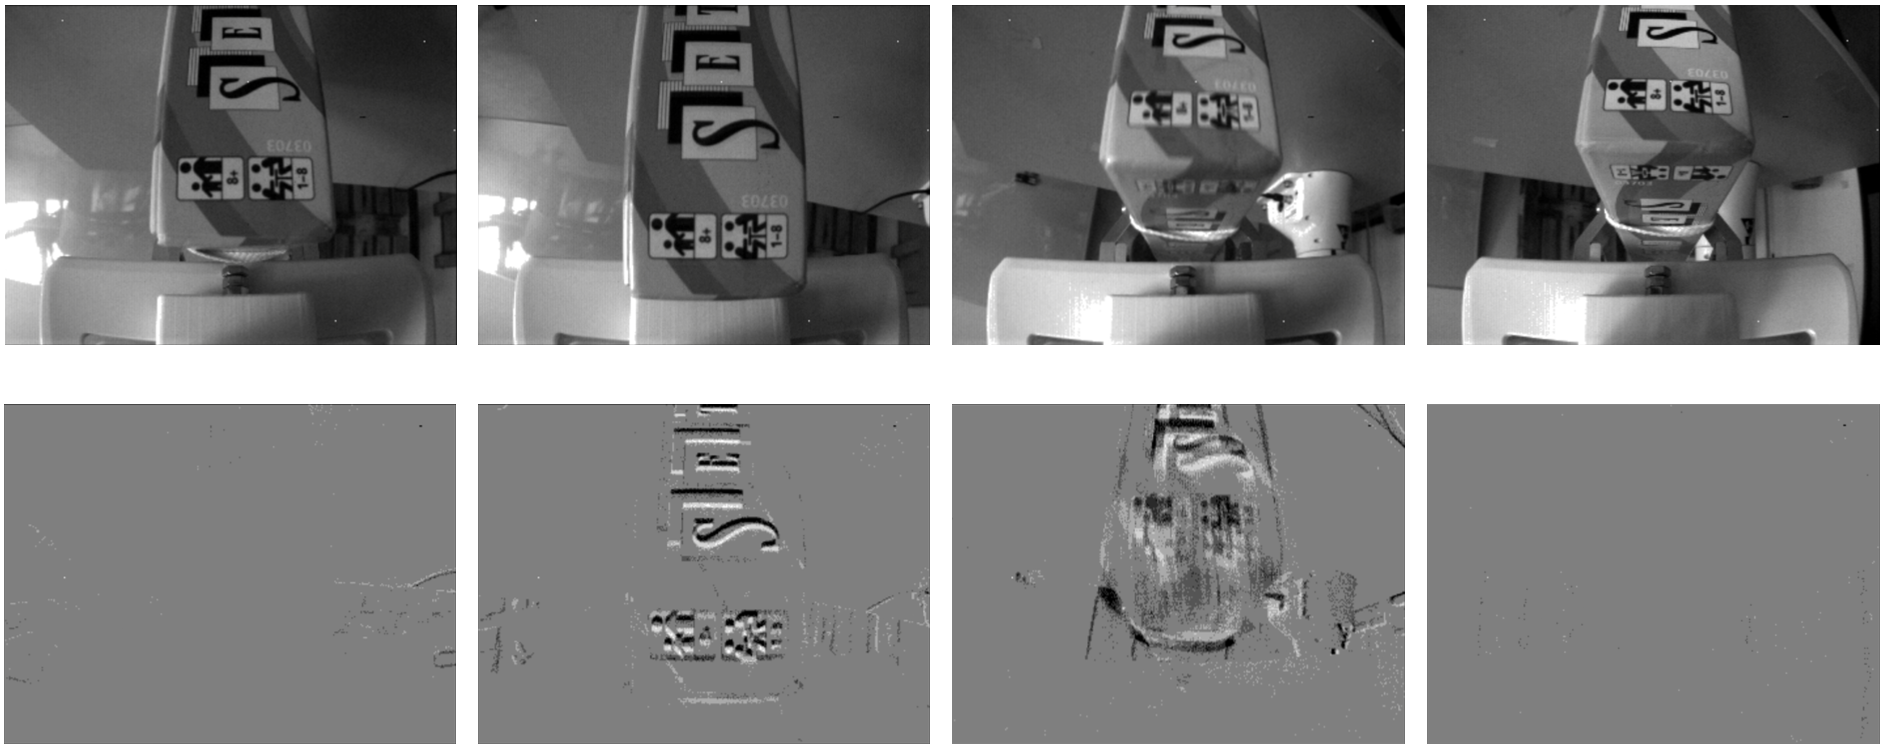
\includegraphics[width=\textwidth]{resources/images/init_exp3}
    \caption{Sequence of grayscale frames (first row) and event images (second row) during two slips generated by an external force, while executing a pick-and-place motion with a box.}\label{fig:init_exp3}
\end{figure}

\subsection{Deformable objects}

Until now only rigid bodies have been considered, however, instead of grasping the book as in ~\Cref{fig:init_exp1}, we can grasp some of its pages and the object will behave as a non-rigid body. In ~\Cref{fig:init_exp4} an example sequence is shown with this scenario, where we can observe how the book opens after lifting it and the non-grasped part of the book swings during the whole motion, which is visible through the edges of the book in the event images. Nevertheless, this is not a slip nor a grasping failure, it is a continuous swinging of part of the object, which may be useful to detect as it may damage it.

\begin{figure}[H]
    \centering
    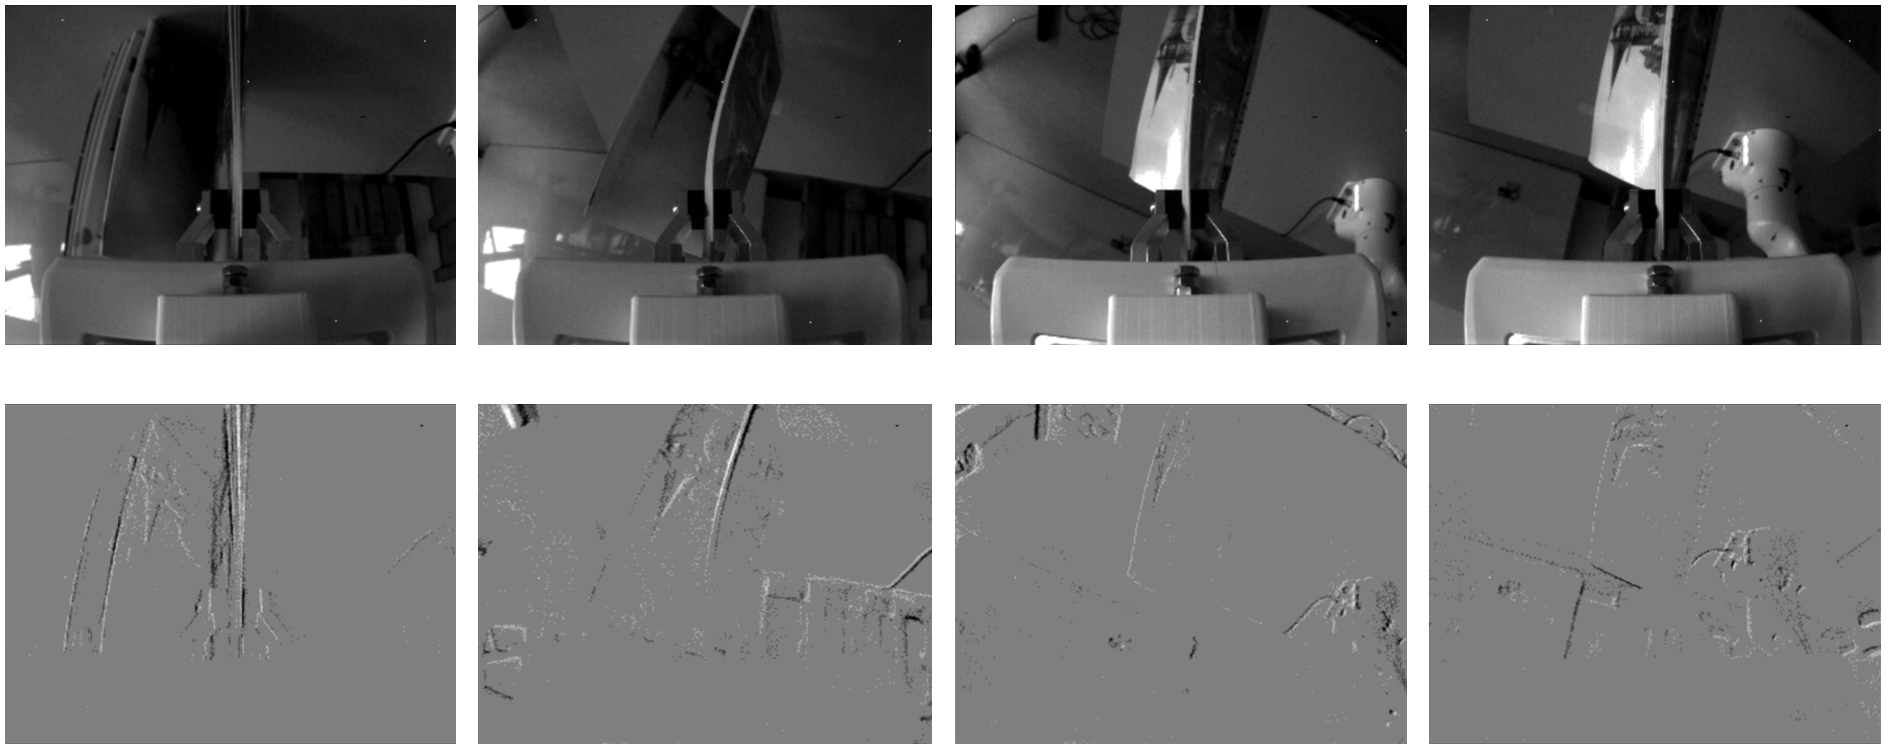
\includegraphics[width=\textwidth]{resources/images/init_exp4}
    \caption{Sequence of grayscale frames (first row) and event images (second row) during swinging, while executing a pick-and-place motion with an open book.}\label{fig:init_exp4}
\end{figure}

\section{Set 1}

After analyzing different ways of generating slip and grasping failures, we focused our efforts in studying in deep off-centered grasping using rigid bodies. This kind of grasping generates rotational slip in the beginning, which can be detected and the object can be placed again in the initial position and re-grasped from another point to make sure the pick-and-place motion occurs without slippage.\\

In ~\Cref{fig:set1_case1} a first example sequence can be observed, with a box which has a heavy mass inside in the other side of the grasping point, in order to induce slip. However, in this case there is only a slight rotation of the object, which can be appreciated thanks to the edges of the second event image.

\begin{figure}[H]
    \centering
    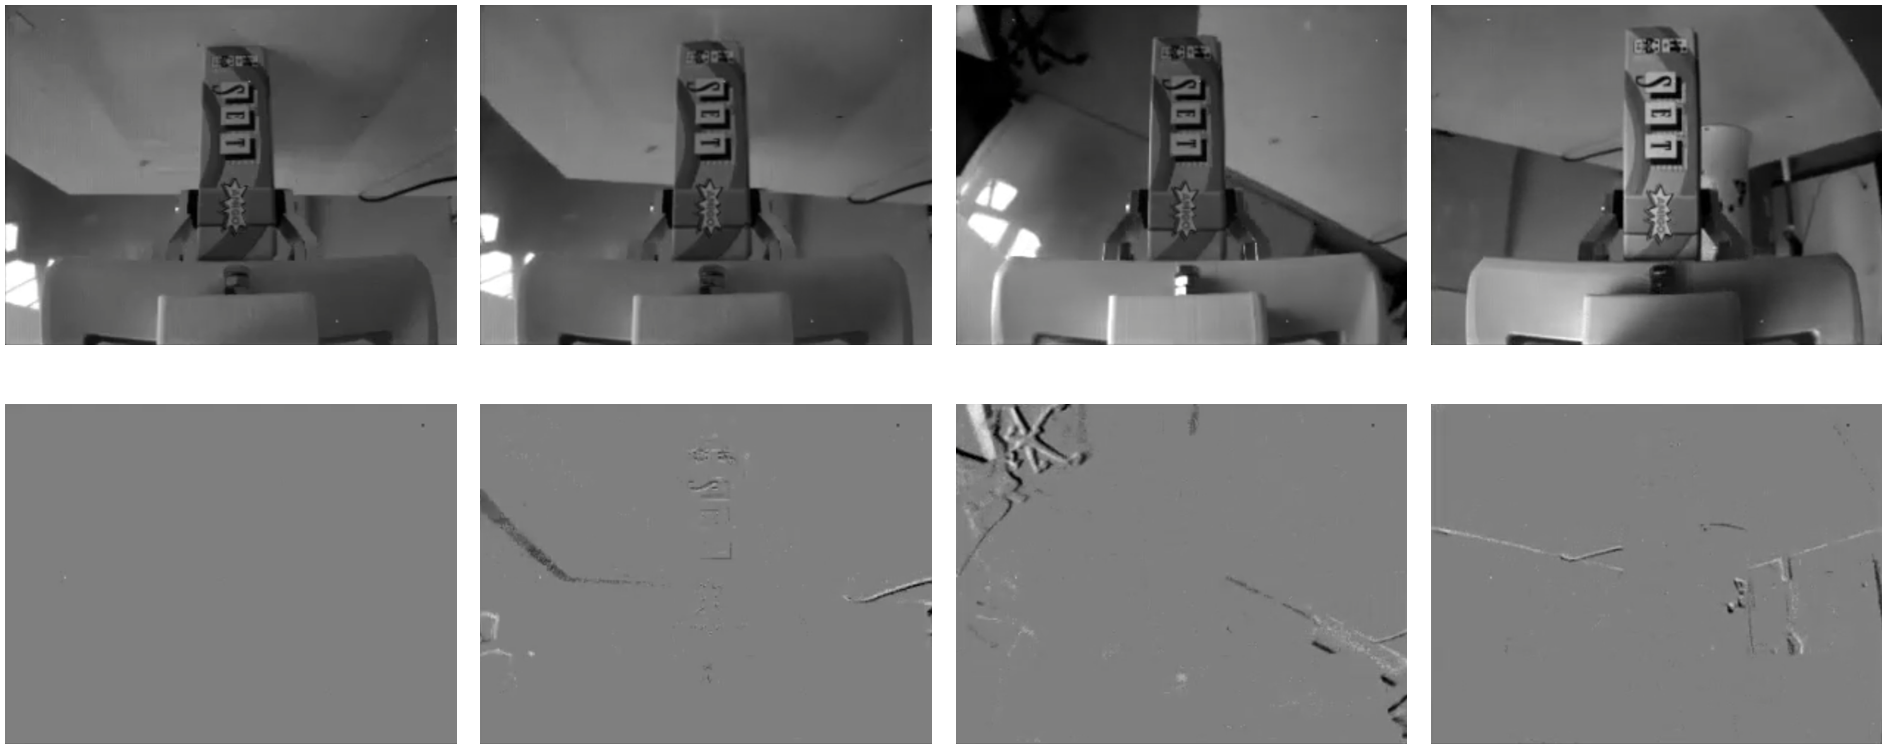
\includegraphics[width=\textwidth]{resources/images/set1_case1}
    \caption{Sequence of grayscale frames (first row) and event images (second row) during a minor slip, while executing a pick-and-place motion with a box.}\label{fig:set1_case1}
\end{figure}

On the contrary, in ~\Cref{fig:set1_case2}, a significant slip occurs in the same scenario, varying slightly the grasping point. First, the object rotates in one direction, as observed in the second frame, and then it rotates in the opposite direction, which can be appreciated in the third frame. To see the direction of rotation by looking at the event images, we can focus on the letter \textit{S}, which is black over a white background. If the \textit{S} moves downwards, as happens in the second frame, the pixels below will change their value from white (high value in grayscale) to the black pixels (low value in grayscale) of the letter \textit{S}, generating events with negative polarity (represented with black shades in the event image). Oppositely, the pixels in the \textit{S} change from black to white, generating events with positive polarity (represented with white shades in the event image). In contrast, in the third frame the event polarities are switched with respect to the previous frame, therefore, the \textit{S} is moving upwards, indicating a change in the direction of slip. Finally, the slip ends and the place motion is completed without additional slips, as there are no moving edges in the last frame.

\begin{figure}[H]
    \centering
    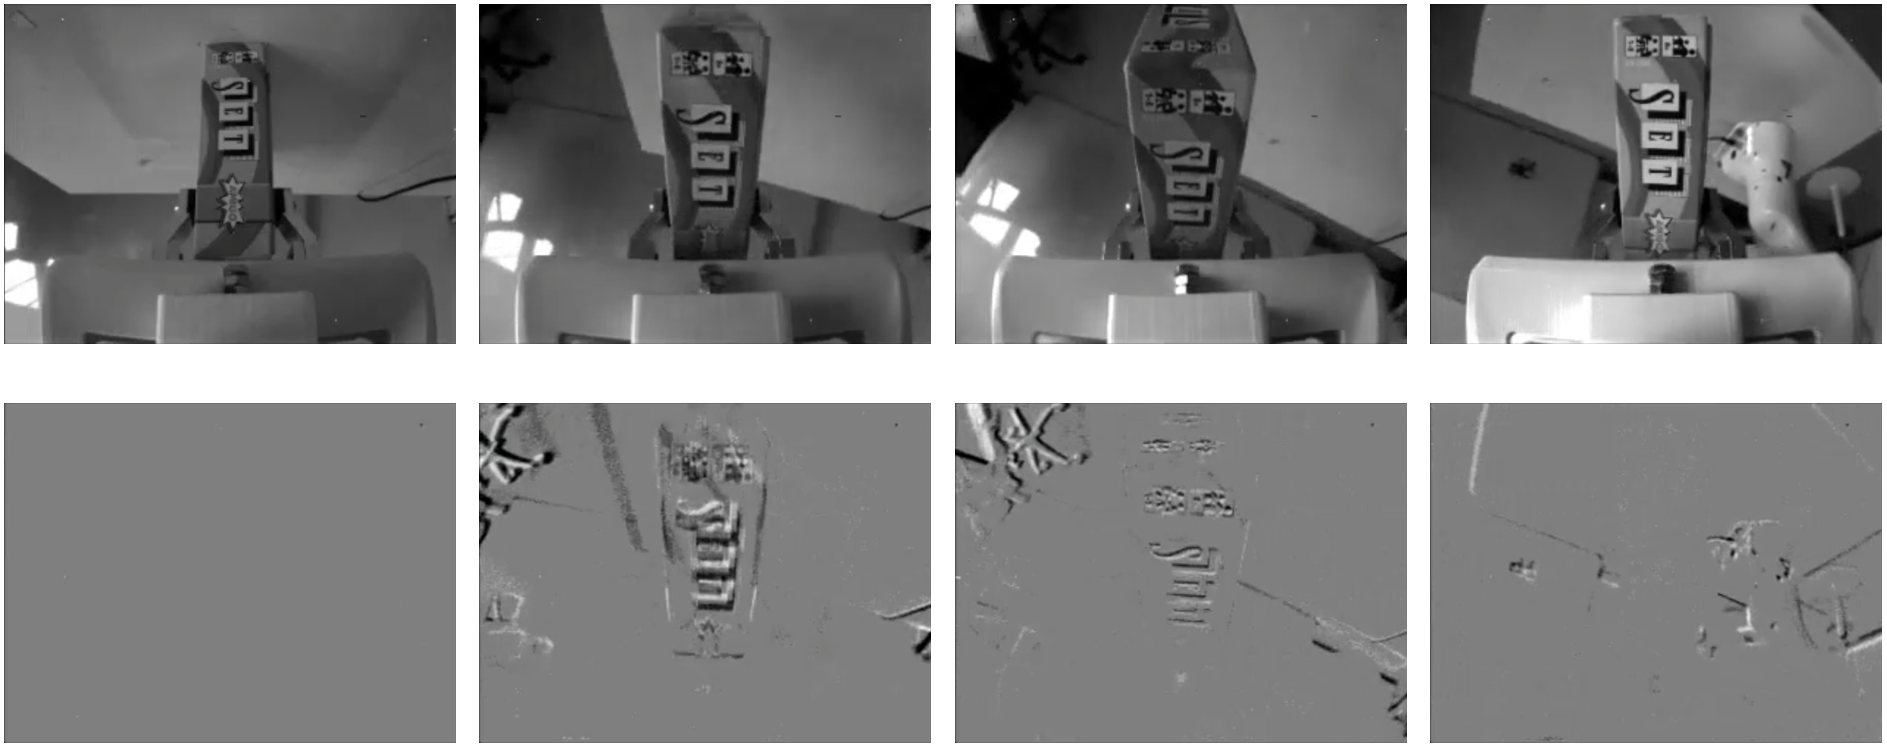
\includegraphics[width=\textwidth]{resources/images/set1_case2}
    \caption{Sequence of grayscale frames (first row) and event images (second row) during a significant slip, while executing a pick-and-place motion with a box.}\label{fig:set1_case2}
\end{figure}

Changing the object, and using instead a book, we can observe a similar behavior, as depicted in ~\Cref{fig:set1_case3}. In the second frame a slip is visible, thanks to the moving edges shown in the event image, which are generated by the letters on the book's cover. Then, in the third frame, the slip seems to stop, but the rotation continues to the other direction, as shown in the fourth frame. It is worth noticing that, if there were no letters on the cover, meaning no texture in the object, there would not be any events caused by the slips.\\

\begin{figure}[h]
    \centering
    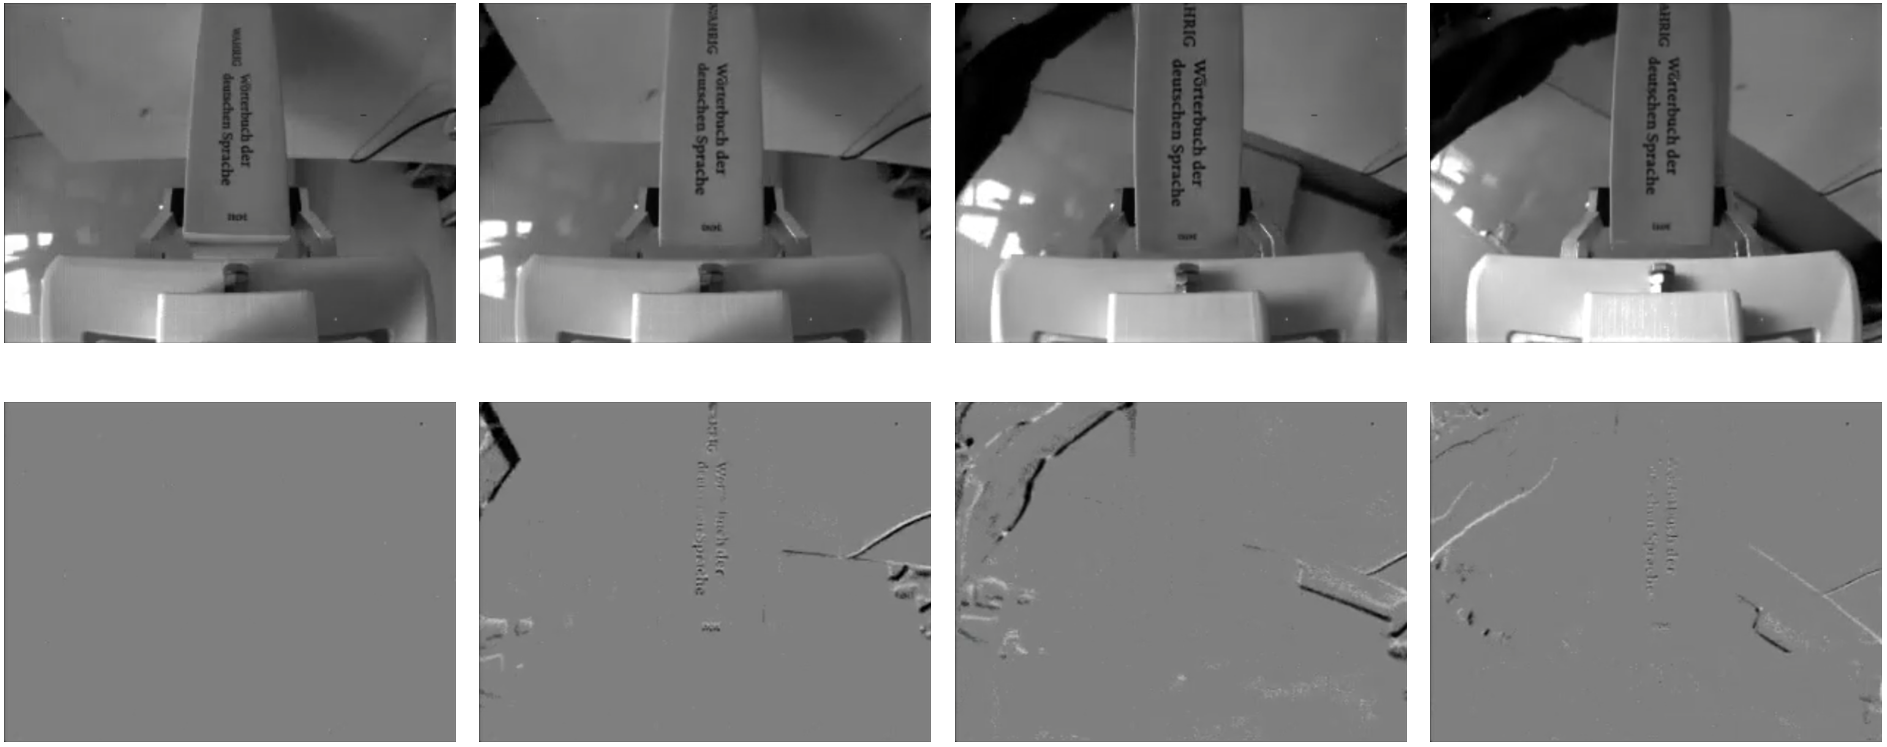
\includegraphics[width=\textwidth]{resources/images/set1_case3}
    \caption{Sequence of grayscale frames (first row) and event images (second row) during a significant slip, while executing a pick-and-place motion with book no. 1.}\label{fig:set1_case3}
\end{figure}

Using another book, with more texture, see ~\Cref{fig:set1_case4}, only one slip occurs in the second frame. Thanks to having more texture, the edges in the event image are more visible.\\

\begin{figure}[h]
    \centering
    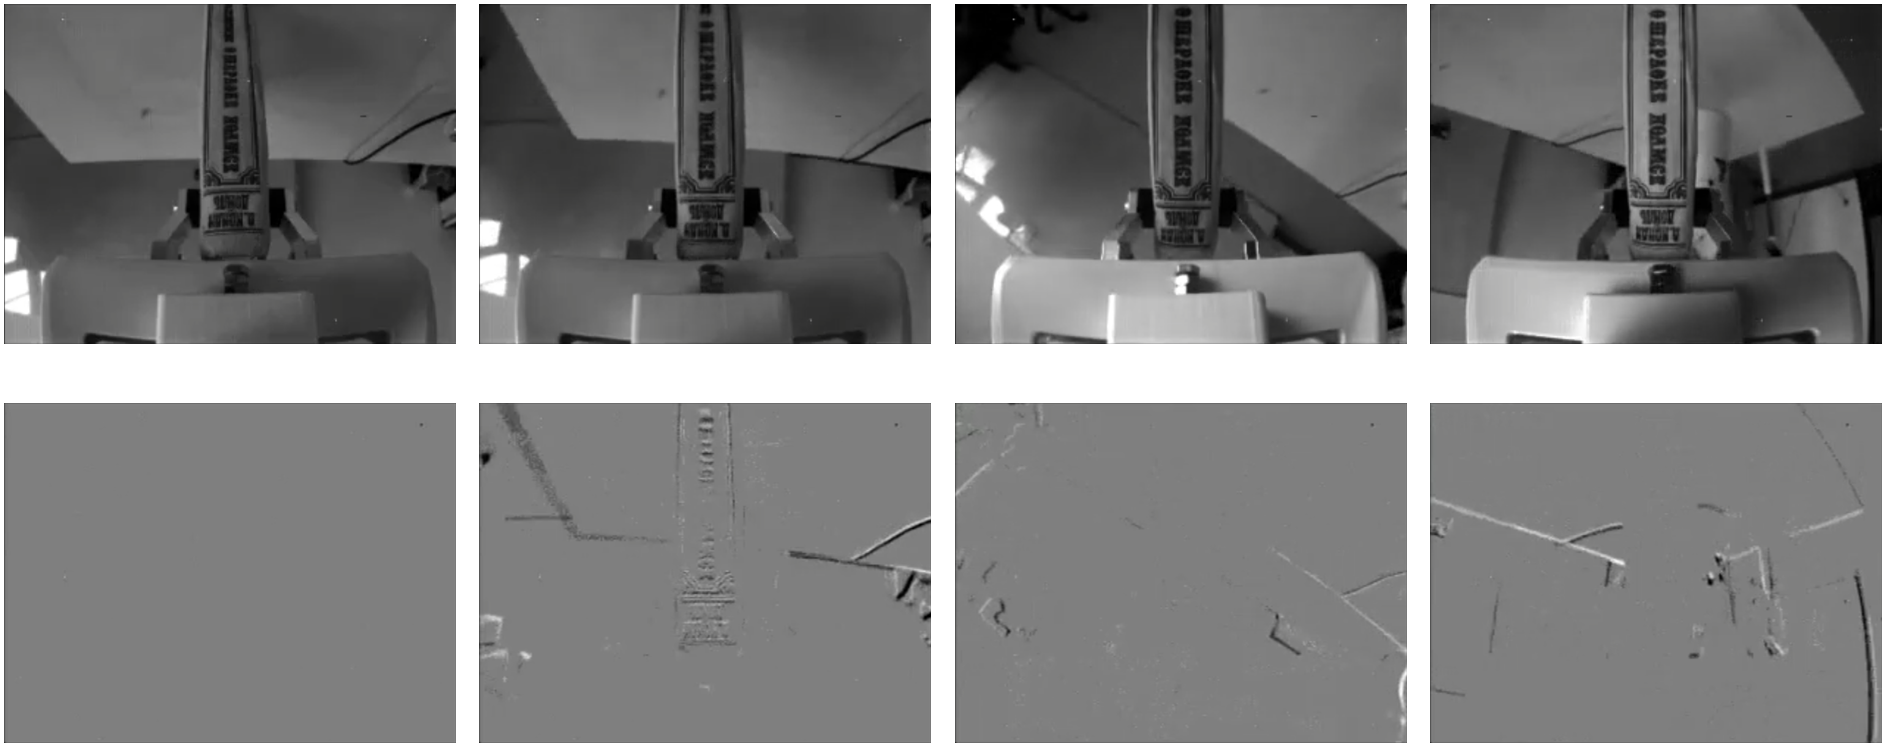
\includegraphics[width=\textwidth]{resources/images/set1_case4}
    \caption{Sequence of grayscale frames (first row) and event images (second row) during a significant slip, while executing a pick-and-place motion with book no. 2.}\label{fig:set1_case4}
\end{figure}

The same book, can be grasped just from the opposite side of it, so that the rotational slip occurs in the other direction. In ~\Cref{fig:set1_case5}, we can see the slip happening in the second and third frames. This experiment is relevant also to see the effects of having the object really close to the camera in the beginning of the motion.\\

\begin{figure}[h]
    \centering
    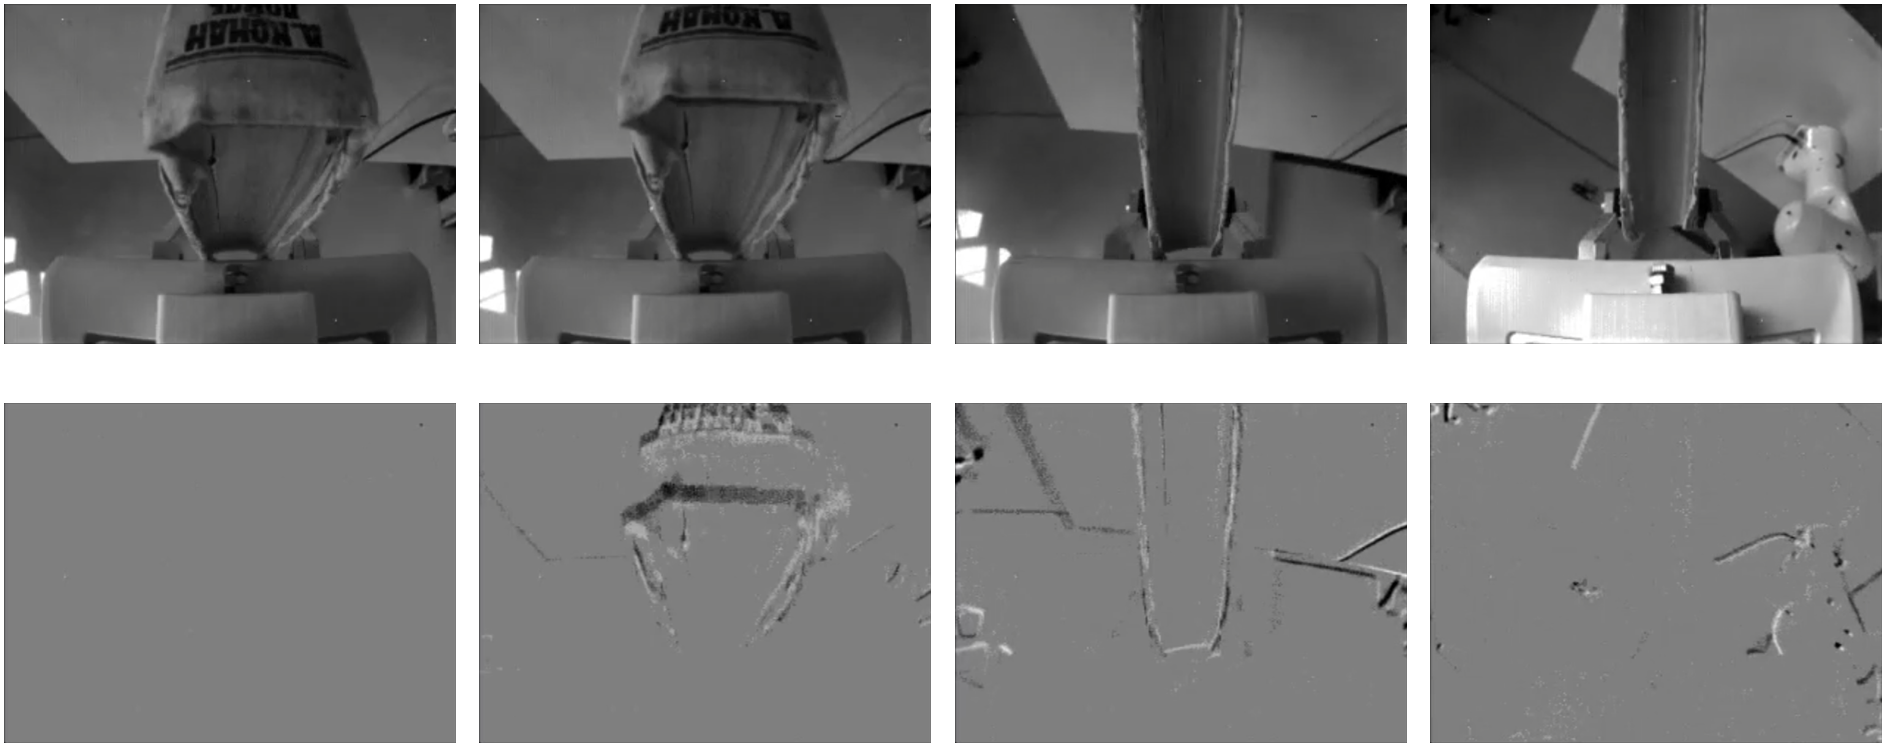
\includegraphics[width=\textwidth]{resources/images/set1_case5}
    \caption{Sequence of grayscale frames (first row) and event images (second row) during a significant slip, while executing a pick-and-place motion with book no. 2 and reverse grip.}\label{fig:set1_case5}
\end{figure}

This same scenario can be replicated with the box used in the first experiments, as shown in ~\Cref{fig:set1_case6}. The slip is similar to the previous case, but now more events appear, thanks to the highly textured object, and the box is even closer to the camera.

\clearpage

\begin{figure}[h]
    \centering
    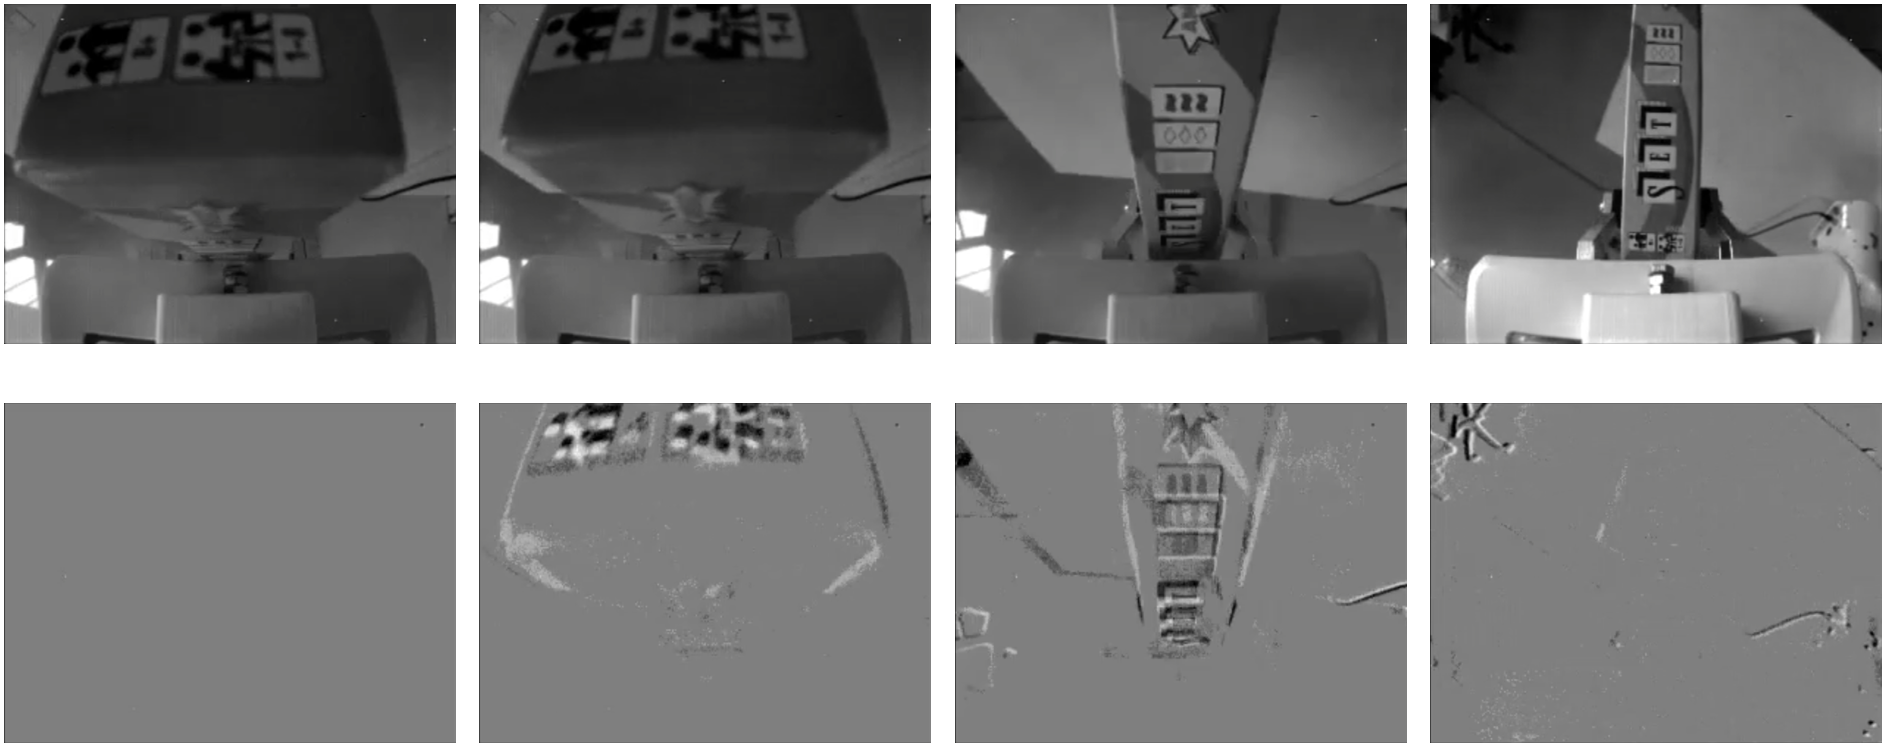
\includegraphics[width=\textwidth]{resources/images/set1_case6}
    \caption{Sequence of grayscale frames (first row) and event images (second row) during a significant slip, while executing a pick-and-place motion with a box and reverse grip.}\label{fig:set1_case6}
\end{figure}

Finally, the book used in ~\Cref{fig:set1_case3} is used again but changing the texture of the background. Concretely, a mat of photos has been placed on the table. In ~\Cref{fig:set1_case7}, the resulting sequence is shown, where the events coming from the book are similar compared to ~\Cref{fig:set1_case3}, but the background has many more moving edges in the event images. It is quite important to try also different background scenarios, to make sure that the developed methods do generalize in such conditions, or at least to know their limitations.

\begin{figure}[H]
    \centering
    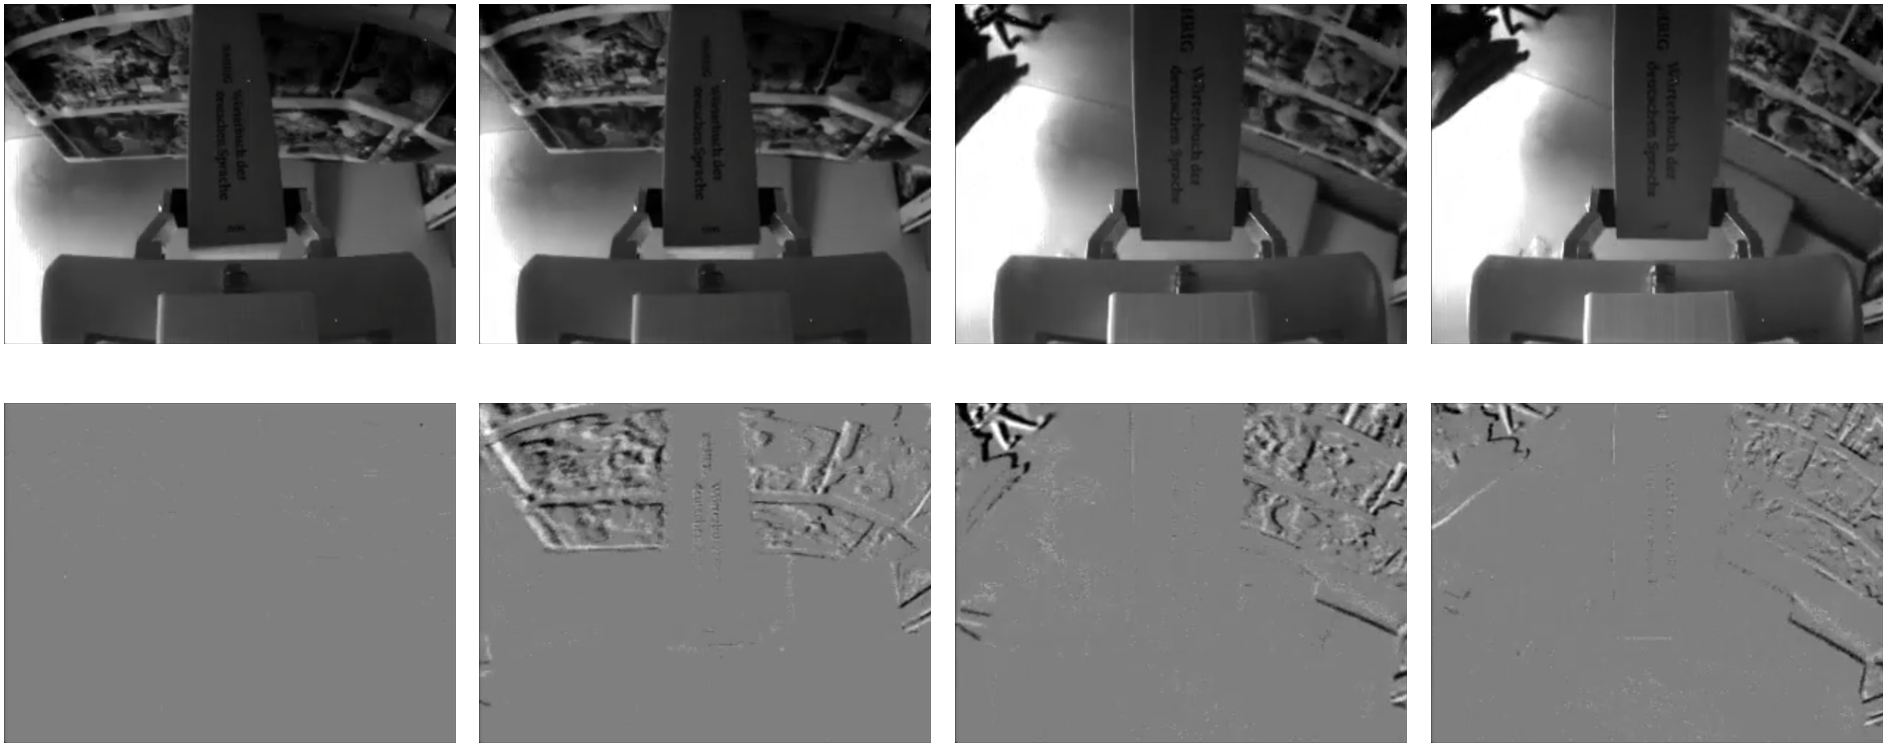
\includegraphics[width=\textwidth]{resources/images/set1_case7}
    \caption{Sequence of grayscale frames (first row) and event images (second row) during a significant slip, while executing a pick-and-place motion with book no. 1 and a highly textured table.}\label{fig:set1_case7}
\end{figure}

It is worth mentioning that all these experiments have been repeated 4-6 times in order to check the repeatability during the analysis of the slip detection.

\section{Set 2}

While analyzing Set 1, we realized that including the camera angular velocity would be informative to compute the motion flow in the scene and recording a sequence without grasping any object would enable us to compare against a sequence with an object and identify where the object located in the scene. These are the reasons behind recording a new set of data.\\

Moreover, in Set 1, the recorded data were mostly slip cases, so for this new set a balanced amount of slip and non-slip sequences has been recorded (3-5 times for each scenario).\\

In ~\Cref{fig:set2_empty} the usual trajectory is executed without grasping any object. Then, as shown in ~\Cref{fig:set2_case1}, a book is picked and no slip occurs during the whole sequence, which is accomplished by grasping the book approximately from its center and using a higher gripping force. In contrast, in ~\Cref{fig:set2_case2}, by grasping from the edge and using a lower force, a slip can be observed. Moreover, grasping from the other end of the book, there is a slip in the opposite direction, as depicted in ~\Cref{fig:set2_case3}.\\

Similarly, using another book, a non-slip case is observed in ~\Cref{fig:set2_case4} and a slip case is represented in ~\Cref{fig:set2_case5}.

\begin{figure}[H]
    \centering
    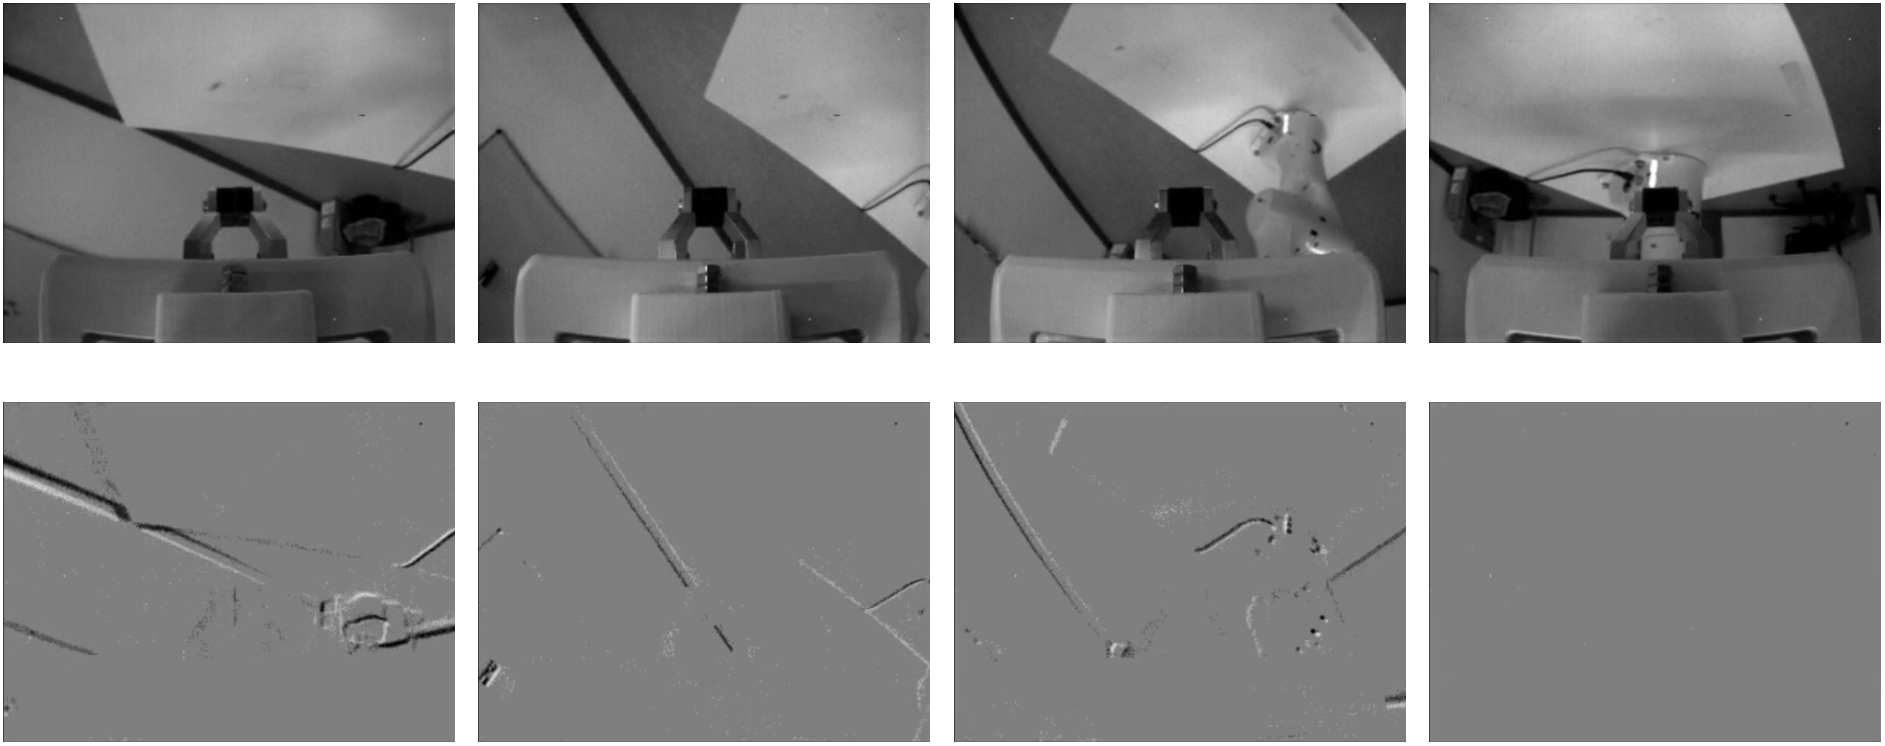
\includegraphics[width=\textwidth]{resources/images/set2_empty}
    \caption{Sequence of grayscale frames (first row) and event images (second row) while executing a pick-and-place motion without any object.}\label{fig:set2_empty}
\end{figure}

\begin{figure}[H]
    \centering
    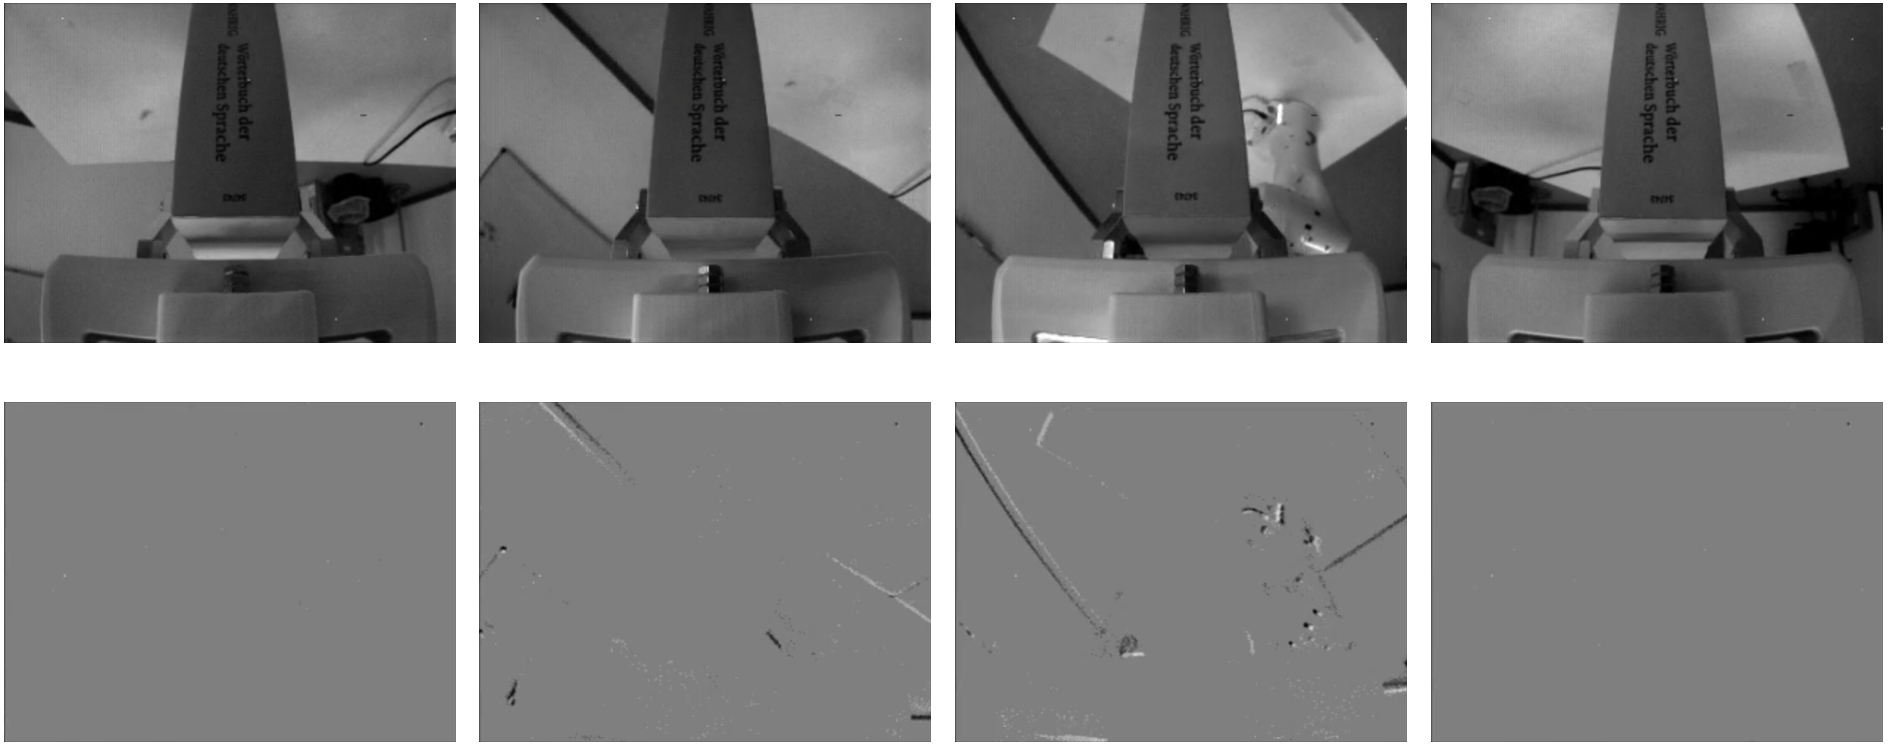
\includegraphics[width=\textwidth]{resources/images/set2_case1}
    \caption{Sequence of grayscale frames (first row) and event images (second row) during no slip, while executing a pick-and-place motion with book no. 1.}\label{fig:set2_case1}
\end{figure}

\begin{figure}[H]
    \centering
    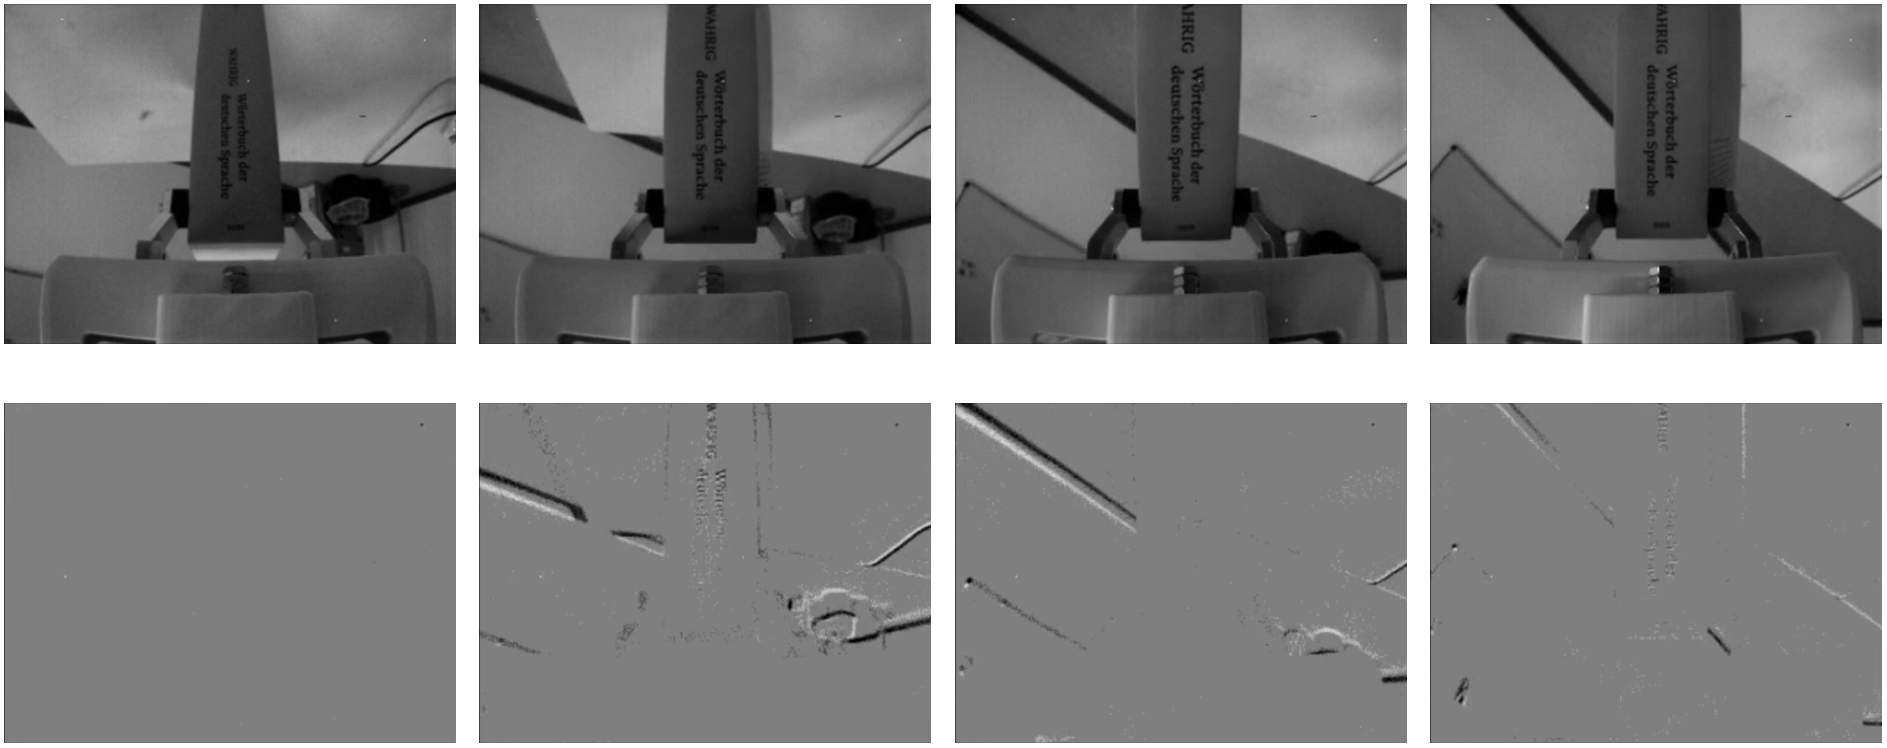
\includegraphics[width=\textwidth]{resources/images/set2_case2}
    \caption{Sequence of grayscale frames (first row) and event images (second row) during a significant slip, while executing a pick-and-place motion with book no. 1.}\label{fig:set2_case2}
\end{figure}

\begin{figure}[H]
    \centering
    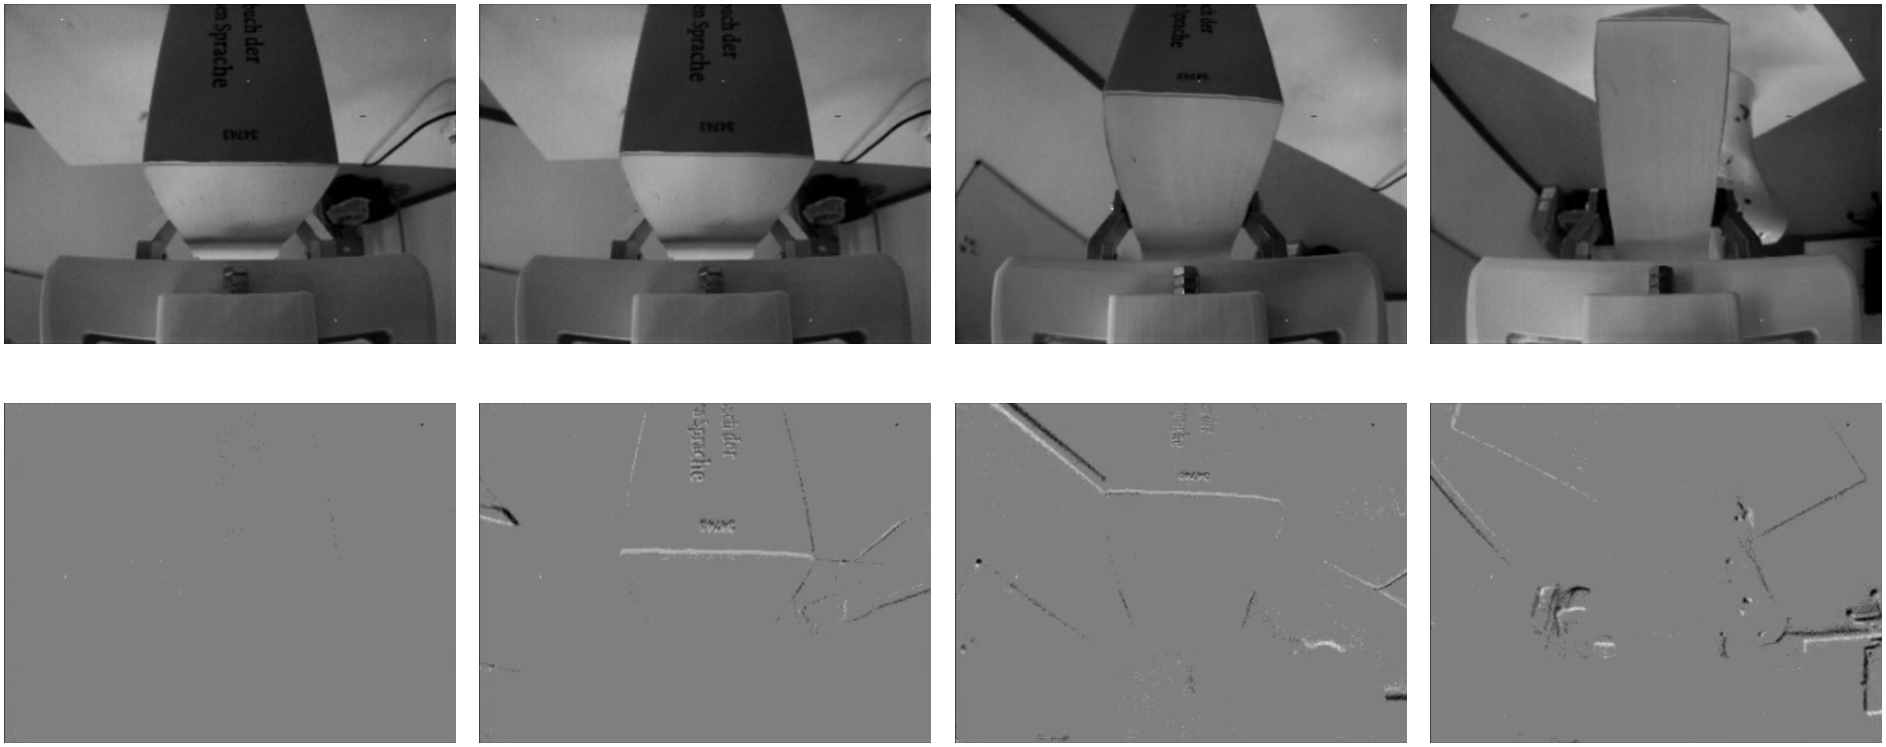
\includegraphics[width=\textwidth]{resources/images/set2_case3}
    \caption{Sequence of grayscale frames (first row) and event images (second row) during a significant slip, while executing a pick-and-place motion with book no. 1.}\label{fig:set2_case3}
\end{figure}

\begin{figure}[H]
    \centering
    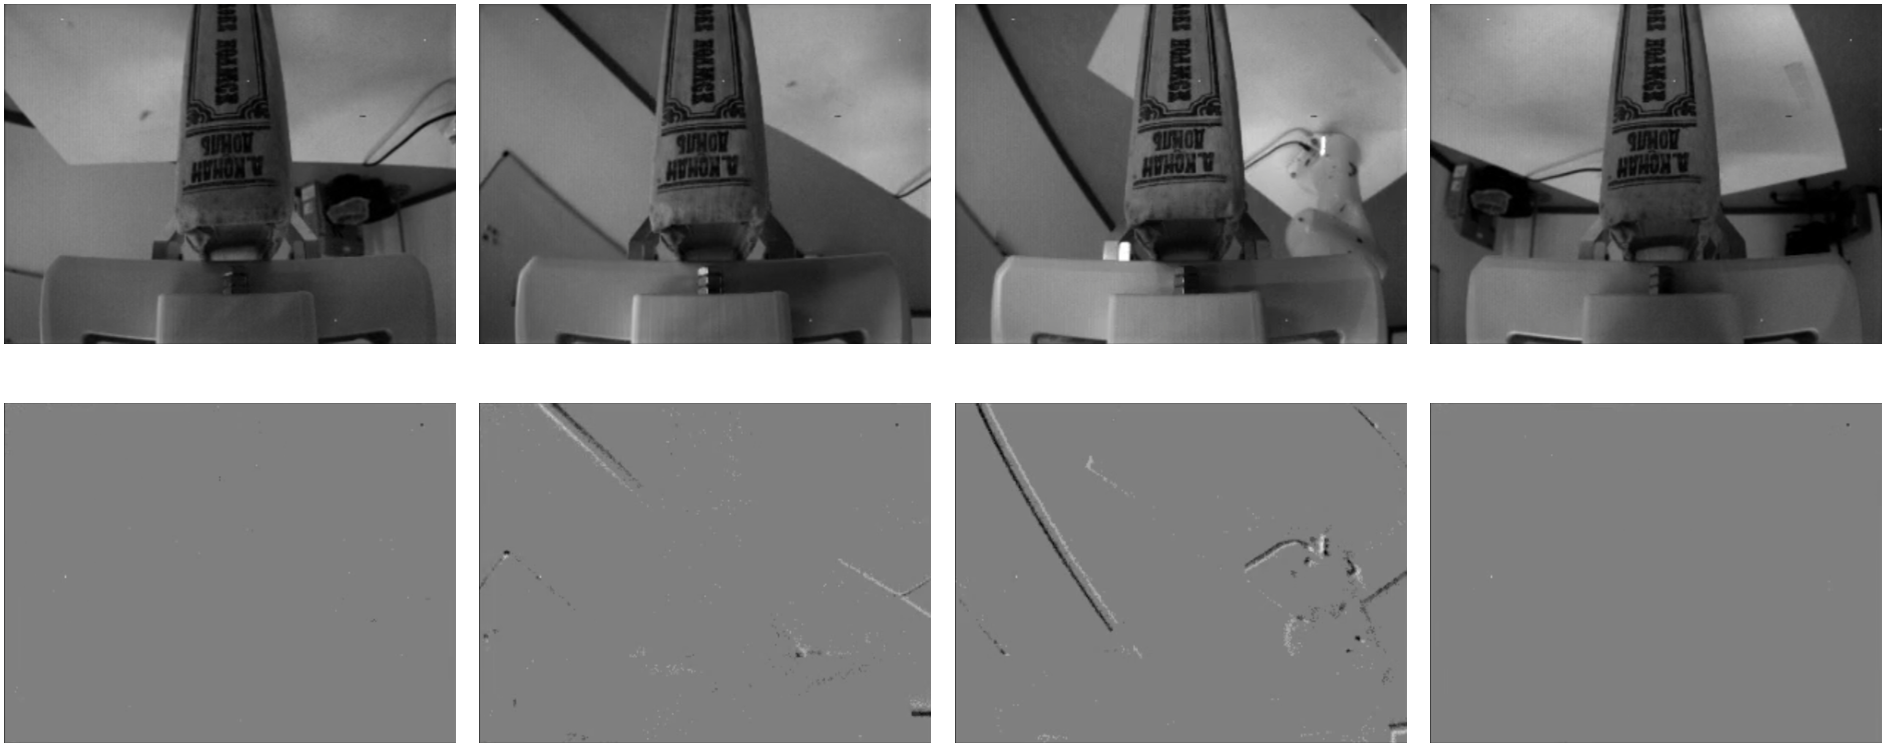
\includegraphics[width=\textwidth]{resources/images/set2_case4}
    \caption{Sequence of grayscale frames (first row) and event images (second row) during no slip, while executing a pick-and-place motion with book no. 2.}\label{fig:set2_case4}
\end{figure}

\begin{figure}[H]
    \centering
    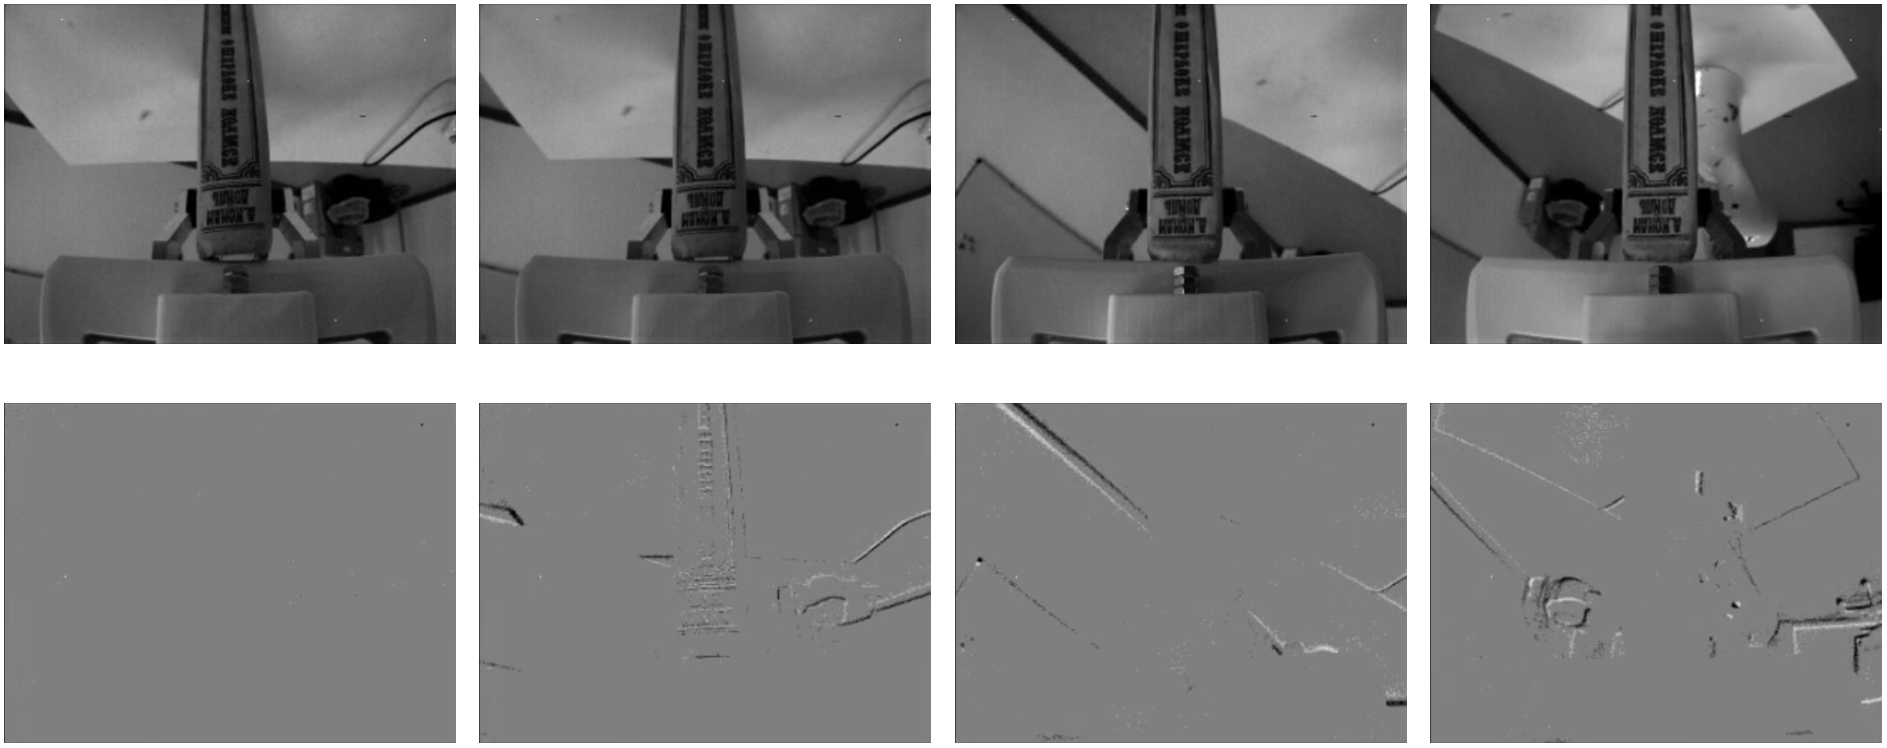
\includegraphics[width=\textwidth]{resources/images/set2_case5}
    \caption{Sequence of grayscale frames (first row) and event images (second row) during a significant slip, while executing a pick-and-place motion with book no. 2.}\label{fig:set2_case5}
\end{figure}

\section{Set 3}

The previous sets of data present one issue: the labeling of the time when a slip occurs has to be done manually. To solve this issue, ground-truth data should be saved in parallel with the rest of the data gathered until now. Concretely, we use a motion capture system, called OptiTrack, which consists of several cameras that track certain markers. These markers can be placed in rigid bodies and, once they are defined as so in \textit{Motive} (a optical motion capture software), the objects can be tracked with positional accuracies of $\pm 0.2$ mm and rotational accuracies of $\pm 0.1$º. In ~\Cref{fig:optitrack}, the new experiment setup is shown, with the OptiTrack cameras located at the top, and the object with markers shown in the bottom right part. 

\begin{figure}[H]
    \centering
    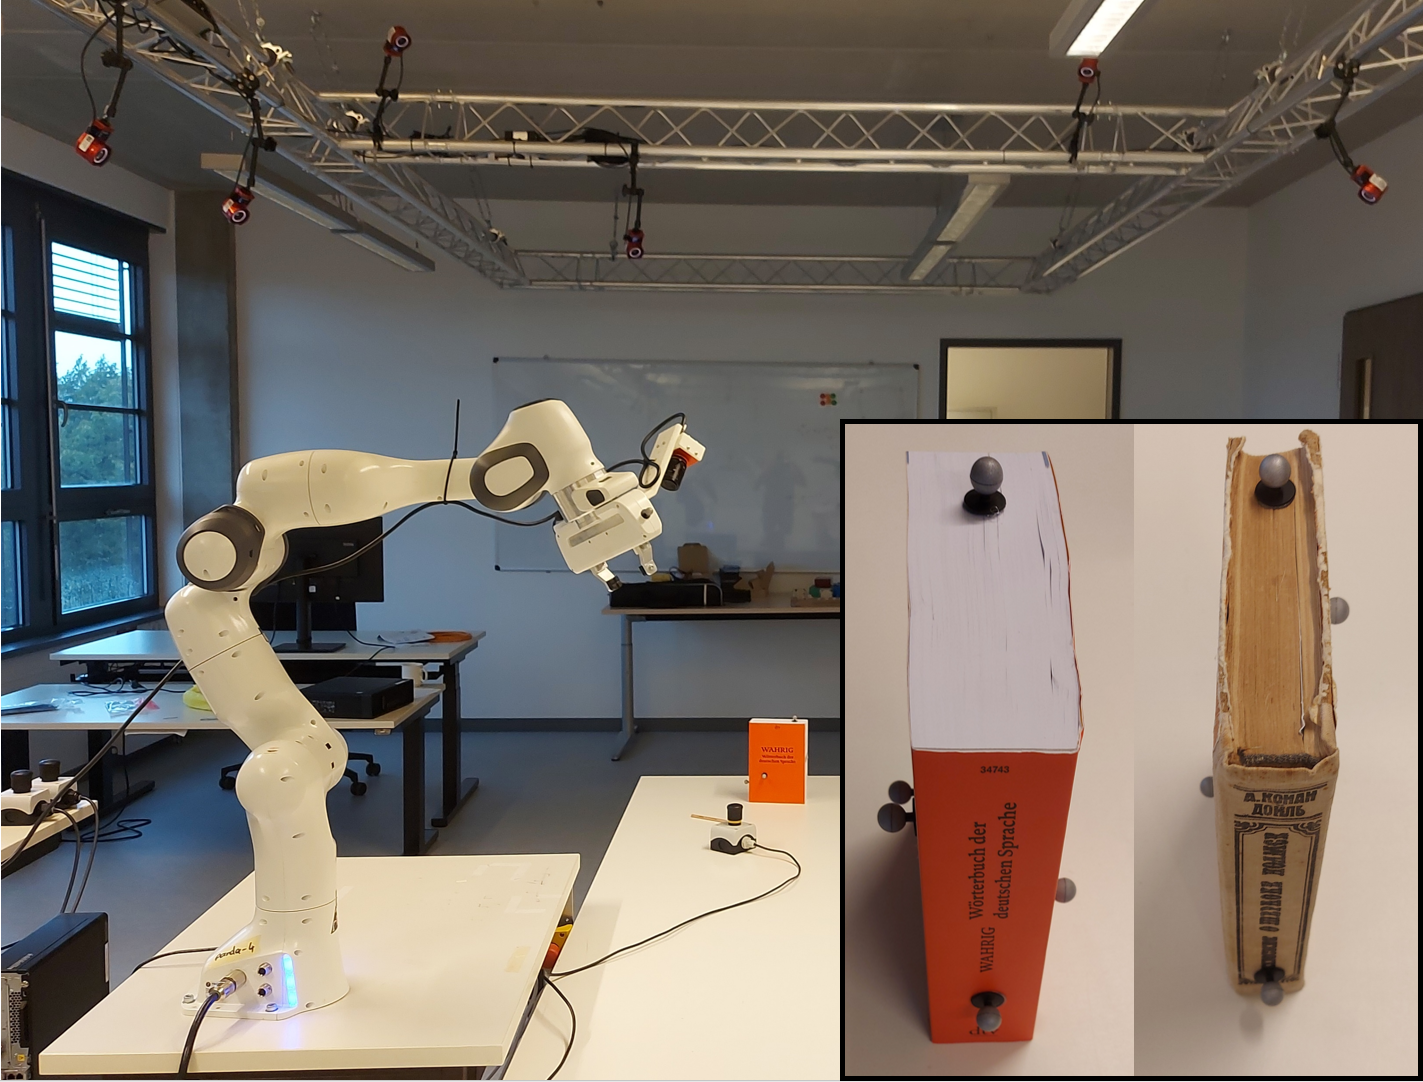
\includegraphics[width=0.9\textwidth]{resources/images/optitrack_setup}
    \caption{Experiment Setup including OptiTrack cameras and objects with markers.}\label{fig:optitrack}
\end{figure}

The recorded data is quite similar to Set 2, just changing the background, having more elements in this new set, and including the information received from the OptiTrack. Concretely, the pose of the gripper and the grasped object are tracked. With that, we can analyze the relative pose of the object with respect to the gripper and detect if slip occurred.\\

Again sequences with and without slip have been recorded for two books, with 5 repetitions for each scenario.\\

For the first book, as shown in ~\Cref{fig:set3_case1}, only a slight rotation is produced towards the end, whereas in \Cref{fig:set3_case2}, there is a slip in the beginning, then it stops and slips again in the opposite direction.\\

In the case of the second book, a similar behavior is observed, with nearly no slip in \Cref{fig:set3_case3} and slip in \Cref{fig:set3_case4}.

\begin{figure}[H]
    \centering
    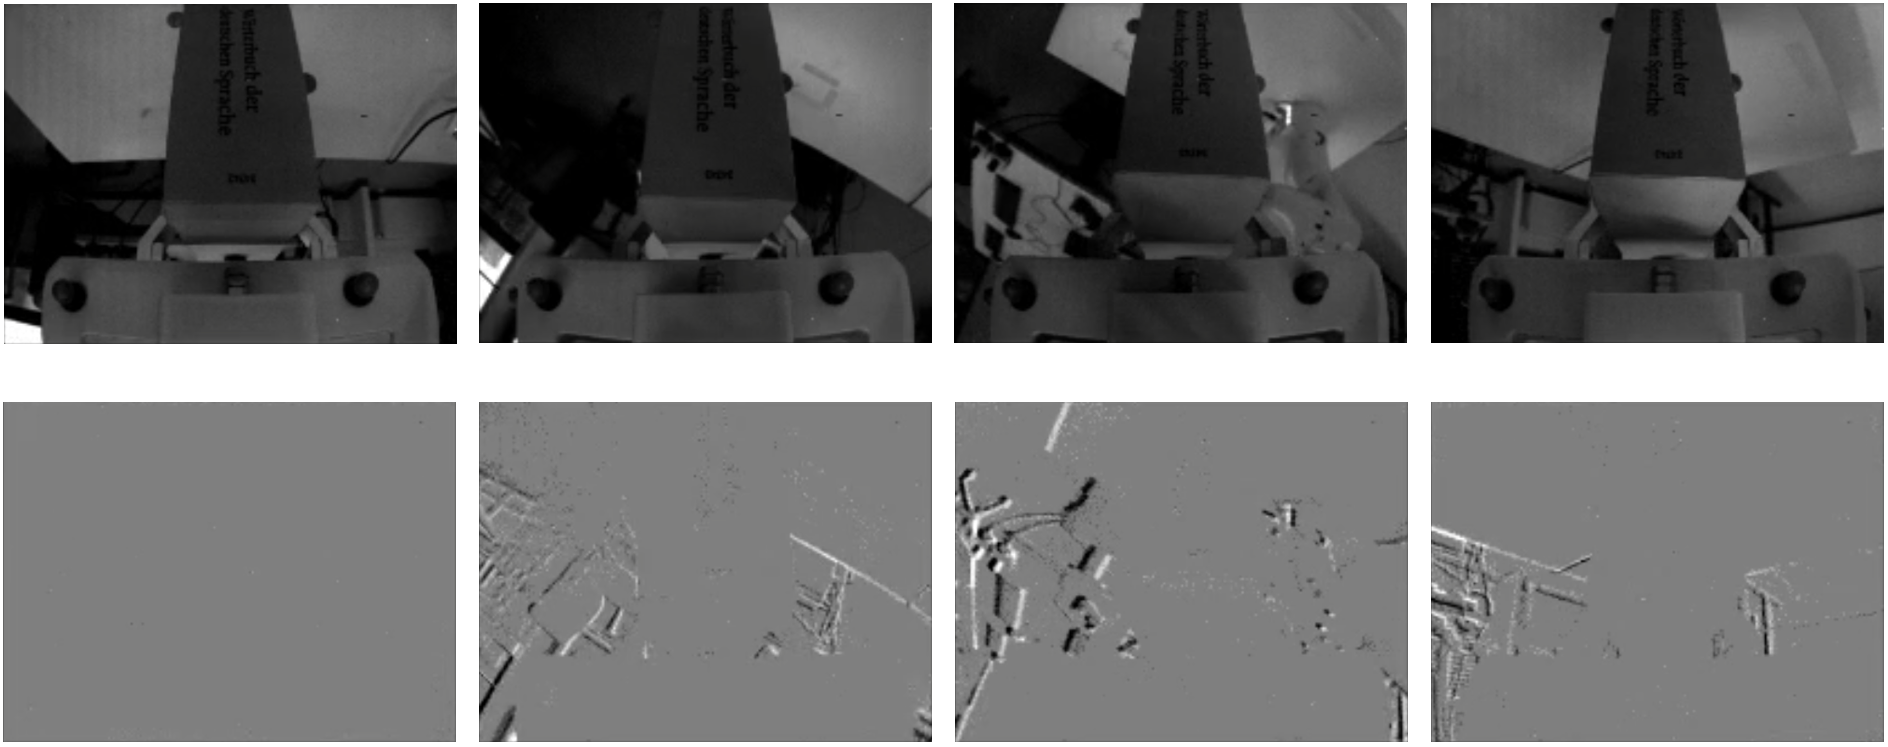
\includegraphics[width=\textwidth]{resources/images/set3_case1}
    \caption{Sequence of grayscale frames (first row) and event images (second row) during no slip, while executing a pick-and-place motion with book no. 1.}\label{fig:set3_case1}
\end{figure}

\begin{figure}[H]
    \centering
    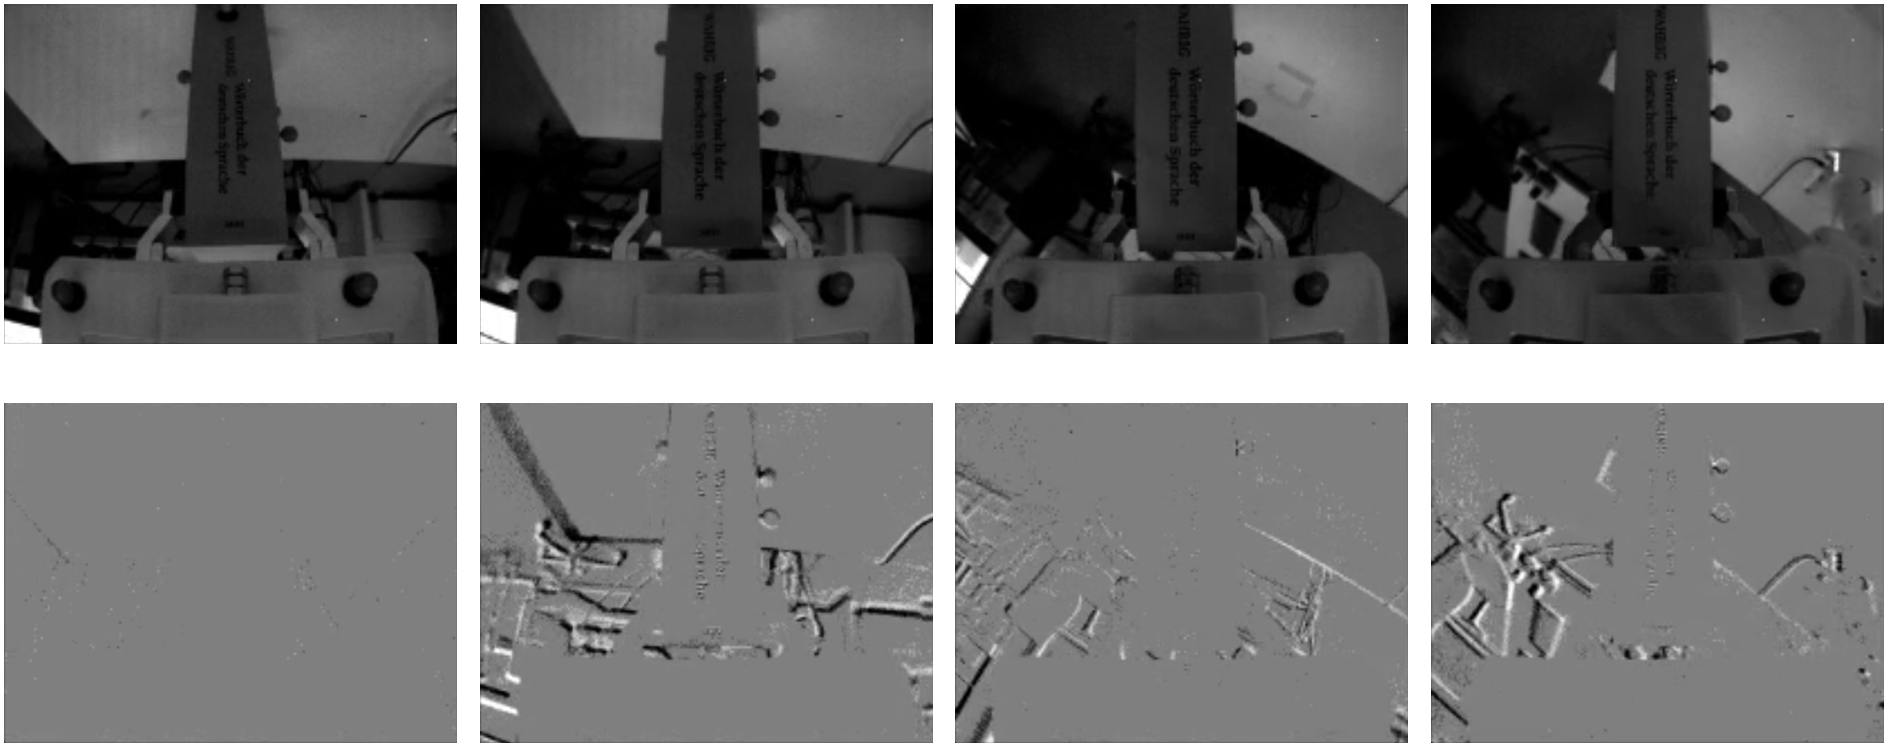
\includegraphics[width=\textwidth]{resources/images/set3_case2}
    \caption{Sequence of grayscale frames (first row) and event images (second row) during a significant slip, while executing a pick-and-place motion with book no. 1.}\label{fig:set3_case2}
\end{figure}

\begin{figure}[H]
    \centering
    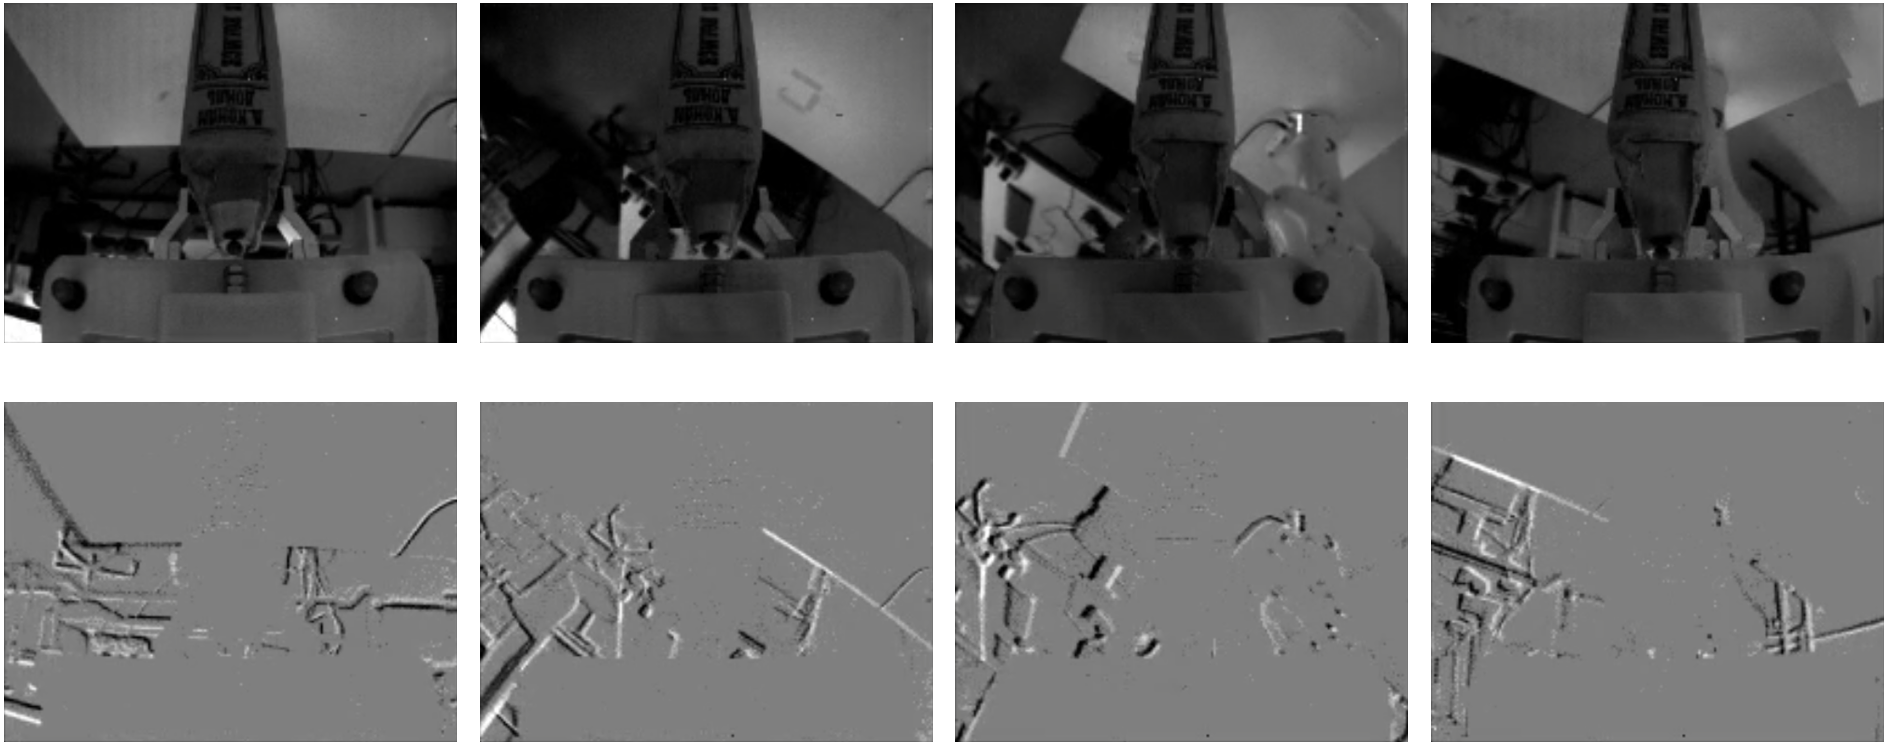
\includegraphics[width=\textwidth]{resources/images/set3_case3}
    \caption{Sequence of grayscale frames (first row) and event images (second row) during a significant slip, while executing a pick-and-place motion with book no. 2.}\label{fig:set3_case3}
\end{figure}

\begin{figure}[H]
    \centering
    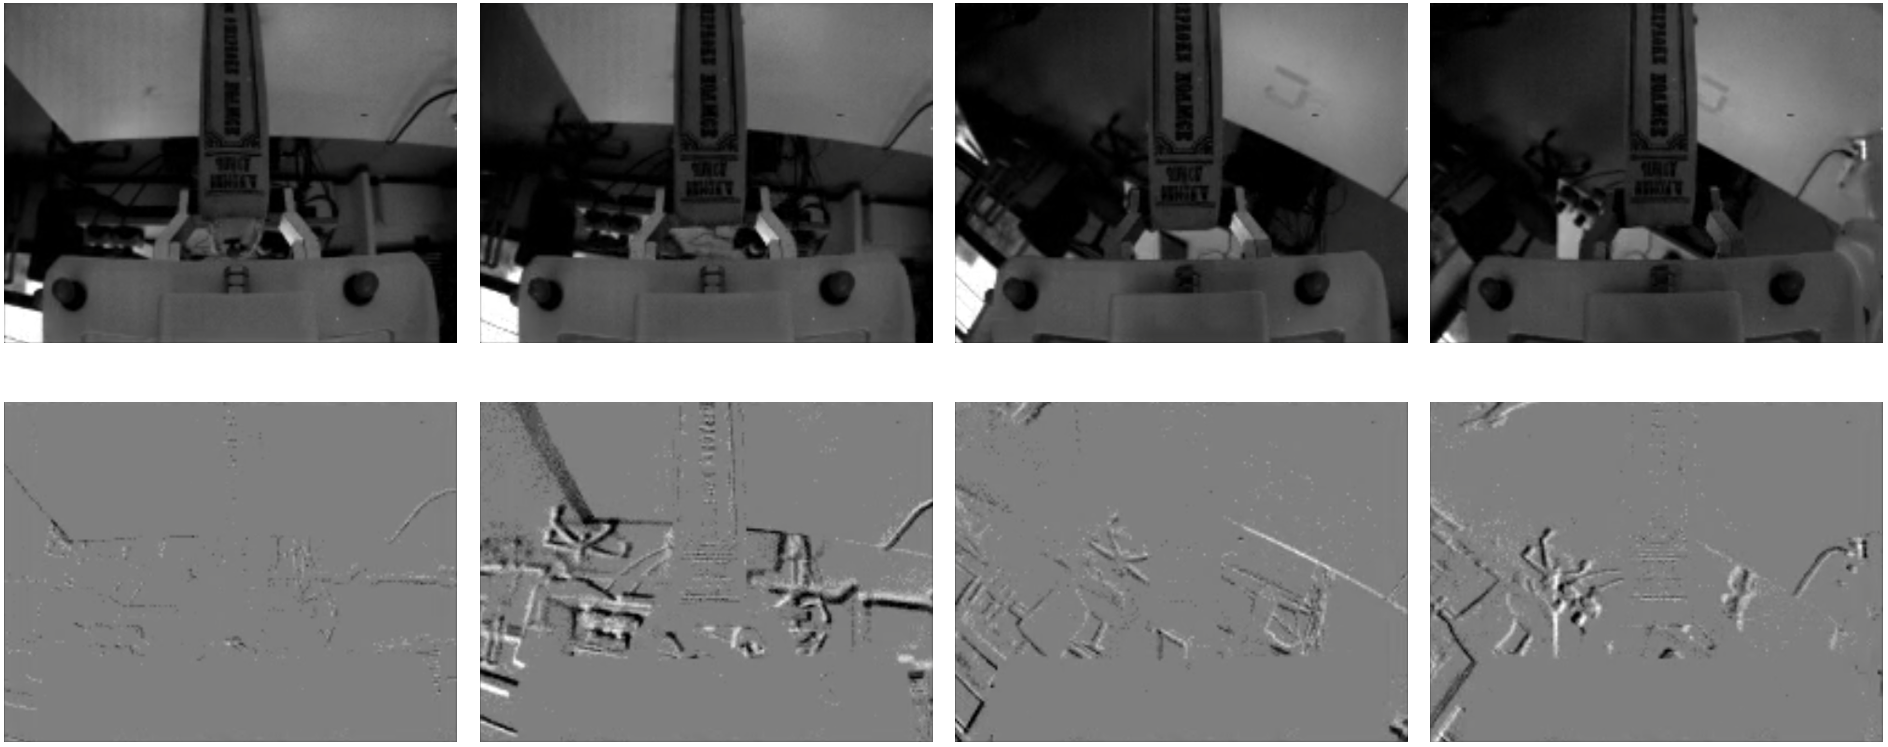
\includegraphics[width=\textwidth]{resources/images/set3_case4}
    \caption{Sequence of grayscale frames (first row) and event images (second row) during no slip, while executing a pick-and-place motion with book no. 2.}\label{fig:set3_case4}
\end{figure}

\section{Conclusion}

In this chapter, all the recorded data is described, the gathering of which was done iteratively, after analyzing the data and determining the new needs after each step. Therefore, these sets of data are meant to help to explore different methods to detect slip and do not make up a final dataset, which should include many more sequences and objects.\\

The next chapter includes the description of the different methods tested to determine slip cases and the discussion of their results.



    \cleardoublepage
\chapter{Slip detection methods}\label{sec:methods}

\section{Event rate analysis}

\subsection{Introduction}

We know that, if there is no slip, the object moves along with the gripper and camera, therefore, there will not be any moving edges in the event images. On the contrary, if slip occurs, moving edges will appear depending on the texture of the grasped object.\\

Thus, it might be interesting to analyze the event rate coming from the object, which may increase significantly depending if there is slip or not. As the object may change its shape significantly from the camera's view during the slip, it is challenging to focus only on the events generated by the object. Also, events may be produced by changes in illumination, for that, it may also be informative and more robust to analyze the ratio between the events produced by the object and the total number of events.

\subsection{Results with Gelsight dataset}

To verify the aforementioned idea, first, the described event rate was analyzed with an existing dataset ~\cite{gelsight2018}, which is suitable for an initial analysis as the sequences are formed just by the initial 1 second of the lifting phase with a uniform background, including daily use objects. Nevertheless, the data contains only RGB frames coming from a standard webcam. Therefore, these sequences of images should be converted into events, which has been done using \textit{v2e} ~\cite{v2e}. This algorithm gets the events from a RGB video, first converting the frames to grayscale and then slowing down the video (by interpolating the frames) in order to compute the events with a lower latency.\\

For object 1 of the dataset and using a gripper width of 66.6 mm, the grasp is perfect and no slip occurs, as observed in ~\Cref{fig:gelsight_case1}. This case is labeled as "ok" in the dataset, meaning that the grasp occurred successfully. In addition, as the background is quite uniform, nearly no events are generated from it and only some appear from the borders of the table.

\begin{figure}[H]
    \centering
    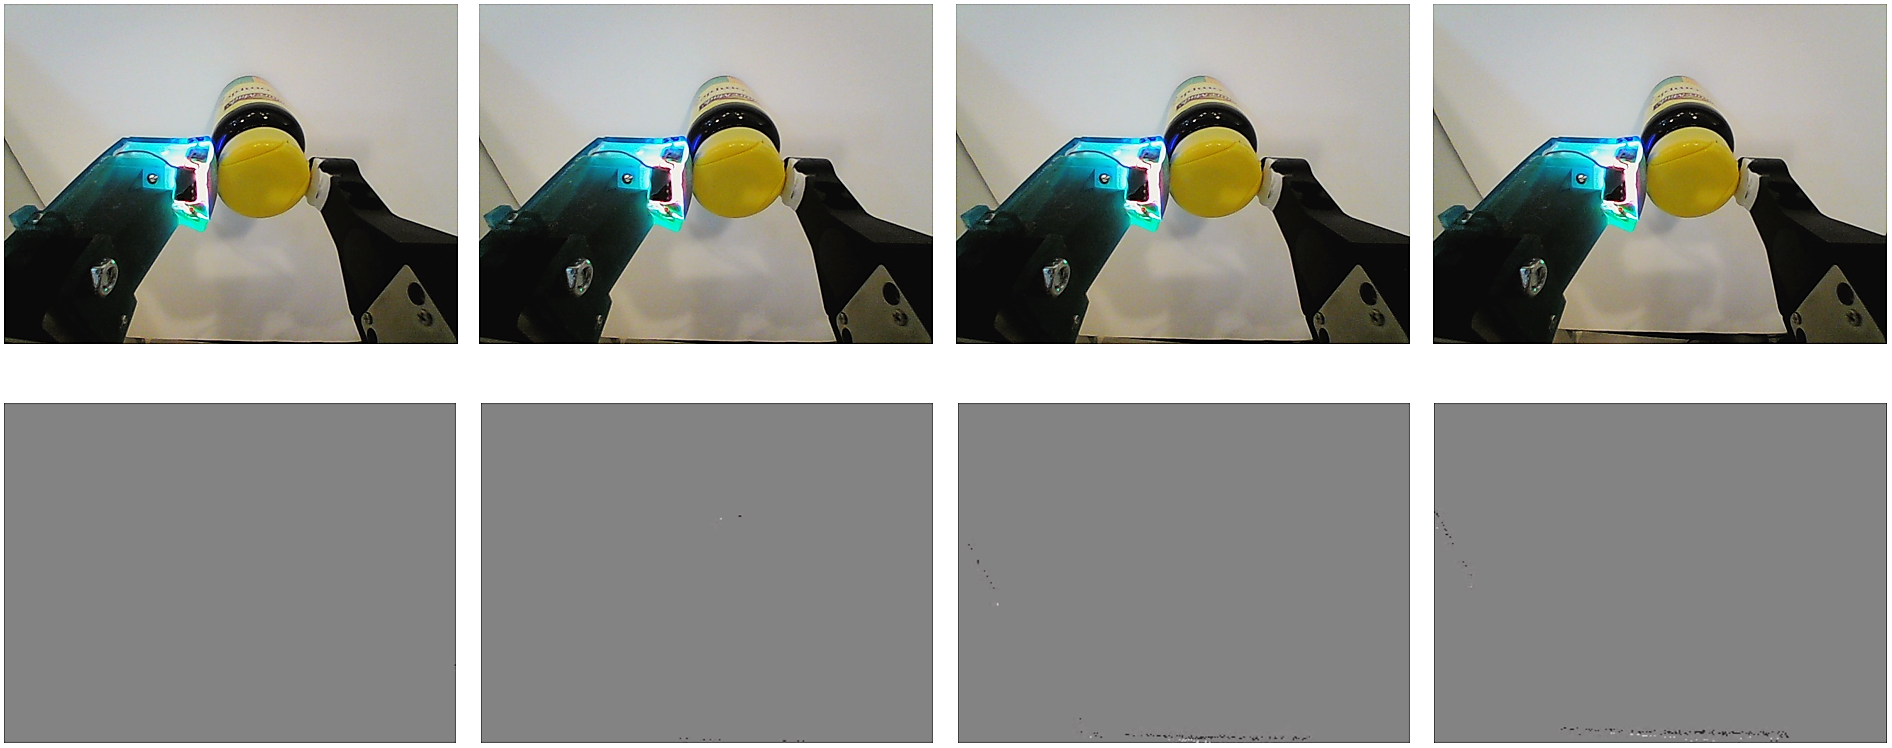
\includegraphics[width=\textwidth]{resources/images/gelsight_case1}
    \caption{Sequence of RGB frames (first row) and event images (second row) with object 1 from the dataset in ~\cite{gelsight2018} and a gripper width of 66.6 mm.}\label{fig:gelsight_case1}
\end{figure}

Opening a bit more the gripper, concretely with a width of 67.2 mm, the grasp is still labeled as "ok", but some events appear in the middle of the lift, as represented in ~\Cref{fig:gelsight_case2}. Nevertheless, this minor slip does not affect the grasp and the object is lifted successfully.

\begin{figure}[H]
    \centering
    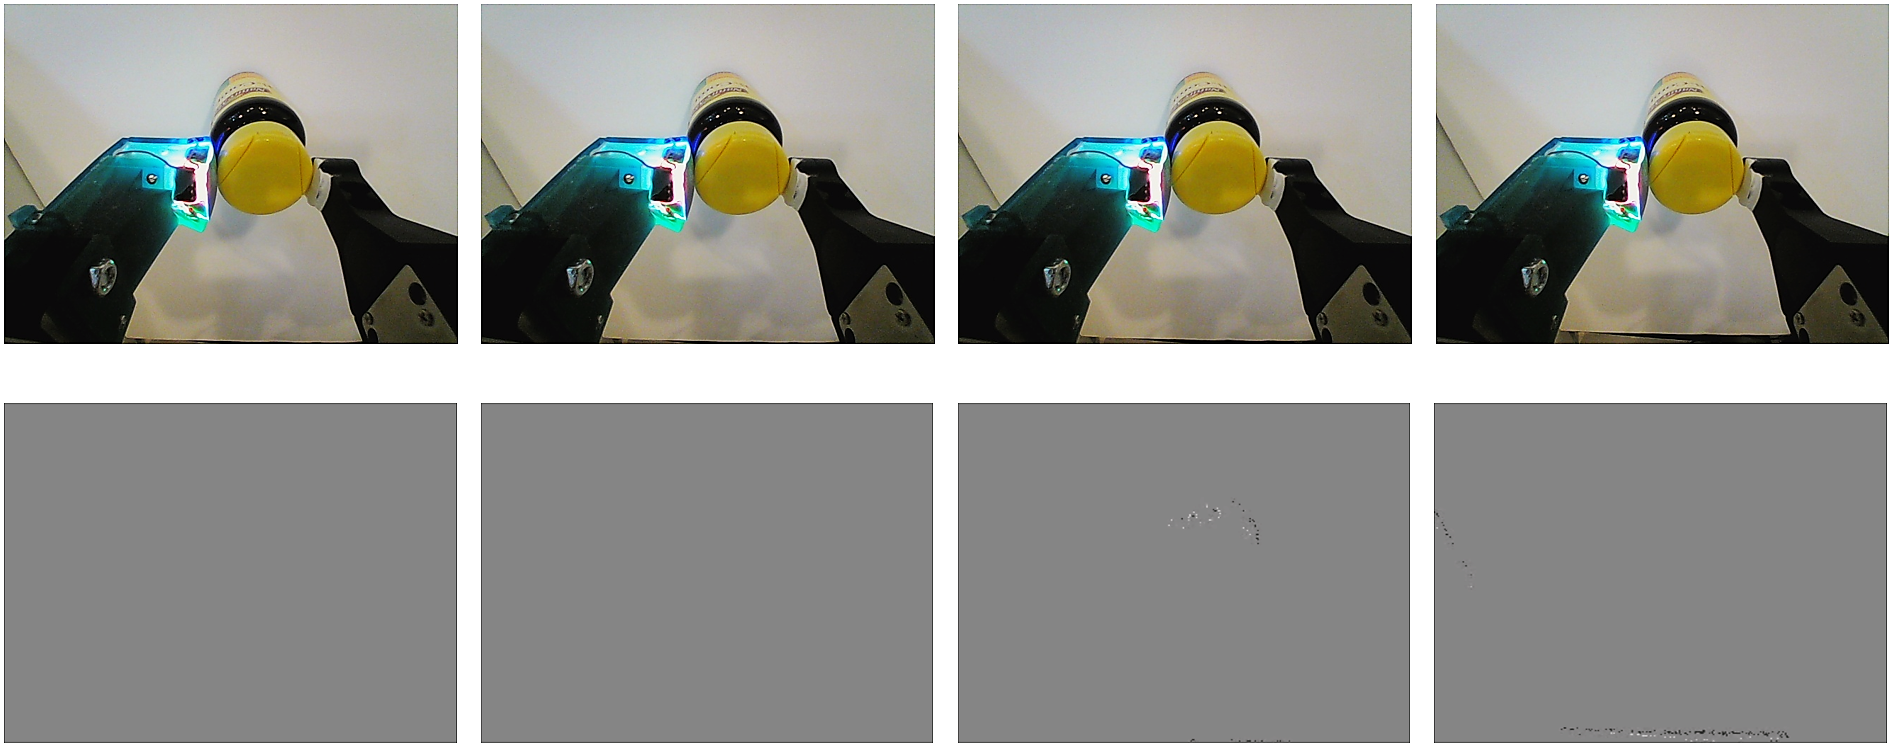
\includegraphics[width=\textwidth]{resources/images/gelsight_case2}
    \caption{Sequence of RGB frames (first row) and event images (second row) with object 1 from the dataset in ~\cite{gelsight2018} and a gripper width of 67.2 mm.}\label{fig:gelsight_case2}
\end{figure}

With a gripper width of 67.3 mm, the first sample labeled as "fail" can be found. As depicted in ~\Cref{fig:gelsight_case3}, a minor slip occurs in the beginning of the lift, then it stops slipping and just in the end the object starts falling.\\

\begin{figure}[h]
    \centering
    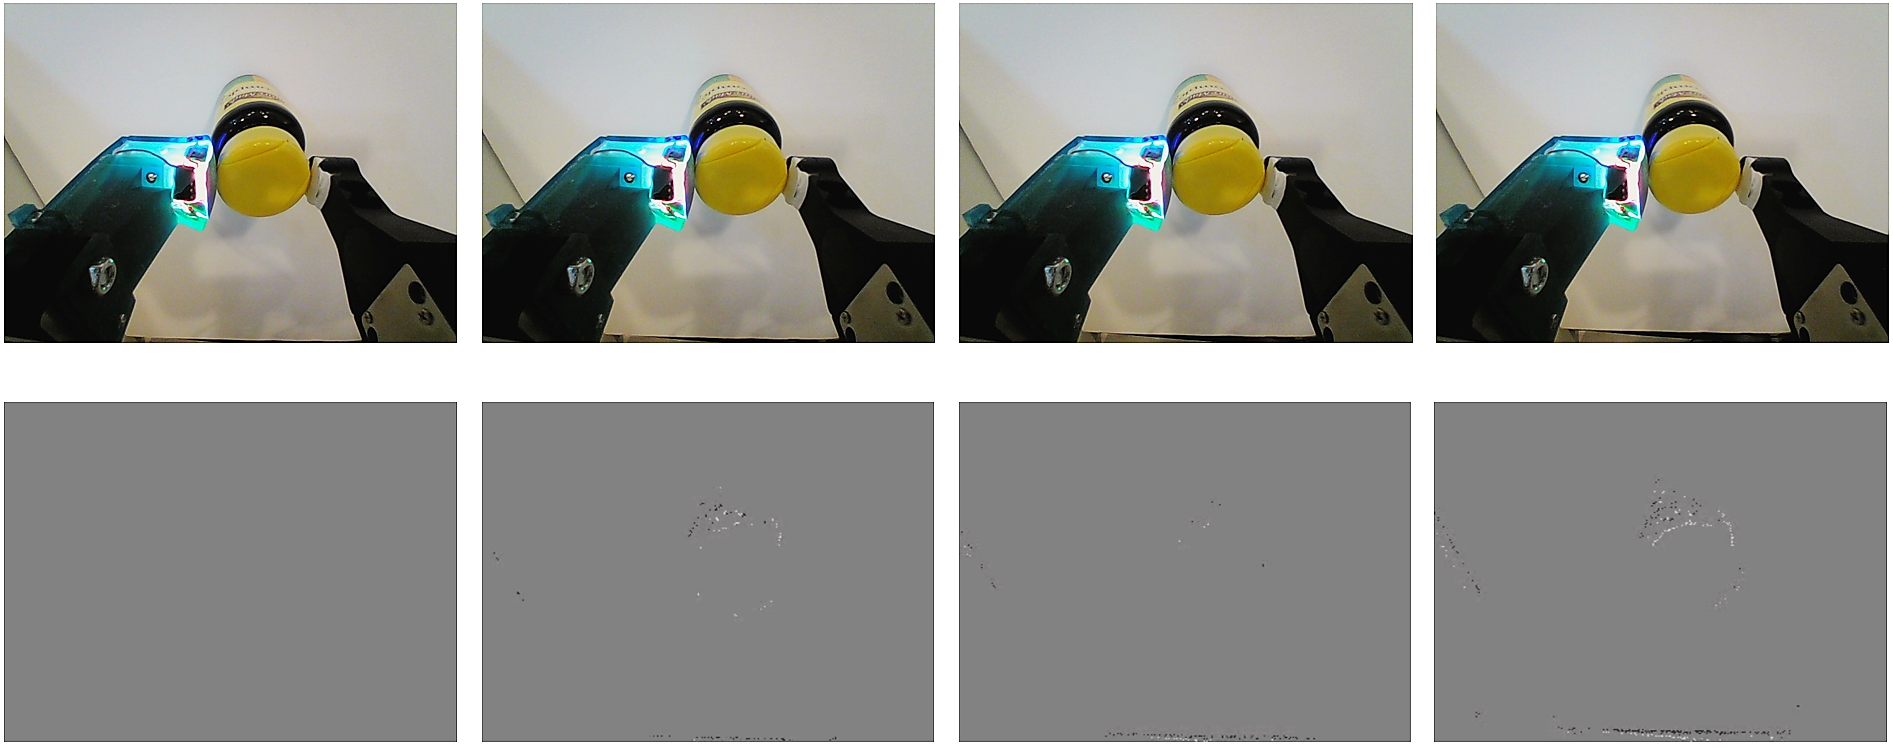
\includegraphics[width=\textwidth]{resources/images/gelsight_case3}
    \caption{Sequence of RGB frames (first row) and event images (second row) with object 1 from the dataset in ~\cite{gelsight2018} and a gripper width of 67.3 mm.}\label{fig:gelsight_case3}
\end{figure}

Finally, opening the gripper until 67.5 mm, produces a clear grasping failure, not even lifting the object, as shown in ~\Cref{fig:gelsight_case4}, where events are coming from the object continuously, while the gripper moves away from it without grasping it.\\

\begin{figure}[h]
    \centering
    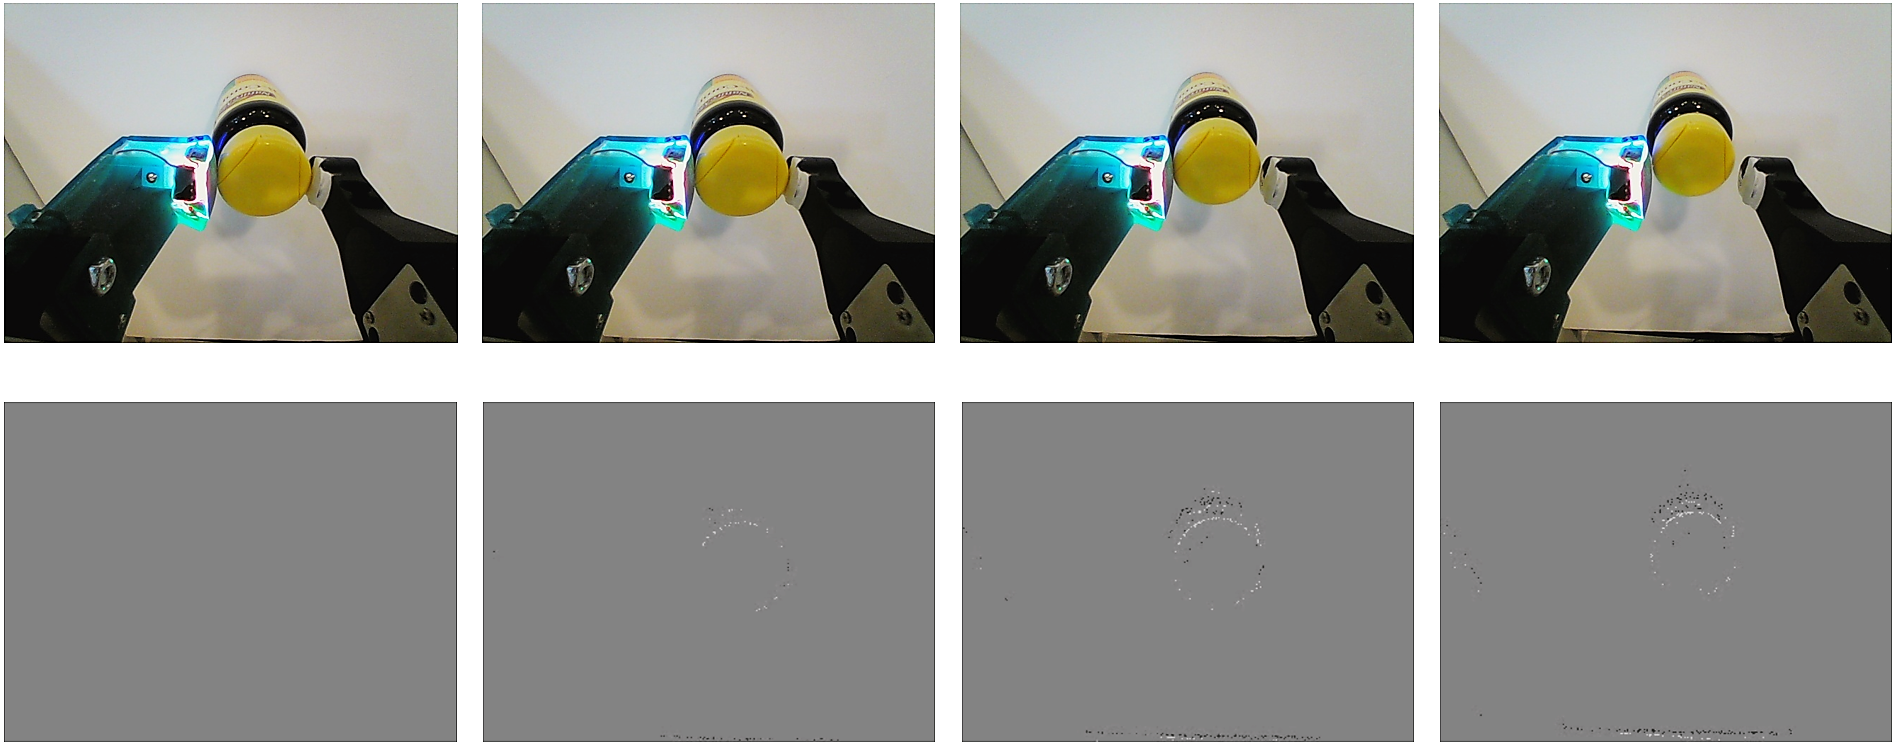
\includegraphics[width=\textwidth]{resources/images/gelsight_case4}
    \caption{Sequence of RGB frames (first row) and event images (second row) with object 1 from the dataset in ~\cite{gelsight2018} and a gripper width of 67.5 mm.}\label{fig:gelsight_case4}
\end{figure}

With these 4 samples, the event rate in the whole image can be computed as a first analysis, instead of focusing only in the object, as the background is quite uniform, thus not many events will be generated by it. Also, the background is constant in all the samples, so the events generated from it will also be the same for each sample, being the only difference the events associated to the object movement.

In ~\Cref{fig:gelsight_evr}, the evolution of the event rate in the whole image for the 4 detailed examples is shown. This event rate has been computed counting the events during consecutive time windows of 10 ms, value selected in order to have the lowest latency possible without having a really noisy signal. For the two cases labeled as "ok", similar evolutions can be observed, increasing the event rate towards the end, due to the background events. With a gripper width of 67.3 mm, there is a slip in the beginning of the lift and the event rate is higher than the previous two examples between 0.5 and 0.6 seconds due to it. Additionally, towards the end, the object starts falling and many events appear in the scene, which is reflected by the high peak in the end of the sequence. Finally, for the last experiment, the event rate is clearly higher than the other samples during the whole sequence due to the grasp failure.\\

\begin{figure}[h]
    \centering
    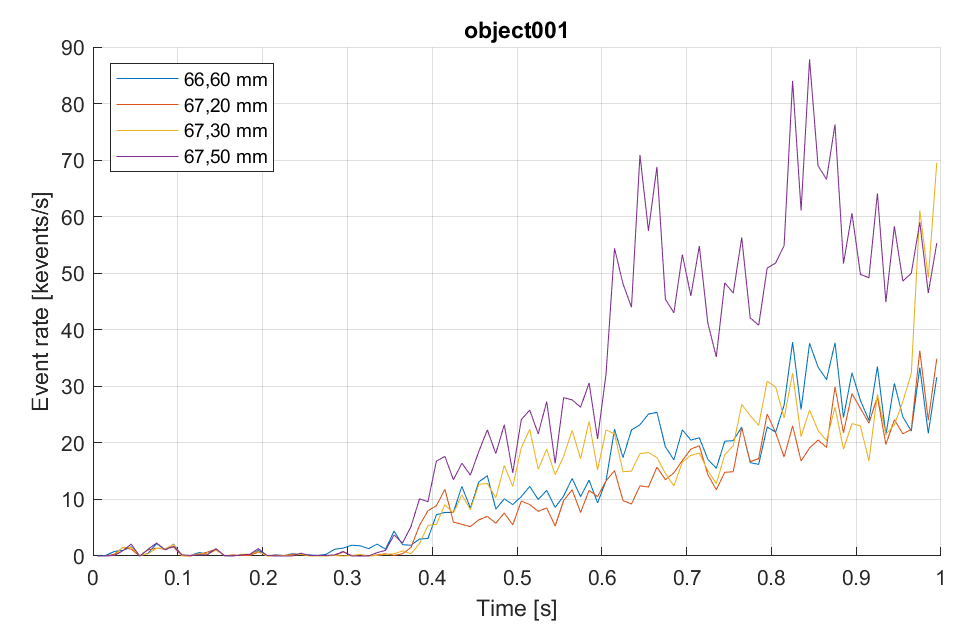
\includegraphics[width=\textwidth]{resources/images/gelsight_evr}
    \caption{Comparison of the event rate evolution in the whole image for 4 samples of object 1 from the dataset in ~\cite{gelsight2018}.}\label{fig:gelsight_evr}
\end{figure}

Thanks to this analysis, the usefulness of the event rate for slip detection is proved. For instance, if this one dimensional signal surpasses a certain threshold (40 kevents/s in this example), a slip can be detected. However, it is true that in this case the background is uniform and constant during all the experiments, this is why only with the event rate in the whole image is enough to detect slip, which may not be the case in our sets of data.\\

As an example, only the first object of the dataset has been analyzed in detail here, but the drawn conclusions apply also to other objects and experiments.

\subsection{Results with Set 1 and fixed RoI}

In our dataset, the background is not uniform, therefore, in order to detect slip we need to focus on the events coming from the object. One naive approach is to manually annotate with a rectangle where the object is in the first frame (just when the gripper has closed in the picking phase), which is denoted as the Region of Interest (RoI), and keep it fixed during the whole sequence, assuming that the object will stay in that region during the whole motion. Of course, using a rectangle is the simplest option, but it may not fit properly the object, including some parts of the background in the RoI. Also, keeping it fixed means that during the sequence, if there is a slip, the object may fall out of the RoI or more background parts fall into it. In ~\Cref{fig:fix_roi} some examples of manually annotated RoIs are depicted.

\begin{figure}[h]
    \centering
    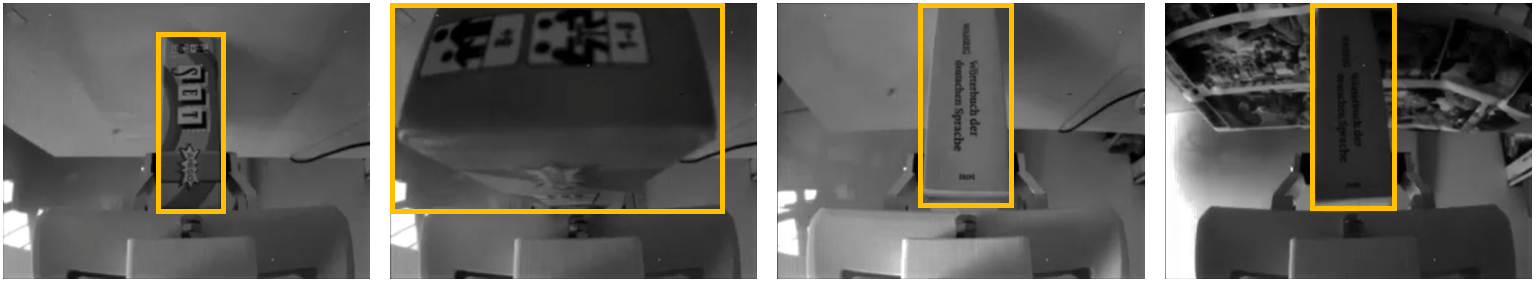
\includegraphics[width=\textwidth]{resources/images/fix_roi}
    \caption{Example initial frames of Set 1, with their respective fix RoI.}\label{fig:fix_roi}
\end{figure}

In ~\Cref{fig:fix_roi_set}, the evolution of the event rates for the RoI and the whole image have been represented, considering a time window of 10 ms, for the sequences like the ones shown in ~\Cref{fig:set1_case1} and ~\Cref{fig:set1_case2}. In addition, the ratio between these two signals is included, which is better suited to be thresholded, as it is bounded between 0 and 1. This signal can be interpreted as the relative amount of events of events inside the RoI compared to the whole image, which intuitively seems informative of slip cases. 

\begin{figure}[h]
    \centering
    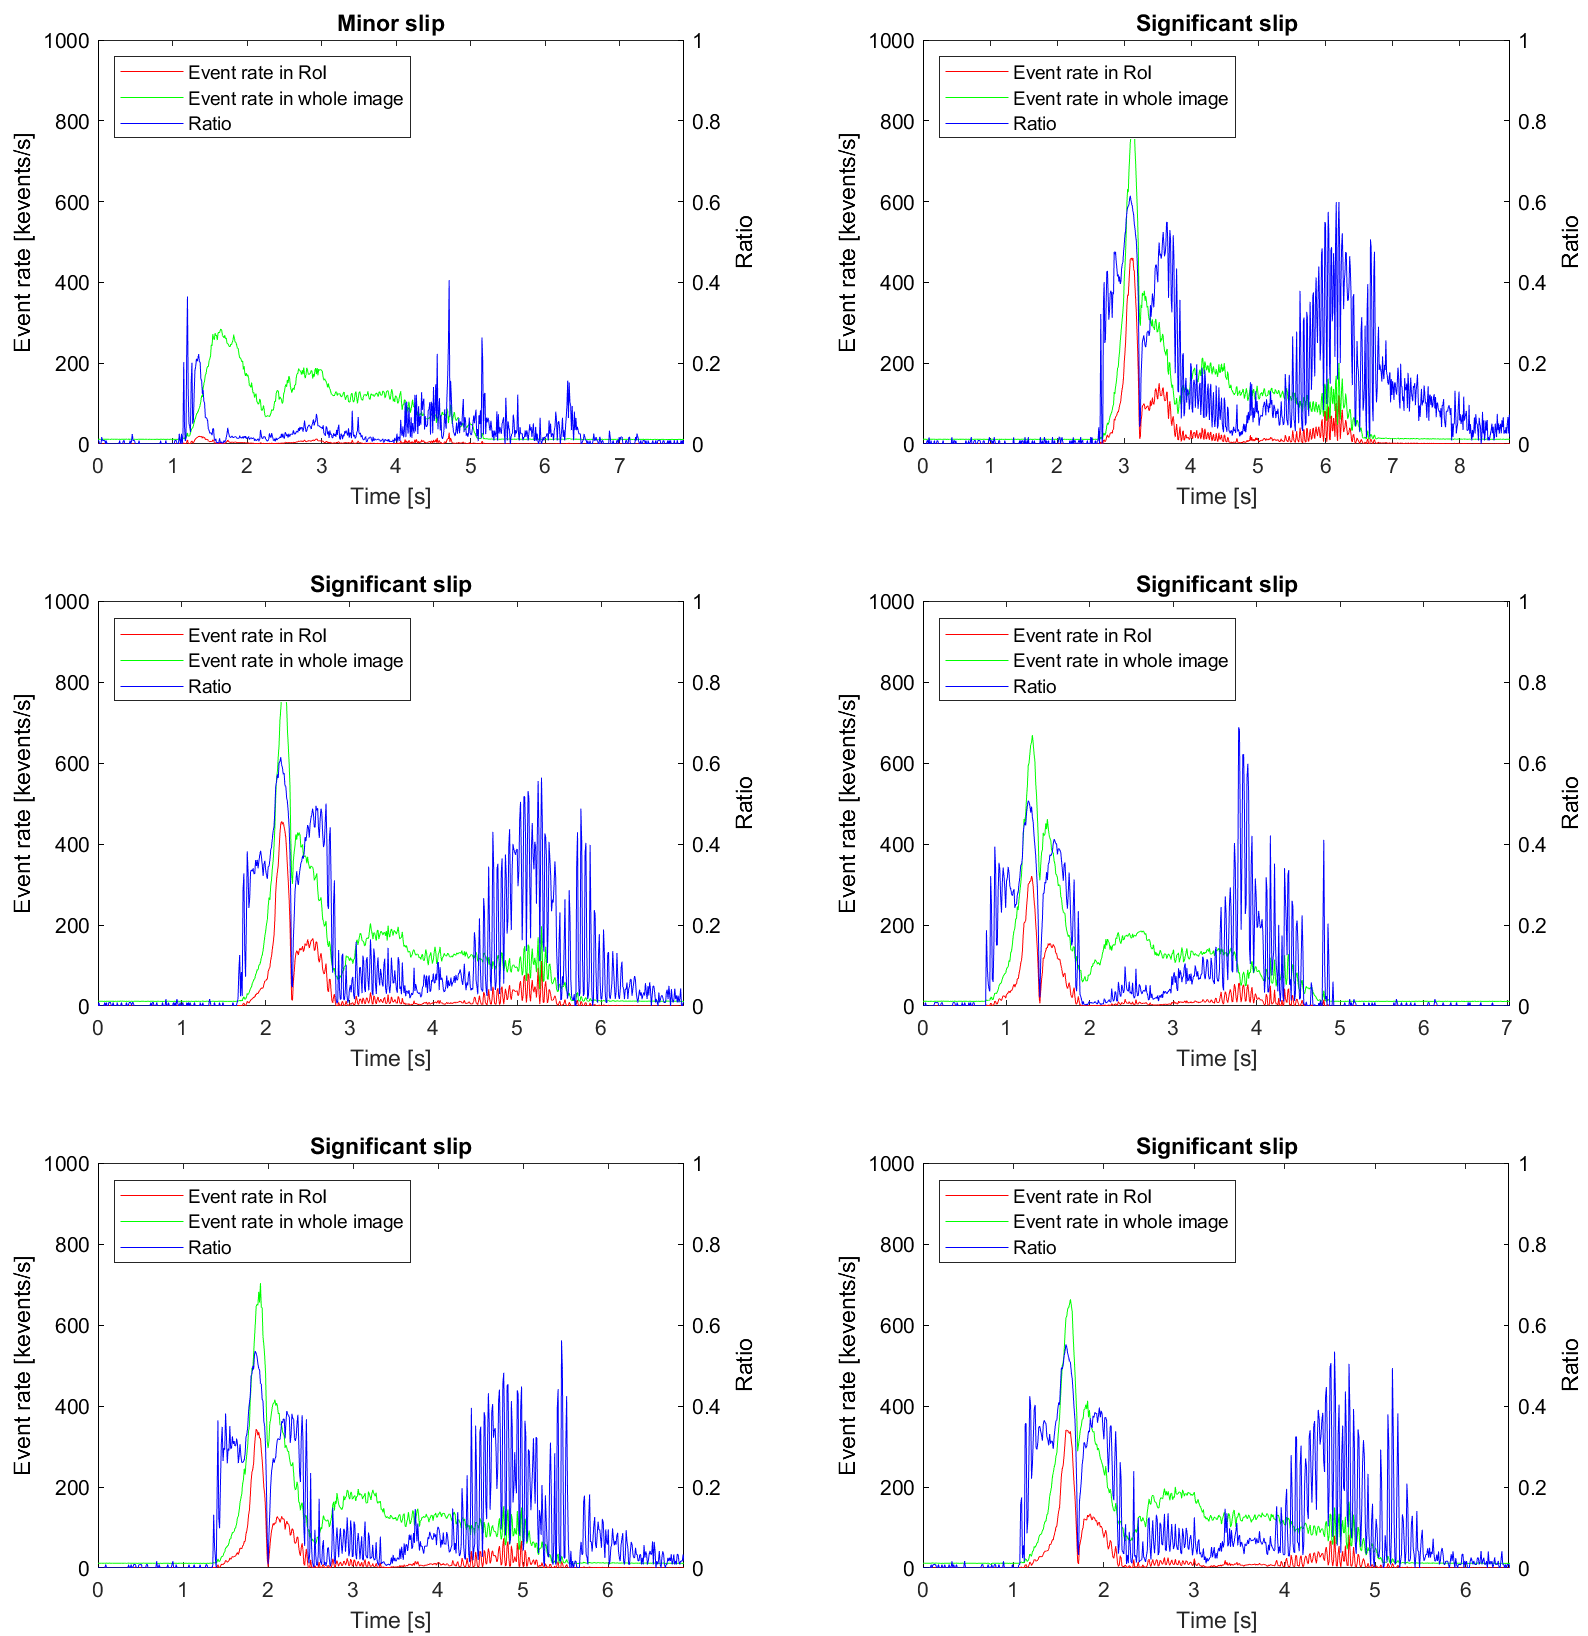
\includegraphics[width=\textwidth]{resources/images/fix_roi_set}
    \caption{Event rate and ratio signals during a pick-and-place motion with a box using a fixed RoI.}\label{fig:fix_roi_set}
\end{figure}

In terms of the minor slip case, the sequence of which was depicted in ~\Cref{fig:set1_case1}, the event rate in the RoI is really small and we can only see a small peak around 1.5 s, corresponding to the mentioned minor slip, and then another one around 4.7 s, another minor slip present in the sequence. These two increases in the event rate are also reflected in the ratio signal, reaching punctual values of nearly 0.4.\\

In contrast, all the other experiments present significant slip, as the one detailed in ~\Cref{fig:set1_case2}. There is a first peak in the event rate inside the RoI, corresponding to the first rotational slip, and then there is a slip in the opposite direction, which is reflected with a second peak in the signal. In order to change the direction of rotation, the object should stop in the middle, thus there should be no events coming from the object in that period, which is also visible between the two mentioned peaks. Moreover, towards the end of the motion there is another slip just before placing the object on the table, which is reflected also with high values in the event rate inside the RoI. It is worth noticing that all these peaks have different values, whereas the respective peaks in the ratio signal are comparable.\\

In this particular example, the ratio signal can be easily thresholded to 0.4 in order to detect significant slips. Nevertheless, the signal is quite noisy, which may provoke fluctuations in the slip detection. This issue can be solved by using a hysteresis or a low pass filter, which would attenuate also the spikes in the minor slip case.\\

Grasping the same box from the other end, we can see how the RoI occupies almost the whole image (see ~\Cref{fig:fix_roi}). As shown in ~\Cref{fig:set1_case6}, the box, after rotating, occupies a narrow part in the middle of the object, therefore, the initially fixed RoI clearly fails to separate the object from the background. This issue affects the results, reported in ~\Cref{fig:fix_roi_set_rev}, as the event rate inside the RoI and the whole image look pretty similar, resulting in a ratio signal which is high during most of the sequence, while there is only one major slip coinciding with the peak in the event rates.

\begin{figure}[h]
    \centering
    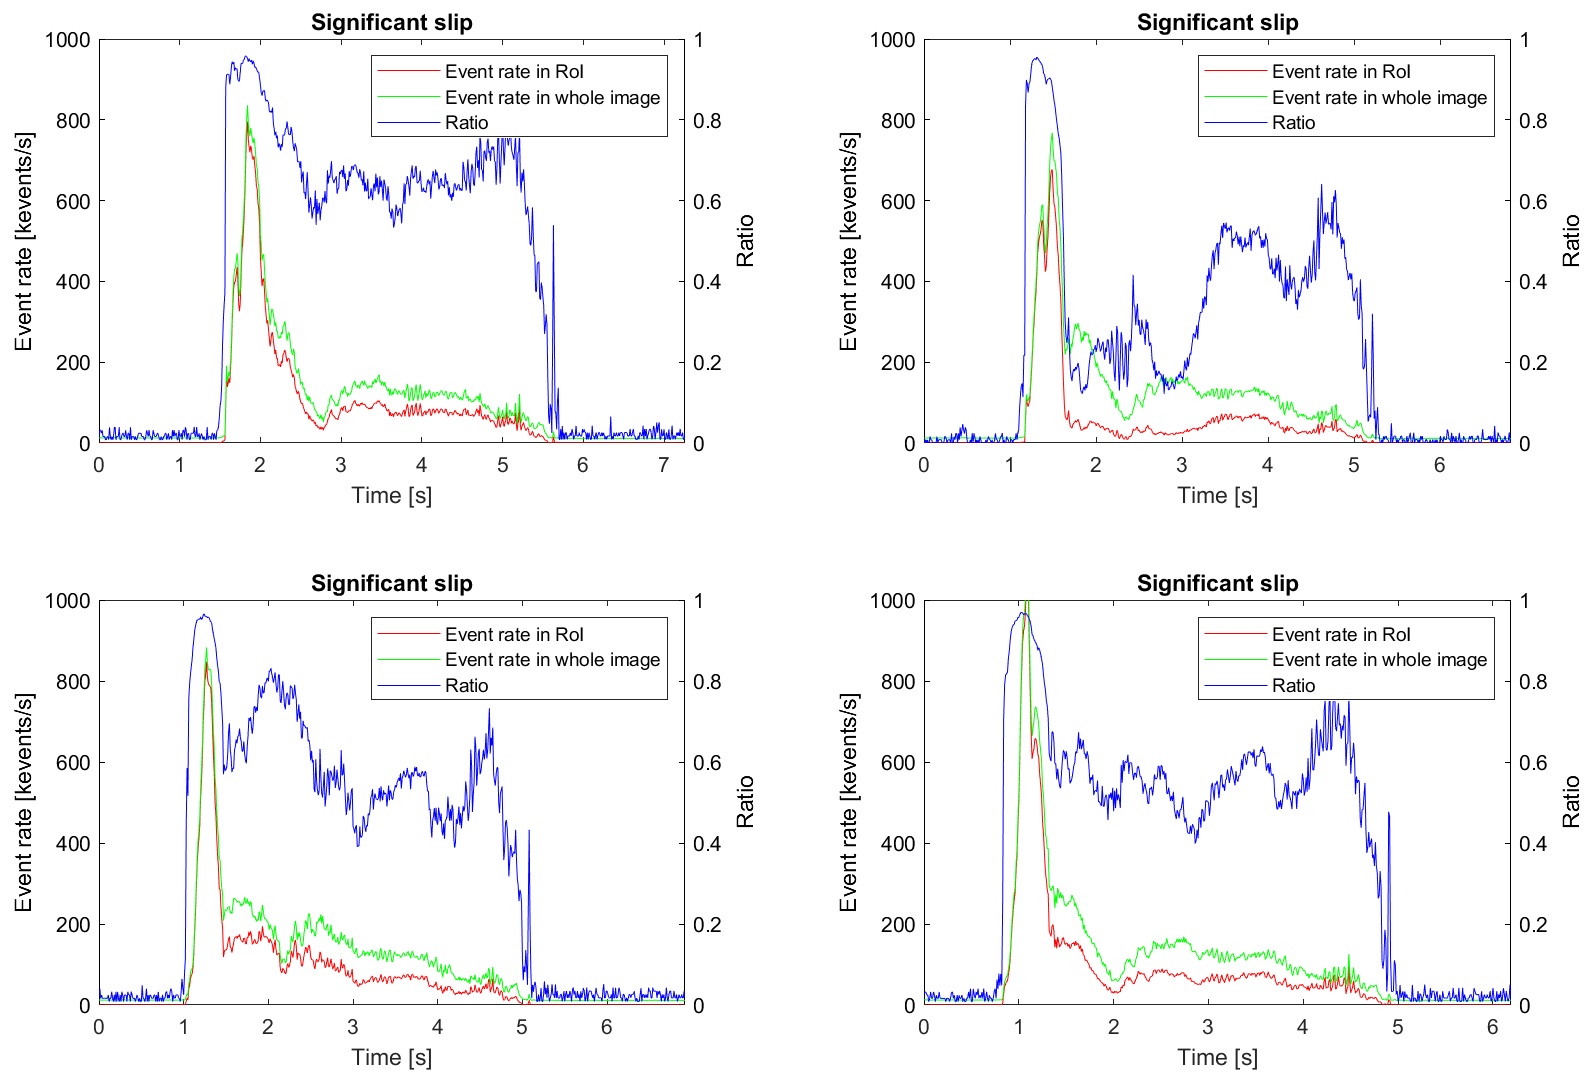
\includegraphics[width=\textwidth]{resources/images/fix_roi_set_rev}
    \caption{Event rate and ratio signals during a pick-and-place motion with a box (reverse grip) using a fixed RoI.}\label{fig:fix_roi_set_rev}
\end{figure}

Using another object, the effect of different texture can be analyzed. For instance, with sequences like the one shown in ~\Cref{fig:set1_case3}, the results reported in ~\Cref{fig:fix_roi_book1} are obtained. As detailed previously, in this sequence there is an initial slip in one direction and then in the opposite direction, which can be detected with the first two peaks of the ratio signal. Moreover, towards the end of the sequence there is a slight movement of the book, which is also detectable in the increasing ratio signal. Finally, the book is placed on the table, but due to its rotation it impacts against it, provoking the last spike in the signal. It is worth noticing how in this case, where the object has much less texture compared to the previous box, meaning that less events are generated by its movement, the ratio threshold suitable for slip detection would be around 0.2, half compared to the previous threshold.

\begin{figure}[h]
    \centering
    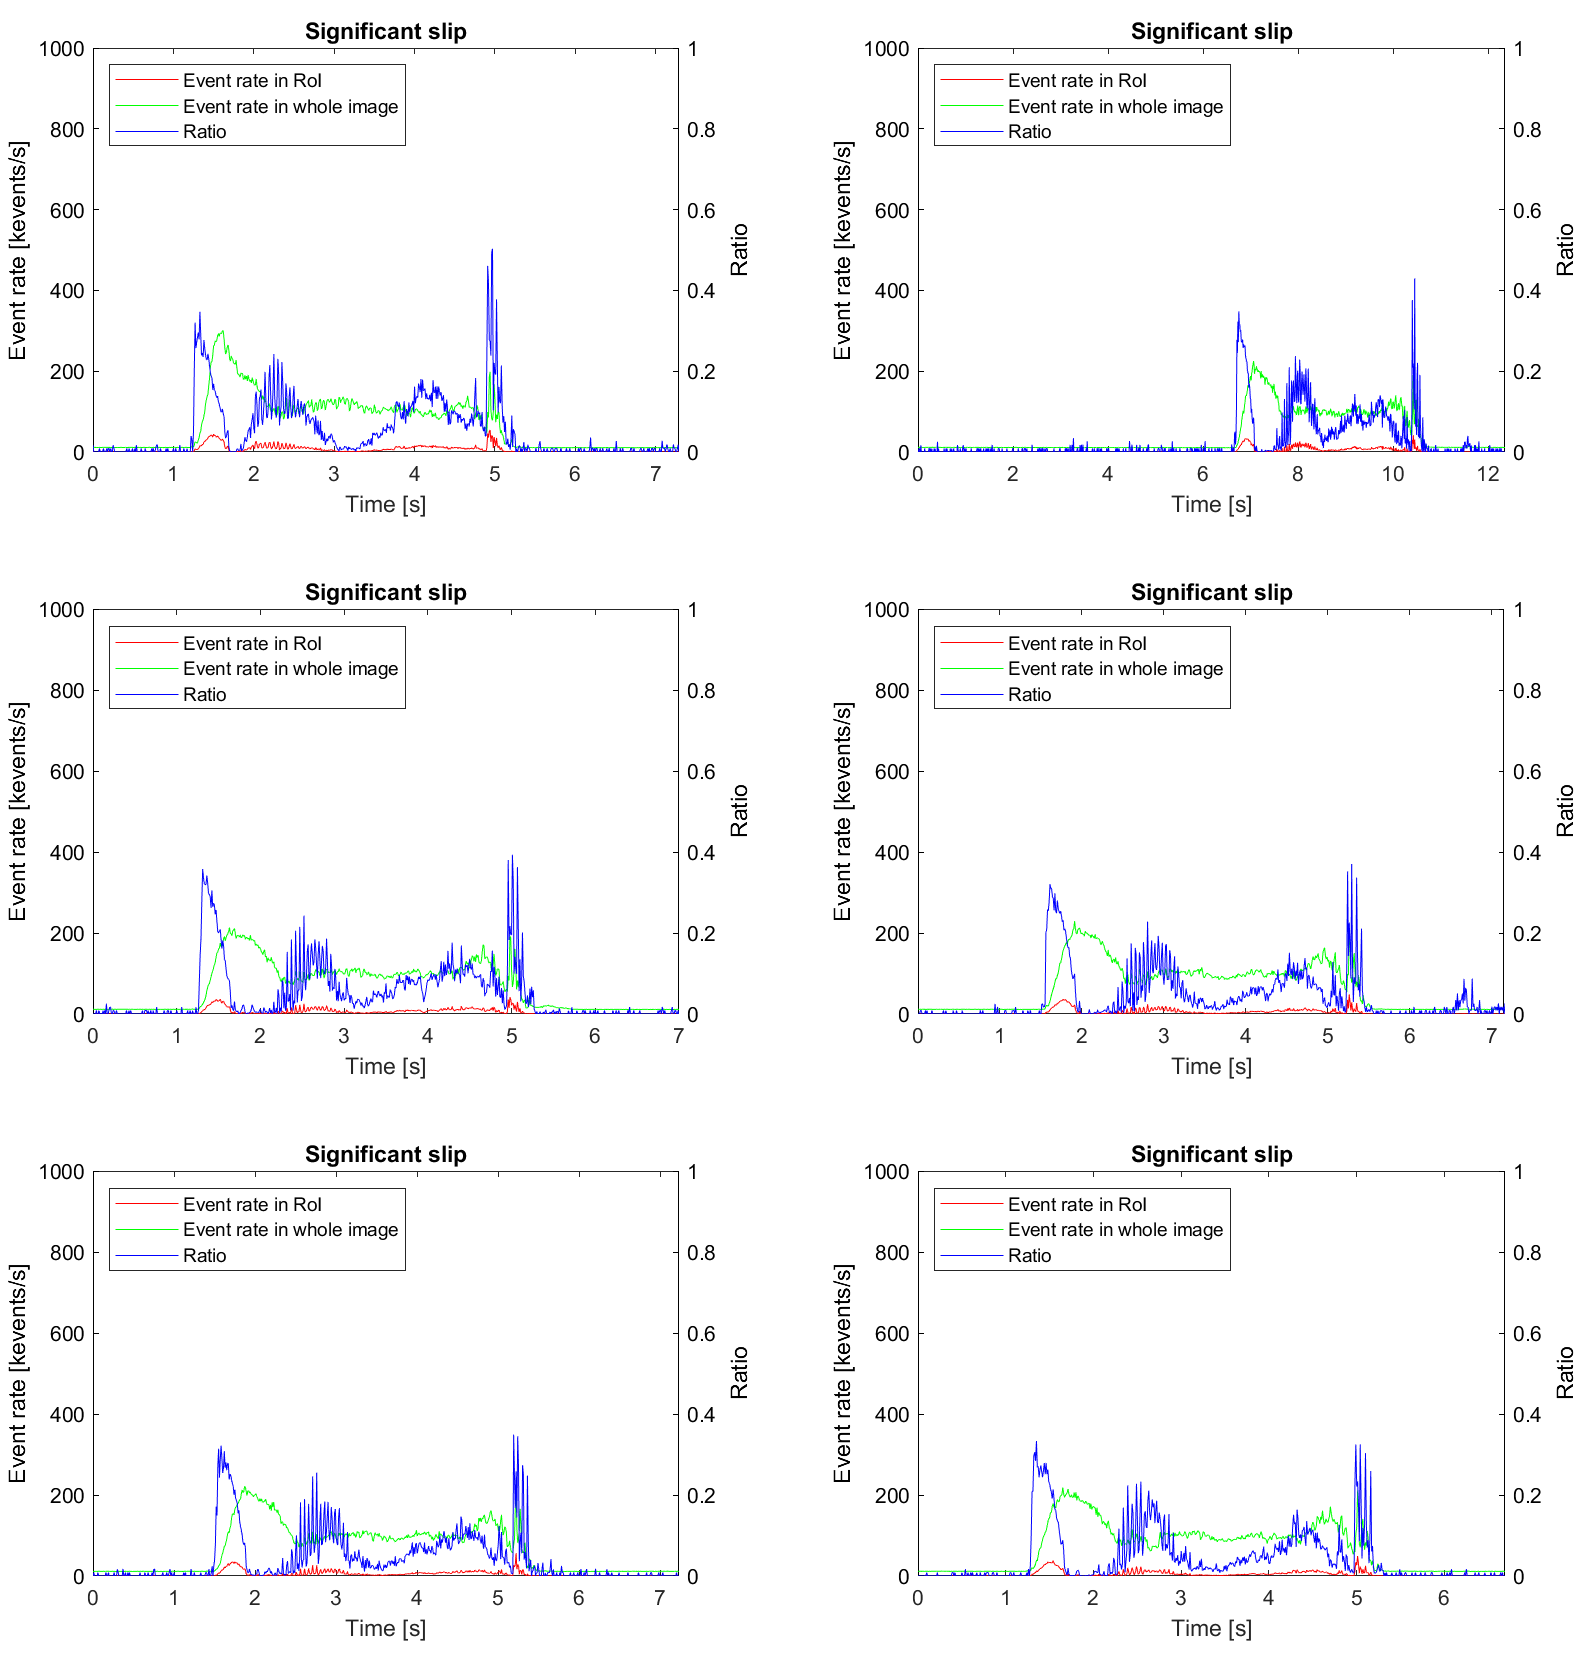
\includegraphics[width=\textwidth]{resources/images/fix_roi_book1}
    \caption{Event rate and ratio signals during a pick-and-place motion with book no. 1 using a fixed RoI.}\label{fig:fix_roi_book1}
\end{figure}

To make it more challenging, the texture of the background can be modified, as happened in the sequence depicted in ~\Cref{fig:set1_case7}, which is the same as ~\Cref{fig:set1_case3}, but adding much more texture to the table. The resulting event rate and ratio signals are reported in ~\Cref{fig:fix_roi_book1_tt}, where similar patterns in the ratio signal are observed, compared to the previous scenario, but now they are not thresholdable for slip detection, due to the high amount of events coming from the background.\\

\begin{figure}[h]
    \centering
    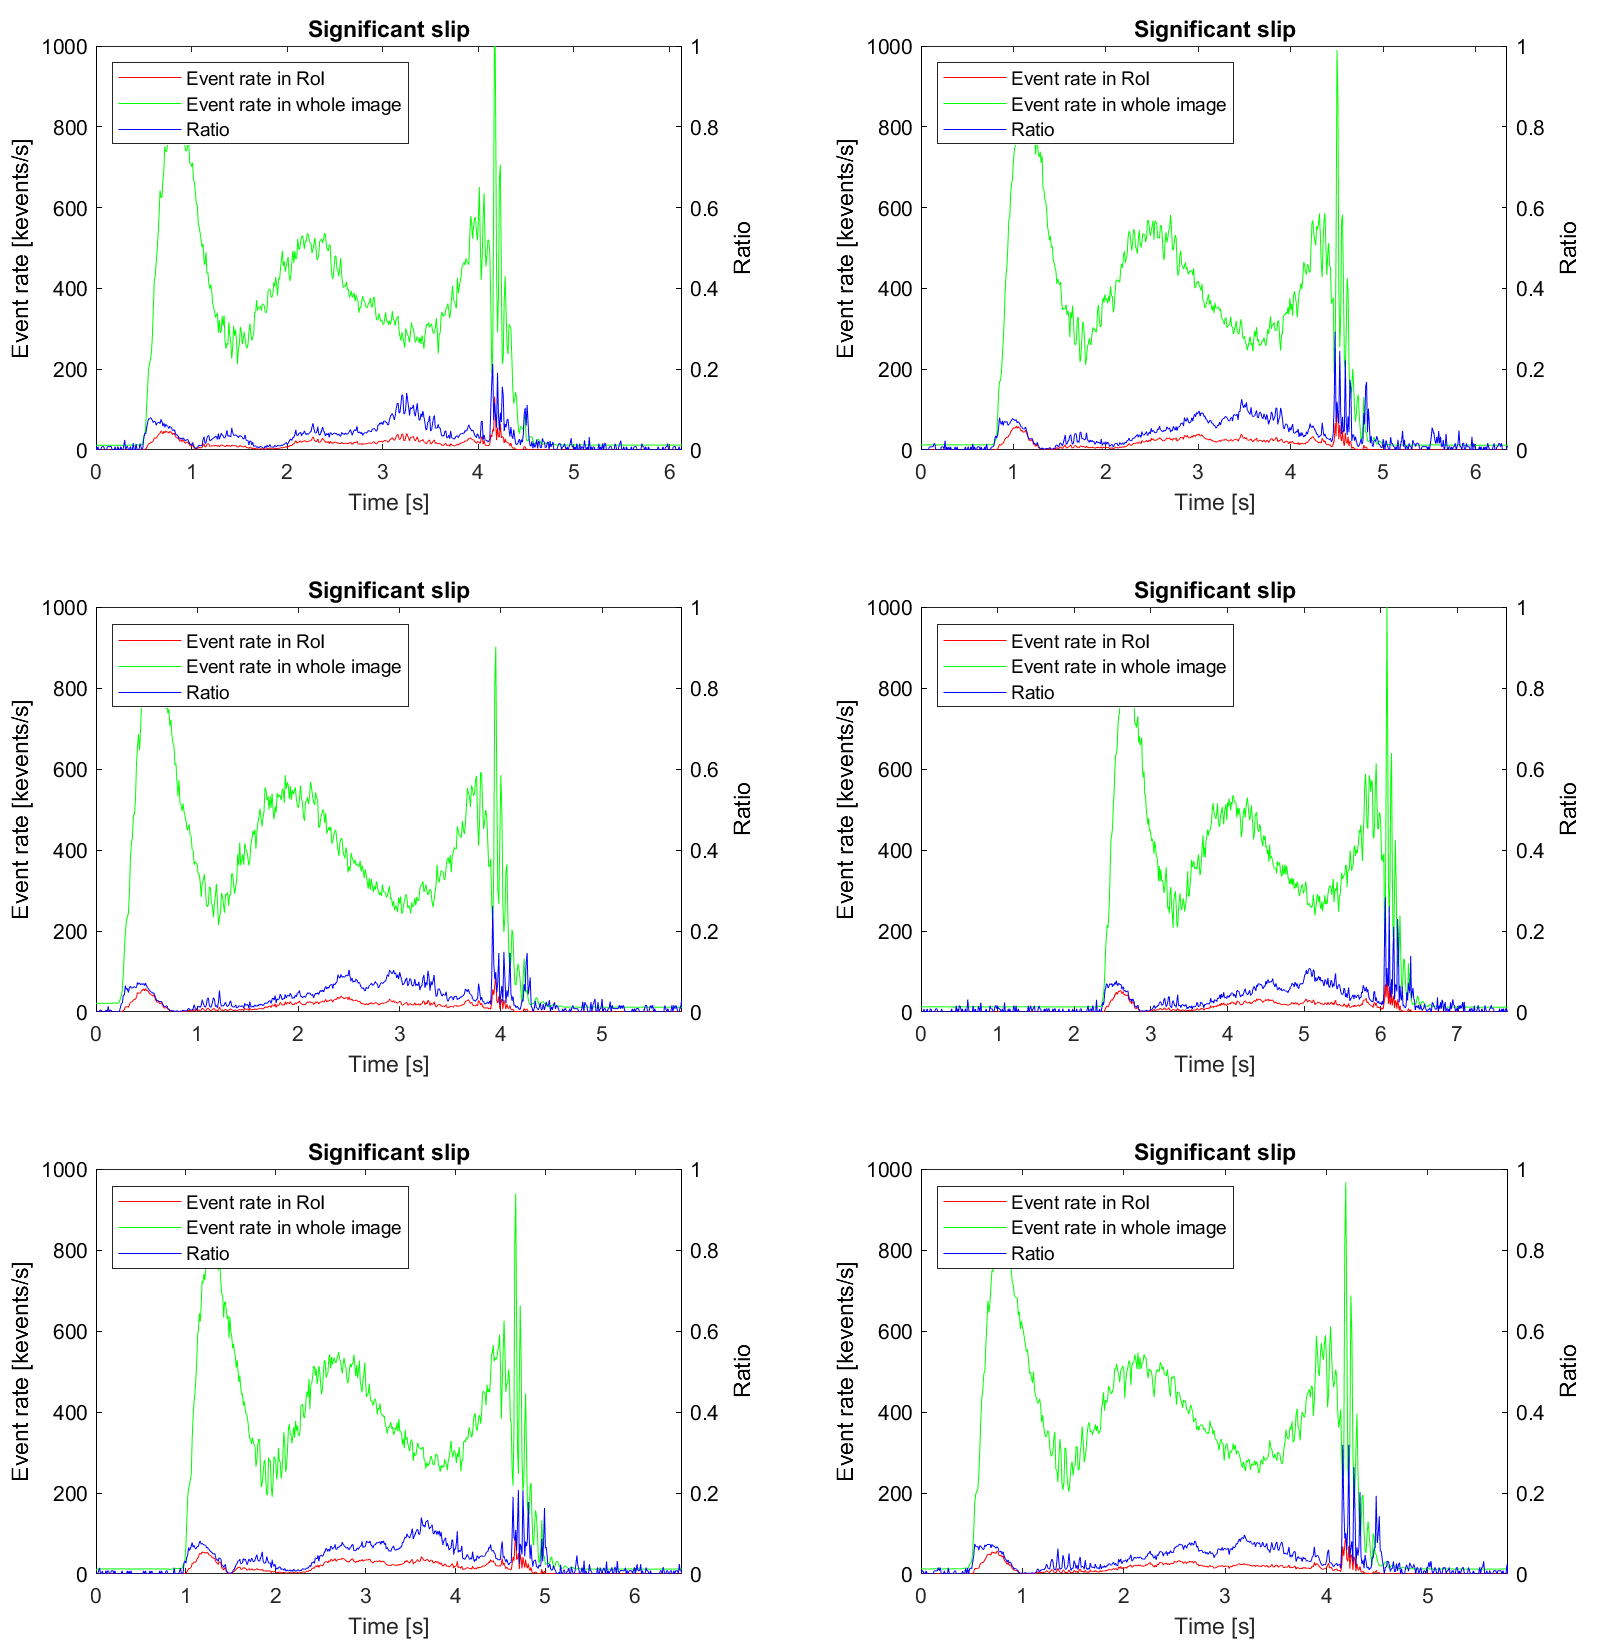
\includegraphics[width=\textwidth]{resources/images/fix_roi_book1_tt}
    \caption{Event rate and ratio signals during a pick-and-place motion with book no. 1 and a highly textured table using a fixed RoI.}\label{fig:fix_roi_book1_tt}
\end{figure}

All in all, this method presents several disadvantages, but shows the potential and limitations of using the ratio signal for slip detection. First, the ratio threshold depends on the texture of the object and also on the background. Additionally, the fixed RoI may not separate the object from the background during the whole sequence, which disables the possibility of slip detection by thresholding the ratio signal.

\subsection{Results with Set 1 and weighted mask}

Using an initially defined fixed RoI, presents the inconvenience of setting it for each scenario and not being valid for cases where the initial and final positions of the object are really different, as for the sequence ~\Cref{fig:set1_case6}. However, as the gripper position in the image plane is known, we have the prior information of where the object is going to be, i.e. between the fingers of the gripper. For each object the width of the gripper is different, but the maximum width is known, which is set as two times the standard deviation, as represented in ~\Cref{fig:gaus_mask}. Then, a gaussian is defined with it along the horizontal direction, with a peak value of 1 in the center of the image and lower values when further from the center. These values are taken into account as weights for the events generated, which depending on the position in which they appear in the image they might have more or less importance. Moreover, the bottom part, which is mostly occupied by the gripper and the camera mount, has a null weight. With this weighted mask, a weighted histogram is computed along time, to generate the event rate and ratio signals.

\begin{figure}[h]
    \centering
    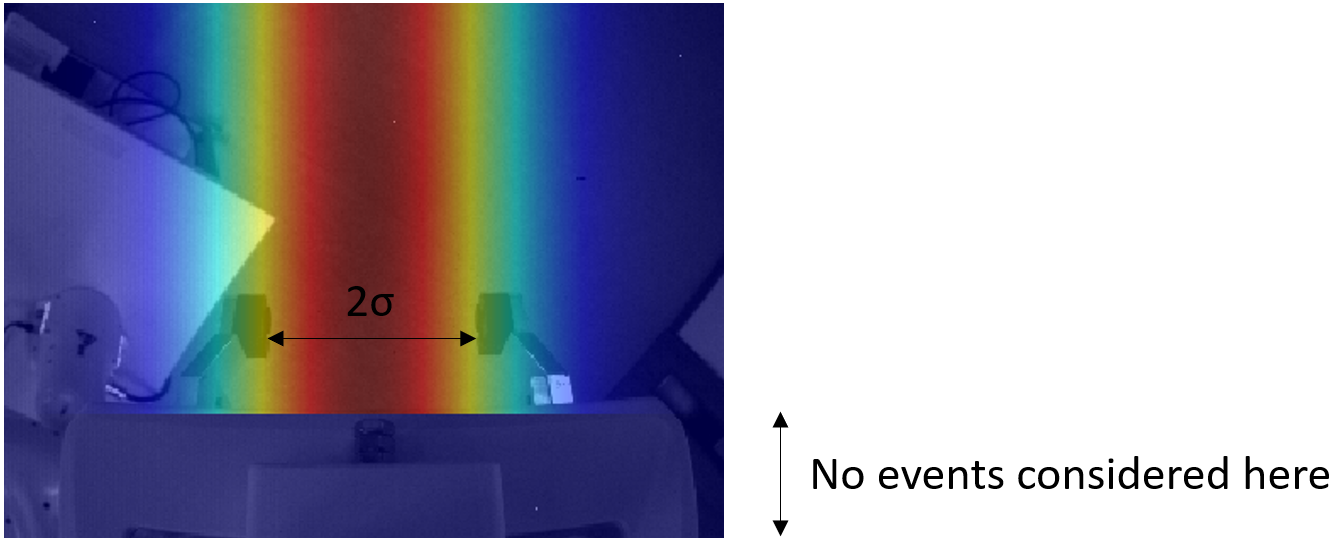
\includegraphics[width=0.8\textwidth]{resources/images/gaus_mask}
    \caption{Description of the weighted (gaussian) mask.}\label{fig:gaus_mask}
\end{figure}

In ~\Cref{fig:fix_mask} some examples of Set 1 with this weighted mask have been depicted.

\begin{figure}[h]
    \centering
    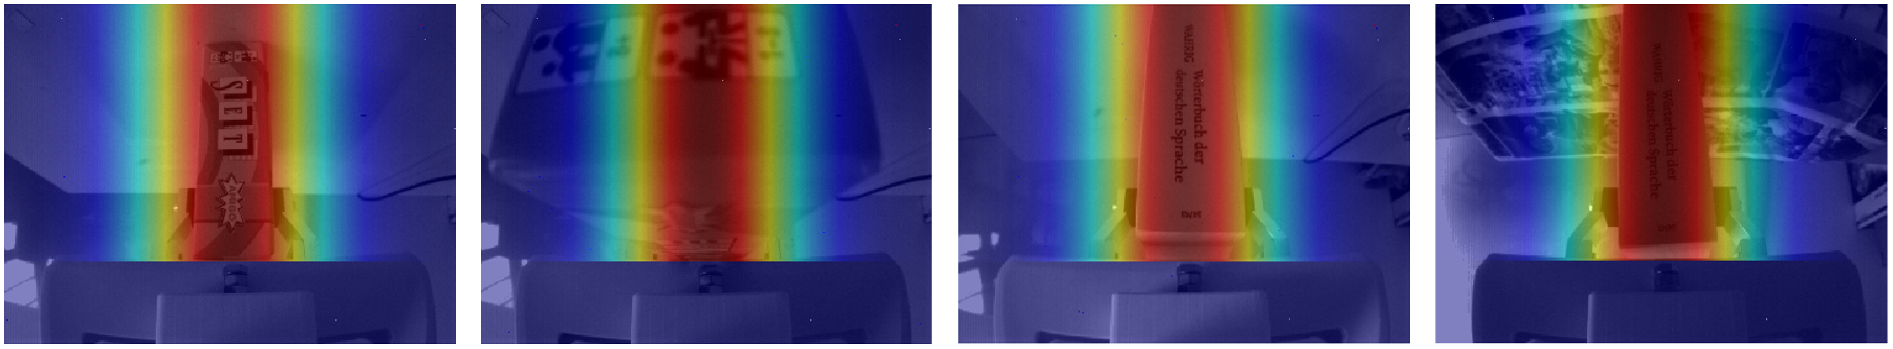
\includegraphics[width=\textwidth]{resources/images/fix_mask}
    \caption{Example initial frames of Set 1, with the weighted mask.}\label{fig:fix_mask}
\end{figure}

A comparison between the fixed RoI and weighted mask approach using some samples of Set 1, is reported in ~\Cref{fig:fix_mask_evr} and ~\Cref{fig:fix_mask_rat}. For the sequence of the box, where almost no slip occurs, we can observe how the weighted event rate is higher than the event rate inside the RoI, as events in the background are also weighted and taken into account. This produces an increase in the ratio values, having higher spikes. When the box slips, both event rates are nearly the same, as the object is mostly in the center of the image. In terms of the ratio, the peaks increase a bit. Overall, the slip detection can still be made, but with a higher threshold, around 0.6.\\

Considering the box with reverse grip, we can see how the weighted event rate is lower after than the RoI one, being significantly different from the event rate in the whole image. This happens as the RoI almost occupied the whole image, as shown in ~\Cref{fig:fix_roi}. Thanks to this adjustment in the event rate, the resulting ratio signal (using the weighted mask) allows us to detect two slips, with a threshold of 0.6 again, which is what happens in the sequence.\\

For book no. 1, in both cases the weighted event rate is higher than the RoI one, but specially in the highly textured table scenario, where many events are generated due to the background, which are weighted in the computation of the event rate. In terms of the ratio signal, the weighted mask shows better results, as using a threshold of 0.2, we can detect the slips, without influencing the highly textured background.

\begin{figure}[H]
    \centering
    \includegraphics[width=\textwidth]{resources/images/fix_mask_evr}
    \caption{Event rate signals during some pick-and-place motions of Set 1 using the fixed RoI and weighted mask.}\label{fig:fix_mask_evr}
\end{figure}

In conclusion, this method solves some of the issues present with the fixed RoI approach:

\begin{itemize}
	\item The weighted mask does not need to be annotated for each scenario, as it is the same for all of them, using the prior of where the object will be grasped.
	\item For the cases where the object rotates a lot and the shape of it varies significantly from the camera's view, it works much better, as the ratio signal can be easily thresholded.
	\item It is more robust to changes in the background's texture.
\end{itemize}

However, the ratio threshold still depends on the object's texture, as for the box we would use 0.6, whereas for the book we would use only 0.2.

\begin{figure}[H]
    \centering
    \includegraphics[width=\textwidth]{resources/images/fix_mask_rat}
    \caption{Ratio signals during some pick-and-place motions of Set 1 using the fixed RoI and weighted mask.}\label{fig:fix_mask_rat}
\end{figure}

\subsection{Results with Set 2 and variable mask}

Another way of dealing with the issues derived from using the fix RoI, is to compute a variable mask where the object is present. For instance, a detection algorithm can be run in the beginning and then the object can be tracked, however, this process can be really computationally expensive, which may be counterproductive when detecting slip using low latency sensors, such as the event-based camera. A naive approach to compute such mask is to record first a sequence without any object and then execute the same pick-and-place operation with different objects. After synchronizing both sequences, the grayscale frames can be subtracted and with that the object can be masked. Concretely, in ~\Cref{fig:var_mask_hb1}, the results of calculating the absolute difference between the sequence in ~\Cref{fig:set2_empty} and ~\Cref{fig:set2_case1} is reported. Then, a binary image is created by thresholding the absolute difference with a value of 50, meaning that any value above or equal than 50 is 1 and the rest 0. After that, some morphological operations are performed in order to get the final mask. Specifically, an opening operation is applied to get rid of the background and then a closing operation is done to fill the gaps in the masked object.

\begin{figure}[H]
    \centering
    \includegraphics[width=\textwidth]{resources/images/var_mask_hb1}
    \caption{Sequence of images with the steps to generate the variable mask. The first column is the subtraction between the empty and with object sequence. The second is generated from the first by computing a binary image. Then, in the third, a opening operation is done and in the fourth a closing one is performed to generate the final mask.}\label{fig:var_mask_hb1}
\end{figure}

At a first, glance we can already realize that this method is quite brittle and present some clear disadvantages:

\begin{itemize}
	\item It is assumed that the background will not change between the initial empty sequence and the rest of experiments. So any change in the initial scene can affect the mask generation.
	\item If there are several objects to be picked (out of the scope of this thesis), all of them will be considered in the mask and not only the one picked.
	\item The object may have similar grayscale value as the background in some occasions and the substraction may not include parts of the object (see  ~\Cref{fig:var_mask_hb1}).
\end{itemize}

It is worth mentioning that the grayscale frames are generated at 40 Hz, therefore, the mask is also updated at this frequency. In ~\Cref{fig:var_mask_hb1_no_slip_evr} and ~\Cref{fig:var_mask_hb1_no_slip_rat}, the results for a non-slip scenario with book no.1 are reported, where we can see that both the event rate and ratio signals are low. Notice that the signals calculated through the weighted fix mask are always higher than the ones from the variable mask, as for the former all the events in the scene are taken into account with the corresponding weight. Note that the signals are only shown during the manipulation phase of the object, where slip should be detected.\\

In contrast, for the slip scenario, the results are shown in ~\Cref{fig:var_mask_hb1_slip_evr} and ~\Cref{fig:var_mask_hb1_slip_rat}. In this case, the ratio signal can be thresholded in both cases to detect the initial peak, corresponding to the main slip, and the second one, which is a slight slip.\\

For book no. 2, in ~\Cref{fig:var_mask_hb2_no_slip_evr} and ~\Cref{fig:var_mask_hb2_no_slip_rat} the results for the non-slip case are reported. By looking at the event rate signals one cannot appreciate any slip, however, the ratio signals present a peak in the beginning which would cause a false positive in terms of slip detection. For the slip case (see ~\Cref{fig:var_mask_hb2_slip_evr} and ~\Cref{fig:var_mask_hb2_slip_rat}), the event rate has an initial and final peak, coinciding with the two slips present in the sequence, but looking at the ratio signal no clear differences can be observed compared to the non-slip case. Hence, this method fails to detect slip in these two sequences.

\begin{figure}[H]
    \centering
    \includegraphics[width=0.86\textwidth]{resources/images/var_mask_hb1_no_slip_evr}
    \caption{Event rate signals of ~\Cref{fig:set2_case1} using the weighted fix and variable mask.}\label{fig:var_mask_hb1_no_slip_evr}
\end{figure}

\begin{figure}[H]
    \centering
    \includegraphics[width=0.86\textwidth]{resources/images/var_mask_hb1_no_slip_rat}
    \caption{Ratio signals of ~\Cref{fig:set2_case1} using the weighted fix and variable mask.}\label{fig:var_mask_hb1_no_slip_rat}
\end{figure}

\begin{figure}[H]
    \centering
    \includegraphics[width=0.86\textwidth]{resources/images/var_mask_hb1_slip_evr}
    \caption{Event rate signals of ~\Cref{fig:set2_case2} using the weighted fix and variable mask.}\label{fig:var_mask_hb1_slip_evr}
\end{figure}

\begin{figure}[H]
    \centering
    \includegraphics[width=0.86\textwidth]{resources/images/var_mask_hb1_slip_rat}
    \caption{Ratio signals of ~\Cref{fig:set2_case2} using the weighted fix and variable mask.}\label{fig:var_mask_hb1_slip_rat}
\end{figure}

\begin{figure}[H]
    \centering
    \includegraphics[width=0.86\textwidth]{resources/images/var_mask_hb2_no_slip_evr}
    \caption{Event rate signals of ~\Cref{fig:set2_case4} using the weighted fix and variable mask.}\label{fig:var_mask_hb2_no_slip_evr}
\end{figure}

\begin{figure}[H]
    \centering
    \includegraphics[width=0.86\textwidth]{resources/images/var_mask_hb2_no_slip_rat}
    \caption{Ratio signals of ~\Cref{fig:set2_case4} using the weighted fix and variable mask.}\label{fig:var_mask_hb2_no_slip_rat}
\end{figure}

\begin{figure}[H]
    \centering
    \includegraphics[width=0.86\textwidth]{resources/images/var_mask_hb2_slip_evr}
    \caption{Event rate signals of ~\Cref{fig:set2_case5} using the weighted fix and variable mask.}\label{fig:var_mask_hb2_slip_evr}
\end{figure}

\begin{figure}[H]
    \centering
    \includegraphics[width=0.86\textwidth]{resources/images/var_mask_hb2_slip_rat}
    \caption{Ratio signals of ~\Cref{fig:set2_case5} using the weighted fix and variable mask.}\label{fig:var_mask_hb2_slip_rat}
\end{figure}

In conclusion, the weighted fix mask and the variable one, present similar results, where the former presents generally higher values in the event rate and ratio signals. Also, the variable mask method requires of extra computations to get this changing mask, which comes with the cost of being highly dependent on the background and the changes that may occur between the initial empty sequence compared to the following pick-and-place motions.

\section{Optical flow analysis}

\subsection{Introduction}

By looking at the moving edges in the event images, the motion of the object can be distinguished. Also, the event rate gives a notion of how the velocity of the object increases. However, for this purpose, per pixel velocity in each axis of the image may be more suitable. Actually, the motion estimation can be done through optical flow, which is the pattern of apparent motion of objects, surfaces and edges in a visual scene caused by the relative motion between an observer and a scene.\\

Concretely, we use EV-FlowNet ~\cite{evflownet}, a self-supervised deep learning pipeline for optical flow estimation for event-based cameras. 

\subsection{Results with Gelsight dataset}

First, optical flow was analyzed with the Gelsight dataset ~\cite{gelsight2018}. The EV-FlowNet algorithm outputs the pixel-wise velocities in \textit{x} and \textit{y} axis of the image, given the grayscale frames and the events. These velocities are given at 40 Hz, which corresponds to the rate at which the grayscale images are provided.\\

At each instant, the absolute mean velocity in each direction is computed (for all the pixels in the image). In addition, the pixels where the velocity norm is nearly zero (considered as any value lower than 0.01) are removed from the mean, in order to have a variation in the mean when there is motion coming from the object. In ~\Cref{fig:gelsight_of}, the absolute mean velocities in \textit{x} and \textit{y} directions for 4 samples of object 1 have been reported. Due to the EV-FlowNet algorithm, the estimation is only provided until 0.6 s, instead of reaching the total duration (1 s) of the sequence.\\

During a perfect grasp, as happens in the sequence ~\Cref{fig:gelsight_case1}, with a gripper width of 66.6 mm, the velocities are nearly zero during the whole sequence.\\

For the sequences represented in ~\Cref{fig:gelsight_case2} and ~\Cref{fig:gelsight_case3}, with a gripper width of 67.2 and 67.3 mm respectively, there is a slight slip in the beginning that stops. This behavior can also be analyzed by looking at the velocities, having a small peak in the velocities for a width of 67.2 mm and a higher peak for 67.3 mm. However, the later width produces a failure in the grasping just in the end, which cannot be detected by looking at the velocities, as the data is cropped to 0.6 s.\\

Finally, in a scenario where the gripper fails to grasp the object, as happened in ~\Cref{fig:gelsight_case4}, with a gripper width fo 67.5 mm, the velocities are high during the whole sequence, as the object stays in the table while the gripper and the attached camera move away from it.

\begin{figure}[h]
    \centering
    \includegraphics[width=\textwidth]{resources/images/gelsight_of}
    \caption{Comparison of the absolute mean velocities evolution in the whole image for 4 samples of object 1 from the dataset in ~\cite{gelsight2018}.}\label{fig:gelsight_of}
\end{figure}

\subsection{Results with Set 1}

The output from optical flow can be coded into HSV (Hue Saturation and Value) format for visualizing the data. Concretely, the hue encodes the angle of the velocity, the saturation represents the norm of it and the value is set at its maximum always. In ~\Cref{fig:OF_angle} the encoding of the norm and angle are depicted, where the angles show different colors and the norm regulates their intensity.\\

\begin{figure}[h]
    \centering
    \includegraphics[width=0.8\textwidth]{resources/images/OF_angle}
    \caption{Colomap resulting from the encoding of the norm and angle of the optical flow velocities.}\label{fig:OF_angle}
\end{figure}

In ~\Cref{fig:OF_set_no_slip}, the motion estimation for a non-slip case is shown. As one may notice, there is no motion in the center of the image, precisely where the object is. Instead, in ~\Cref{fig:OF_set_slip}, in the first two rows the motion of the object can be clearly seen, coinciding with the slips. First, a rotation occurs in one direction, such that the object moves downwards in the image plane. The estimated motion shown for this case is represented by the colors pink, purple and dark blue, which precisely correspond to the observed vertical motion downwards, as indicated in ~\Cref{fig:OF_angle}. On the contrary, the second rotation happens inn the opposite direction, such that the object moves upwards in the image plane. The estimated motion shown for this case is represented by the colors green and yellow, which precisely correspond to the observed vertical motion upwards, as indicated in ~\Cref{fig:OF_angle}.

\begin{figure}[H]
    \centering
    \includegraphics[width=\textwidth]{resources/images/OF_set_no_slip}
    \caption{Event images (first column), motion flow estimation using optical flow (second column) and grayscale frames (third column) for the sequence in ~\Cref{fig:set1_case1}.}\label{fig:OF_set_no_slip}
\end{figure}

\begin{figure}[H]
    \centering
    \includegraphics[width=\textwidth]{resources/images/OF_set_slip}
    \caption{Event images (first column), motion flow estimation using optical flow (second column) and grayscale frames (third column) for the sequence in ~\Cref{fig:set1_case2}.}\label{fig:OF_set_slip}
\end{figure}

Moreover, for the reverse grip, where the motion is quite abrupt, the resulting motion estimation for a concrete instant is depicted in ~\Cref{fig:OF_set_rev}. Here, there is a predominant vertical motion upwards, indicated by the green and yellow colors. However, in the left and right edges of the object, the pixels are moving towards the center, producing a horizontal motion in them, which is depicted with the red and cyan colors.

\begin{figure}[H]
    \centering
    \includegraphics[width=\textwidth]{resources/images/OF_set_rev}
    \caption{Event images (first column), motion flow estimation using optical flow (second column) and grayscale frames (third column) for the sequence in ~\Cref{fig:set1_case6}.}\label{fig:OF_set_rev}
\end{figure}

Using book no. 1, as depicted in ~\Cref{fig:OF_hb1}, we can also detect vertical motion with green and purple colors. However, if the same experiment is repeated with a highly textured background, as reported in ~\Cref{fig:OF_hb1_tt}, the motion estimated for the background is predominant and the one for the object during slip is interpolated from the background, regarding the angle of the velocities.

\begin{figure}[H]
    \centering
    \includegraphics[width=\textwidth]{resources/images/OF_hb1}
    \caption{Event images (first column), motion flow estimation using optical flow (second column) and grayscale frames (third column) for the sequence in ~\Cref{fig:set1_case3}.}\label{fig:OF_hb1}
\end{figure}

\begin{figure}[H]
    \centering
    \includegraphics[width=\textwidth]{resources/images/OF_hb1_tt}
    \caption{Event images (first column), motion flow estimation using optical flow (second column) and grayscale frames (third column) for the sequence in ~\Cref{fig:set1_case7}.}\label{fig:OF_hb1_tt}
\end{figure}

These motion flow plots are informative visually, but not directly useful for slip detection. To this end, the absolute mean velocity for each axis is computed, as previously described. The differences with the Gelsight dataset are that now the object and the background motion should be somehow separated and we are interested in the vertical motion, as all examples suffer from the described rotational slip. To focus on the motion produced by the object, we can use the fixed RoI approach or the weighted mask one, which were used for generating the event rate and ratio signals.\\

First, for a non-slip case, as reported in ~\Cref{fig:OF_comparison_set_no_slip}, there is a nearly zero velocity in the vertical axis (\textit{y}), which would indicate that there is no vertical motion in the object, meaning no slip occurred. For the horizontal axis (\textit{x}), we can see a peak in the beginning, due to the background, which is not perfectly separated from the object in both cases. In contrast, in a slip example, shown in ~\Cref{fig:OF_comparison_set}, there are two evident peaks in the vertical velocity, which correspond to the two rotational slips present in the sequence. Concretely, for the weighted mask approach the signal presents higher values. Moreover, in the reverse grip example (see ~\Cref{fig:OF_comparison_set_rev}), the vertical motion again shows how there is a slip in the beginning of the experiment. As previously pointed out, in this example, there is also horizontal motion in some parts of the object, which produces as well a peak in the velocity in \textit{x}.\\

For the book experiment, as observed in ~\Cref{fig:OF_comparison_hb1}, the fixed RoI approach presents two small peaks, one in the beginning and one in the end, due to the two small slips present in the experiment. However, for the weighted mask approach, there are several spikes in the middle of the sequence, producing false positives, which may be due to the background's motion. 

\begin{figure}[H]
    \centering
    \includegraphics[width=0.95\textwidth]{resources/images/OF_comparison_set_no_slip}
    \caption{Comparison of the absolute mean velocities evolution in the whole image for the sequence in ~\Cref{fig:set1_case1}.}\label{fig:OF_comparison_set_no_slip}
\end{figure}

\begin{figure}[H]
    \centering
    \includegraphics[width=0.95\textwidth]{resources/images/OF_comparison_set}
    \caption{Comparison of the absolute mean velocities evolution in the whole image for the sequence in ~\Cref{fig:set1_case2}.}\label{fig:OF_comparison_set}
\end{figure}

\begin{figure}[H]
    \centering
    \includegraphics[width=0.95\textwidth]{resources/images/OF_comparison_set_rev}
    \caption{Comparison of the absolute mean velocities evolution in the whole image for the sequence in ~\Cref{fig:set1_case6}.}\label{fig:OF_comparison_set_rev}
\end{figure}

\begin{figure}[H]
    \centering
    \includegraphics[width=0.95\textwidth]{resources/images/OF_comparison_hb1}
    \caption{Comparison of the absolute mean velocities evolution in the whole image for the sequence in ~\Cref{fig:set1_case3}.}\label{fig:OF_comparison_hb1}
\end{figure}

Finally, if a highly textured background is present, we saw that the angle of the velocities in the object are not properly estimated, being interpolated from the background. This behavior can also been observed in the velocity signals, depicted in ~\Cref{fig:OF_comparison_hb1_tt}, where the initial peak, corresponding to the slip, is more present in the horizontal axis than the vertical one, while the slip produces vertical motion.

\begin{figure}[H]
    \centering
    \includegraphics[width=0.95\textwidth]{resources/images/OF_comparison_hb1_tt}
    \caption{Comparison of the absolute mean velocities evolution in the whole image for the sequence in ~\Cref{fig:set1_case7}.}\label{fig:OF_comparison_hb1_tt}
\end{figure}

\section{Conclusion}

In this chapter two slip detection methods have been analyzed in detail. First, the event rate and ratio signals have been discussed, using different ways of separating the object from the background. The results have shown how the weighted mask and variable mask approaches are more informative and robust to detect rotational slip, compared to the fixed RoI method, which fails in highly textured backgrounds and  sequences where the object's shape changes significantly from the camera's view. Both of them present similar results, but the weighted mask approach is much more simpler and does not depend on the pre-recorded empty handed pick-and-place sequence, which may differ from the subsequent experiments, making it quite brittle.\\

Moreover, the optical flow results have been transformed into two 1D signals, the horizontal and vertical absolute mean velocities. These velocities have been computed for the fixed RoI and weighted mask approaches and the results show that the rotational slip coincides, ideally, with high-speed vertical motion in the object. Therefore, it would be enough to threshold the vertical absolute mean velocity signal, in order to detect slip. However, in highly textured backgrounds, the orientation of the motion is not properly estimated, producing the peaks also in the horizontal absolute mean velocity signal. In terms of the methods used to separate the object's motion from the background, the fixed RoI works robustly in all scenarios, while the weighted mask approach fails in one of the experiments, producing false positives.\\

There is no doubt that both presented methods, event rate and optical flow, are informative about rotational slip. However, the designed 1D signals, which were intended to be thresholded and detect slip if the value was above this threshold, are not robust enough to work in different scenarios. In the case of the ratio signal, it is easier to threshold as it is bounded between 0 and 1. On the contrary, the vertical absolute mean velocity signal is not bounded, thus it is more complicated set a limit.\\

All in all, these handcrafted 1D signals are a first step to understand slip detection, but are not enough to generalize in different scenarios and detect slip robustly.







    \cleardoublepage
\chapter{Conclusions}\label{sec:conclusions}

\section{Summary}

In this work, we perform an exploration of different methods for slip detection during object manipulation in pick-and-place operations using a robot arm with an attached event-based camera, which presents several advantages over frame-based cameras, making it really appropriate for highly responsive systems. Concretely, it has high temporal resolution, low latency, high dynamic range and low power consumption.\\

First, we designed and built the experimental setup, which consists of a robot system, called Panda, including a robot arm and its controller, a two-finger parallel gripper to manipulate the object, the DAVIS 346 camera and a computer connected to it and to the controller of the robot arm and gripper. In addition, to attach the DAVIS 346 to the robot arm and gripper, a mount has been designed and printed, in order to have an external view of the contact between the object and the gripper, while having the camera robustly attached to the robot and offering flexibility when it comes to the position and orientation of the camera with respect to the gripper. Moreover, the software has been set up to execute a desired trajectory during the pick-and-place motion.\\

Then, some small sets of data were recorded, containing slip and non-slip cases during pick-and-place motions with different objects and backgrounds. After analyzing different ways of inducing slip and grasping failures, we focused our efforts in off-centered grasping to produce rotational slip. In total three sets of data have been collected, which have been studied and analyzed iteratively to discover new sources of information that were necessary to be recorded, generating the necessity of recording new sets of data.\\

In terms of the methods tested to determine slip cases, they can be classified in two main groups, depending on the source of information used. On the one hand, the first one considers that whenever a slip occurs, the object moves with respect to the camera (also to the robot arm and gripper), which generates events due to the texture of the object, producing an increase in the number of events in the region where the object is present. To separate the object from the background, three ways have been analyzed and compared, namely, the fixed RoI, the weighted mask and the variable mask approaches. Once the events from the object are separated, the event rate and ratio signals are computed, which can be thresholded to detect slip. On the other hand, a slip can be detected by estimating the motion of the scene through optical flow, which is obtained using EV-FlowNet ~\cite{evflownet}. Whenever, a rotational slip occurs, the object presents mainly vertical motion, that is why the horizontal and vertical absolute mean velocities are computed separately, so that thresholding the vertical one, slip can be detected. To separate the object's motion from the background, in this case, the fixed RoI and weighted mask approaches have been compared.\\

For the ratio signal, the fixed RoI presents several disadvantages, e.g. it needs to be annotated for each experiment, it fails in cases where the object's shape changes significantly from the camera's view and it is not robust to changes in the background's texture. With the weighted mask approach these issues are solved, however the threshold still depends on the object's texture. Moreover, the weighted mask and variable mask approaches present similar results, but the variable mask one is quite brittle and requires of extra computations.\\

On the contrary, for the vertical absolute mean velocity signal, the fixed RoI works robustly in all scenarios, while the weighted mask approach fails in one of the experiments, producing false positives.\\

Both described methods are informative about rotational slip, however, the ratio signal is easier to threshold, as it is bounded between 0 and 1, compared to the vertical absolute mean velocity one, which is not bounded.

\section{Limitations and Future Work}

The designed 1D signals, which were intended to be thresholded and detect slip, are not robust enough to work in different scenarios. The ratio signal is sometimes not enough to differentiate between a non-slip and a slip case and in highly textured backgrounds, the orientation of the motion is not properly estimated, thus, the vertical absolute mean velocity may not be enough to detect slip. All in all, these handcrafted 1D signals are a first step to understand slip detection, but are not enough to generalize in different scenarios and detect slip robustly.\\

There are several ideas that we had in mind, but could not execute them in the time frame of this thesis. First, in Set 2, the camera's angular velocity was recorded along with the other data to compute the motion flow of the scene. The idea behind that is to estimate the background's motion through these known velocities and compare them to the optical flow, in order to detect anomalies between the predicted motion and the real one, being these anomalies, independent motion corresponding to slips.\\

Also, in order to separate the object properly from the background, we tried to identify independently moving objects in the scene, where the background should be identified ideally as a single object and the manipulated object, if there is no slip, it is not a moving object, but if it rotates it should be identified as another independently moving object. We tried to use a novel event-based motion segmentation method ~\cite{motionsegmentation}, but the segmentation was not properly done. Therefore, we assume that the algorithm needs to be fine-tuned to our concrete problem, constraining to the kind of motion we are executing. However, this implies the modification of the motion segmentation code, which is out of the scope of this work.\\

We have seen that the ratio of events and the vertical velocity are informative of slip detection, however, thresholding these signals is not generalizable. Therefore, this information can be used as input to supervised learning methods. Nevertheless, to explore this possibility and be able to train and validate the models, much more data is needed, which includes repeated pick-and-place motions of diverse daily use objects with balanced non-slip and slip cases. Moreover, this dataset should be labeled, which can be done using the motion capture system, i.e. the OptiTrack. To this end, Set 3 was recorded, where the relative pose between the gripper and the object changes when there is a slip. This motion capture system can be used as ground-truth, but not for usual slip detection, as the system is not practical nor flexible to use in general scenarios.\\

Finally, the slip detection problem can be analyzed in non-cluttered environment, picking one object among several objects, which is a more realistic scenario but considered out of the scope of this thesis.\\

Once this rotational slip detection problem is solved, linear slip and other grasping failures should be considered. Moreover, to complete the ARA project, once these slips and grasp failures are detected, the pick-and-place motion should be modified appropriately in order to complete it successfully, using the feedback of the slip and failure detection algorithm.



    \nolinenumbers
    \cleardoublepage

    \cleardoublepage
    \cleardoublepage
\chapter*{Bibliography}
\mtcaddchapter\addstarredchapter{Bibliography}
\markboth{Bibliography}{Bibliography}
\stepcounter{chapter}
\renewcommand*{\chapterthumbformat}{Bibliography}

\printbibliography[heading=empty,category=cited,sorting=none]



    \backmatter
\end{document}
% ------------------------------------------------------------------------------
